% interacttfssample.tex
% v1.05 - August 2017
\documentclass[]{interact}
\usepackage[utf8]{inputenc}
\usepackage{times}
\usepackage{microtype}
\usepackage{lscape}

\usepackage{epstopdf}% To incorporate .eps illustrations using PDFLaTeX, etc.

%\usepackage[caption=false]{subfig}% Support for small, `sub' figures and tables

%\usepackage[nolists,tablesfirst]{endfloat}% To `separate' figures and tables from text if required

%\usepackage[doublespacing]{setspace}% To produce a `double spaced' document if required
%\setlength\parindent{24pt}% To increase paragraph indentation when line spacing is doubled
%\setlength\bibindent{2em}% To increase hanging indent in bibliography when line spacing is doubled

\usepackage[numbers,sort&compress]{natbib}% Citation support using natbib.sty  %

\usepackage{subfigure}
\usepackage{multirow,slashbox}
\usepackage{array}
\usepackage{float}
\usepackage{soul}
\usepackage{xcolor}
\graphicspath{{./images/}}


\bibpunct[, ]{[}{]}{,}{}{,}{,}% Citation support using natbib.sty
\renewcommand\bibfont{\fontsize{10}{12}\selectfont}% Bibliography support using natbib.sty

\theoremstyle{plain}% Theorem-like structures provided by amsthm.sty
\newtheorem{theorem}{Theorem}[section]
\newtheorem{lemma}[theorem]{Lemma}
\newtheorem{corollary}[theorem]{Corollary}
\newtheorem{proposition}[theorem]{Proposition}

\theoremstyle{definition}
\newtheorem{definition}[theorem]{Definition}
\newtheorem{example}[theorem]{Example}

\theoremstyle{remark}
\newtheorem{remark}{Remark}
\newtheorem{notation}{Notation}

\newenvironment{changemargin}[2]{%
\begin{list}{}{%
\setlength{\topsep}{0pt}%
\setlength{\leftmargin}{#1}%
\setlength{\rightmargin}{#2}%
\setlength{\listparindent}{\parindent}%
\setlength{\itemindent}{\parindent}%
\setlength{\parsep}{\parskip}%
}%
\item[]}{\end{list}} 

%% Add a new subsection
\usepackage{titlesec}
\usepackage{hyperref}

\titleclass{\subsubsubsection}{straight}[\subsection]

\newcounter{subsubsubsection}[subsubsection]
\renewcommand\thesubsubsubsection{\thesubsubsection.\arabic{subsubsubsection}}
\renewcommand\theparagraph{\thesubsubsubsection.\arabic{paragraph}} % optional; useful if paragraphs are to be numbered

\titleformat{\subsubsubsection}
  {\normalfont\normalsize\bfseries}{\thesubsubsubsection}{1em}{}
\titlespacing*{\subsubsubsection}
{0pt}{3.25ex plus 1ex minus .2ex}{1.5ex plus .2ex}

\makeatletter
\renewcommand\paragraph{\@startsection{paragraph}{5}{\z@}%
  {3.25ex \@plus1ex \@minus.2ex}%
  {-1em}%
  {\normalfont\normalsize\bfseries}}
\renewcommand\subparagraph{\@startsection{subparagraph}{6}{\parindent}%
  {3.25ex \@plus1ex \@minus .2ex}%
  {-1em}%
  {\normalfont\normalsize\bfseries}}
\def\toclevel@subsubsubsection{4}
\def\toclevel@paragraph{5}
\def\toclevel@paragraph{6}
\def\l@subsubsubsection{\@dottedtocline{4}{7em}{4em}}
\def\l@paragraph{\@dottedtocline{5}{10em}{5em}}
\def\l@subparagraph{\@dottedtocline{6}{14em}{6em}}
\makeatother

\setcounter{secnumdepth}{4}
\setcounter{tocdepth}{4}
%%

\begin{document}

%\articletype{ARTICLE TEMPLATE}% Specify the article type or omit as appropriate

\title{Hilbert space methods to approximate Gaussian processes using Stan}

%\author{
%\name{}
%\affil{\textsuperscript{a}Department of Cartographic Engineering, Geodesy, and Photogrammetry, Universitat Polit\`ecnica de Val\`encia, Spain; }
%}

\maketitle

\begin{abstract}

\end{abstract}

\begin{keywords}
Gaussian processes; Low-rank Gaussian processes; Hilbert Space methods; Sparse Gaussian processes
\end{keywords}

\tableofcontents


%Contents
\newpage

\section{Introduction}\label{sec_bf_intro}

Gaussian processes (GPs) are flexible statistical models for specifying probability distributions over multi-dimensional non-linear functions \citep{rasmussen2006gaussian,neal1997monte}. Their name stems from the fact that any finite set of function values is jointly distributed as a multivariate Gaussian. GPs are defined by a mean and a covariance function. The covariance function encodes our prior assumptions about the functional relationship, such as continuity, smoothness, periodicity and scale properties. GPs not only allow for non-linear effects but can also implicitly handle interactions between covariates. Different types of covariance functions can be combined for further increased flexibility. Due to their generality and flexibility, GPs are of broad interest across machine learning and statistics \citep{rasmussen2006gaussian,neal1997monte}. Among others, they find application in the fields of spatial epidemiology \citep{diggle2013statistical,carlin2014hierarchical}, robotics and control \citep{deisenroth2015gaussian}, signal processing \citep{sarkka2013spatiotemporal}, as well as Bayesian optimization and probabilistic numerics \citep{roberts2010bayesian,briol2015probabilistic,hennig2015probabilistic}.

Given $n$ observations in the data, the computational complexity and memory requirements of exact GP implementation in general scale as $O(n^3)$ and $O(n^2)$, respectively. This limit their application to rather small data sets of a few tens of thousands observations at most. The problem becomes more severe when performing full Bayesian inference via sampling methods, where in each sampling step we need $O(n^3)$ computations when inverting the Gram matrix of the covariance function, usually through Cholesky factorization. To alleviate these computational demands, several approximate methods have been proposed. 

Sparse GPs are based on low-rank approximations of the covariance matrix. The low-rank approximation with $m \ll n$ {\it inducing points} implies reduced memory requirements of $O(nm)$ and corresponding computational complexity of $O(nm^2)$.
A unifying view on sparse GPs based on approximate generative methods
is provided in \cite{quinonero2005unifying}, while a general review
can be found in \cite{rasmussen2006gaussian}. \citet{Burt+Rasmussen+vanderWilk:2019} show that for regression with normally distributed covariates in $D$ dimensions and using the squared exponential covariance function, $M=O(\log^DN)$ is sufficient for accurate approximation.
% More recent developments in the context of sparse GPs include a structured kernel interpolation method \citep{wilson2015kernel}. More recently, \citep{bui2017unifying} proposed to use inducing points-based sparse approximation methods to perform GP approximations at inference time rather than at modeling time.

An alternative class of low-rank approximations is based on forming a basis function approximation with $m \ll n$ basis functions. The basis functions are usually presented explicitly, but can also be used to form a low rank covariance matrix approximation. Common basis function approximations rest on the spectral analysis and series expansions of Gaussian processes \citep{loeve1977probability,trees1968detection,adler1981geometry,cramer2013stationary}.
Sparse spectrum GPs are based on a sparse approximation to the frequency domain representation of a GP \citep{lazaro2010sparse,quia2010sparse,gal2015improving}. Recently, \cite{hensman2017variational} presented a variational Fourier feature approximation for Gaussian processes that was derived for the Mat{\'e}rn class of kernels. Another related method for approximating kernels relies on random fourier features \citep{rahimi2008random,rahimi2009weighted}.
Further, certain spline smoothing basis functions are equivalent to GPs with certain covariance functions \citep{wahba1990spline,Furrer+Nychka:2007}.
% , but not all spline models are GPs (e.g., some spline models are not marginalization consistent).

\textcolor{red}{Paul: Can we clarify how our discussed method relates to the former paragraph,
which introduces all sorts of basis function approximations. I.e. is our method
just one out of many or what makes it special? Perhaps we can somehow use the information provided
in: While Sparse Spectrum GP is based on a sparse spectrum, the reduced-rank method proposed in this paper aims to make the spectrum as ‘full’ as possible at a given rank. Recent Splines models can reproduce the Matern family of covariance functions (see, e.g., \cite{wood2003thin}), however our approach can reproduce basically all of the stationary covariance functions.}

In this paper we focus on the basis function approximation via Laplace eigenfunctions for stationary covariance functions proposed by \citet{solin2018hilbert}. Basis function approaches behave computationally like linear models, which is an attractive property in modular probabilistic programming models where there is a big benefit if approximation specific computation is simple (Paul: What do you mean with the the last part of the sentence?). The Laplace eigenfunctions can be computed analytically and they are independent of the particular choice of the covariance kernel including the hyperparameters. While the pre-computation cost of the basis functions is $O(m^2n)$, the computational cost when only changing the covariance function parameters is $O(mn+m)$.% (or even $O(m^3)$ if marginalization can be used).
This is a big advantage in terms of speed for iterative algorithms such as Markov chain Monte Carlo (MCMC). Another advantage is the reduced memory requirements of automatic differentation methods used in modern probabilistic programming frameworks, such as Stan \citep{carpenter2017stan}, WinBUGS \citep{lunn2000winbugs} and others. This is because the memory requirements of automatic differentation rather scale with the computational complexity instead of with the usual memory requirements for the posterior density computation. The basis function approach also provides an easy way to apply the non-centered parameterization of GPs, which reduces the posterior dependency between parameters representing the estimated function and the hyperparameters of the covariance function, which further improves MCMC efficiency.

\textcolor{red}{Aki: I moved this from section 2, needs to be combined with other intro}
We propose an approximate framework for fast and accurate inference
for Gaussian processes. Using a basis function expansion, we
approximate the Gaussian process with a linear model. This
representation has three main advantages: 1) it makes inference
considerably faster due to the linear structure, 2) it is simple to
implement, which makes it easy to use Gaussian processes as building
blocks in more complicated models and can be used as latent function
in non-Gaussian observational models allowing modelling flexibility,
3) it can be made arbitrary accurate and the trade-off between
computational complexity and approximation accuracy can easily be
controlled.

While \citet{solin2018hilbert} have fully developed the mathematical theory behind this specific approximation of GPs, further work is needed for its practical implementation in probabilistic programming frameworks. In this paper, we analyze in detail the performance and accuracy of the method in relation to key factors such as the number of basis functions, desired prediction space, or properties of the true functional relationship between covariates and response variable. We provide intuitive visualizations and practical recommendations for the choice of these factors, which will help users to improve computational performance while maintaining close approximation to exact GPs. 

Although there are several GP specific software packages available to date (GPML \citep{rasmussen2010gpml},  GPstuff \citep{vanhatalo2013gpstuff}, GPy \citep{gpy2014}, GPflow \citep{GPflow2017}), each provide efficient implementations only for a restricted range of GP based models. In this paper, we do not focus on the fastest possible inference for some specific GP models, but instead are interested in how GPs can be easily used as modular components in probabilistic programming frameworks. 

The remainder of the paper is structured as follows. In Section 2, we introduce GPs and their reduced rank approximations proposed by \cite{solin2018hilbert}. In Section 3, we analyze the accuracy of these approximations under several conditions using analytical and numerical methods. Several case studies in which we fit
exact and approximate GPs to real and simulated data are provided in Section 4. We end with a discussion in Section 5.


\vspace{3mm}
\section{Method}\label{sec_bf_method}

\subsection{Gaussian process as a prior}

A Gaussian process (GP) is a stochastic process which defines the distribution over a collection of random variables indexed by a continuous variable, i.e. $\left\lbrace f(t): t \in \mathcal{T}\right\rbrace$ for some index set $\mathcal{T}$. Gaussian processes have the defining property that the marginal distribution of any finite subset of random variables, $\left\lbrace f(t_1), f(t_2), \hdots, f(t_K) \right\rbrace$, is a multivariate Gaussian distribution.

In this work, Gaussian processes will take the role of a prior distribution over function spaces for non-parametric latent functions in a Bayesian setting. 
Consider a data set $\mathcal{D} = \left\lbrace \bm{x}_n, y_n \right\rbrace_{n=1}^N$, where $y_n$ is modelled conditionally as $p(y_n|f(\bm{x}_n),\phi)$, where $p$ is some parametric distribution with parameters $f$ and $\phi$, and $f$ is an unknown function with Gaussian process prior. This generalizes trivially to more complex models depending on several unknown functions, for example such as $p(y_n|f(\bm{x}_n),g(\bm{x}_n))$ or multilevel models. Our goal is to obtain posterior distribution for the value of the function $f^*=f(\bm{x}^*)$  evaluated at a new input point $\bm{x}^* \in \mathbb{R}^D$.
% That is, we want to obtain the predictive distribution $p(f^*|\mathcal{D})$ of $f^*$ conditioned on the data $\mathcal{D}$.\\

We assume a Gaussian process prior for $f \sim \mathcal{GP}(\mu(\bm{x}), k(\bm{x}, \bm{x}'))$, where $\mu: \mathbb{R}^D \rightarrow \mathbb{R}$ and $k: \mathbb{R}^D \times \mathbb{R}^D \rightarrow \mathbb{R}$ are the mean and covariance functions, respectively,
%
\begin{align*}
 	\mu(\bm{x}) &= \mathbb{E}\!\left[f(\bm{x})\right],\\ 
 	k(\bm{x}, \bm{x}') &= \mathbb{E}\!\left[\left( f(\bm{x}) - \mu(\bm{x}) \right)\left( f(\bm{x}') - \mu(\bm{x}') \right)\right].
\end{align*} 

The mean and covariance functions completely characterize the Gaussian process prior, and control the a priori behavior of the function $f$. Let $\bm{f}=\left\lbrace f(\bm{x}_n) \right\rbrace_{n=1}^N$, then the resulting prior distribution for $\bm{f}$ is a multivariate Gaussian distribution
$\bm{f} \sim \mathcal{N}(\bm{\mu}, \bm{K})$,
 where $\bm{\mu} = \left\lbrace \mu(\bm{x}_n) \right\rbrace_{n=1}^N$ is the mean and $\bm{K}$ the covariance matrix, where $K_{i,j}=k(\bm{x}_i,\bm{x}_j)$, which needs be symmetric and positive semi-definite. The covariance function $k(\bm{x}, \bm{x}')$ might depend on a set of hyperparameters, $\bm{\theta}$, but we will not write this dependency explicitly to ease the notation.
The joint distribution of $\bm{f}$ and a new $f^*$ is also a multivariate Gaussian as,
%
\begin{align*}
p(\bm{f}, f^*)=\mathcal{N} \left( \left[ \begin{array}{cc}
\bm{f} \\ 
f^*
\end{array} \right] \,\middle|\, \bm{0},\left[ \begin{array}{cc}
\bm{K}_{\bm{f},\bm{f}} & \bm{k}_{\bm{f},f^*} \\ 
\bm{k}_{f^*,\bm{f}} & k_{f^*,f^*}
\end{array} \right] \right),
\end{align*} 

\noindent where $\bm{k}_{\bm{f},f^*}$ is the covariance between $\bm{f}$ and $f^*$, and $k_{f^*,f^*}$ is the prior variance of $f^*$. %By using the conditioning properties of multivariate Gaussian distributions, we can derive the predictive distribution for $f^*$  given $\bm{f}$ analytically,
% \begin{align*}
	% p(f^*| \bm{f}) = \mathcal{N}(f^*| \bm{k}_{f^*,\bm{f}} \bm{K}_{\bm{f},\bm{f}}^{-1} \bm{f},  k_{f^*,f^*}-\bm{k}_{f^*,\bm{f}} \bm{K}_{\bm{f},\bm{f}}^{-1} \bm{k}_{\bm{f},f^*}  )
% \end{align*}

% {\color{red} Aki: the following until ``While Gaussian'' seems too basic to be in the paper:}

% The joint distribution of the observations $\bm{y} = \left\lbrace y_n \right\rbrace_{n=1}^N$ and function values $\bm{f}$ and $f^*$, $p(\bm{y}, \bm{f}, f^*)$, is the product of the conditional distribution for $\bm{y}$ given $\bm{f}$ and the joint distribution for $\bm{f}$ and $f^*$,
% \begin{align*}
% 	p(\bm{y}, \bm{f}, f^*) = p(\bm{y}|\bm{f})p(\bm{f}, f^*)
% \end{align*}
 
% By marginalizing over $\bm{f}$ and conditioning on vector of observations $\bm{y}$, we obtain the posterior distribution of interest
% %
% \begin{align}\label{eq:posterior}
% 	p(f^*|\bm{y}) = \frac{\int p(\bm{y}|\bm{f})p(\bm{f}, f^*)\text{d}\bm{f}}{p(\bm{y})},
% \end{align}
% where $p(\bm{y})$ is the marginal likelihood and is given by
% %
% \begin{align}\label{eq:evidence}
% 	p(\textbf{y}) = \int p(\bm{y}|\bm{f})p(\bm{f}, f^*) \text{d}\bm{f}\text{d}f^*.
% \end{align}
% %
% If the observation model $p(\bm{y}|\bm{f})$ is Gaussian, both integrals in eq. \eqref{eq:posterior} and \eqref{eq:evidence} can be solved analytically conditioned on the hyperparameters. For example, an isotropic Gaussian likelihood yields the following closed-form solution
% \begin{align*}
% 	p(f^*| \bm{y}) = \mathcal{N}(f^*| \textbf{k}_{f^*,\bm{f}} (\textbf{K}_{\bm{f},\bm{f}} + \sigma^2 \bm{I})^{-1} \bm{f},  k_{f^*,f^*}-\bm{k}_{f^*,\bm{f}} (\bm{K}_{\bm{f},\bm{f}} + \sigma^2 \bm{I})^{-1} \bm{k}_{\bm{f},f^*}  ),
% \end{align*}
% where $\sigma^2$ is the noise variance.

If $p(y_n|f(\bm{x}_n),\phi)=N(y_n|f(\bm{x}_n),\sigma)$ then $\bm{f}$ can be integrated out analytically (with a computational cost of $O(n^3)$ for exact GP and $O(nm^2)$ for sparse GP). If $p(y_n|f(\bm{x}_n),\phi)=N(y_n|f(\bm{x}_n),g(\bm{x}_n))$ or $p(y_n|f(\bm{x}_n),\phi)$ is non-Gaussian, the marginalization does not have closed form solution.
%
Furthermore, if a prior distribution is imposed on $\phi$ and $\theta$ to form a joint posterior for $\phi$, $\theta$ and $\bm{f}$,
approximate inference such as Markov chain Monte Carlo (MCMC) \citep{brooks_2011} Laplace approximation (\citep{williams1998bayesian,rasmussen2006gaussian}, expectation propagation \citep{minka2001expectation}, or variational Bayes methods \citep{gibbs2000variational,csato2000efficient} need to be used.
%
In this paper we focus on use of MCMC for integrating over the joint
posterior. MCMC is not usually the fastest approach, but allows
accurate inference for general models in probabilistic programming
setting. We consider the computational costs of GPs specifically from
this point of view.

\subsection{Covariance function and spectral density}

The covariance function is the crucial ingredient in a Gaussian process as it encodes our prior assumptions about the function, and defines a correlation structure which characterize the correlations between function values at different inputs. A covariance function needs be symmetric and positive semi-definite. A stationary covariance function is a function of $\bm{\tau}=\bm{x}-\bm{x}' \in {\rm I\!R}^D$, such that it can be written $k(\bm{x},\bm{x}') = k(\bm{\tau})$, which means that the covariance is invariant to translations. Isotropic covariance functions are those that are function of the distance between observations, $k(\bm{x},\bm{x}') = k(|\bm{x}-\bm{x}'|) = k(r), r\in {\rm I\!R}$, which means that the covariance is both translation and rotation invariant. The most commonly used distance between observations is the norm L2 $(|\bm{x}-\bm{x}'|_{L2})$, also known as Euclidean distance, although other types of distances can be considered. 

The Mat\'ern class of isotropic covariance functions is given by, 
%which, in the unidimensional case (i.e. $\bm{x}=x\in \mathbb{R}$, so $\bm{r}=r\in \mathbb{R}$, and $\ell\in \mathbb{R}$ ), are
%
\begin{align*}
k_{\nu}(r)&=\frac{2^{1-\nu}}{\Gamma(\nu)}\left(\frac{\sqrt{2\nu}r}{\ell}\right)^{\nu}K_{\nu}\left(\frac{\sqrt{2\nu}r}{\ell}\right),
\end{align*}

\noindent where $\nu$ is the order the kernel, $K_{\nu}$ the modified Bessel function, and the $\ell$ and $\sigma$ are the length-scale and magnitude, respectively, of the kernel. The particular case where $\nu=\infty$ and $\nu=3/2$ are probably the most commonly used kernels \citep{rasmussen2006gaussian}, 
%
\begin{align*}
k_{\infty}(r)&=\sigma^2 \exp\bigg(-\frac{1}{2} \frac{r^2}{\ell^2}\bigg),  \\
k_{\frac{3}{2}}(r)&=\sigma^2\bigg(1+\frac{\sqrt{3}r}{\ell}\bigg) \exp\bigg(-\frac{\sqrt{3}r}{\ell}\bigg). 
\end{align*}

\noindent The former is commonly known as squared exponential (exponentiated quadratic) covariance function. Assuming the Euclidean distance between observations, $r=|\bm{x}-\bm{x}'|_{L2}=\sqrt{\sum_{i=1}^{D}(x_i-x_i')^2}$, the kernels written above take the form
%
\begin{align*}
k_{\infty}(|\bm{x}-\bm{x}'|_{L2})&=\exp\bigg(-\frac{1}{2} \sum_{i=1}^{D}\frac{(x_i-x_i')^2}{\ell_i^2}\bigg),\\
k_{\frac{3}{2}}(|\bm{x}-\bm{x}'|_{L2})&=\Bigg(1+\sqrt{\sum_{i=1}^{D}\frac{3(x_i-x_i')^2}{\ell_i^2}}\Bigg)\exp\Bigg(- \sqrt{\sum_{i=1}^{D}\frac{3(x_i-x_i')^2}{\ell_i^2}}\Bigg). \\
\end{align*}

\noindent Notice that the previous expressions have been easily generalized to using a multidimensional length-scale $\bm{\ell}\in {\rm I\!R}^D$. The use of a multidimensional length-scale basically turns the isotropic covariance function into non-isotropic. 

Stationary covariance functions can be represented in terms of their spectral densities \citep{rasmussen2006gaussian}. In this sense, the covariance function of a stationary process can be represented as the Fourier transform of a positive finite measure (\textit{Bochner's theorem}, see, e.g. \cite{akhiezer1993theory}). If this measure has a density, it is known as the spectral density of the covariance function, and the covariance function and the spectral density are Fourier duals, known as the \textit{Wiener-Khintchine theorem} \citep{rasmussen2006gaussian}. The spectral density functions associated with the Mat\'ern class of covariance functions is given by
%
\begin{align*}
S_{\nu}(\omega)&= \frac{2^D\pi^{D/2}\Gamma(\nu+D/2)(2\nu)^{\nu}}{\Gamma(\nu)l^{2\nu}}\left(\frac{2\nu}{l^2}+4\pi^2\omega^2 \right)^{(\nu+D/2)}
\end{align*}

\noindent in $D$ dimensions, where variable $\omega\in {\rm I\!R}$ is a distance in the frequency domain, and $\ell$ and $\sigma$ are the lengthscale and magnitud, respectively, of the kernel. The particular cases where $\nu=\infty$ and $\nu=3/2$ take the form
%
\begin{align}
S_{\infty}(\omega)&= \sigma^2 \sqrt{2\pi}^D  \ell^D  \exp\left(-0.5 \ell^2 \omega^2\right), \label{eq_specdens_inf}  \\
S_{\frac{3}{2}}(\omega)&= \sigma^2 \frac{2^D\pi^{D/2}\Gamma(\frac{D+3}{2})\sqrt{3}^3}{\frac{1}{2}\sqrt{\pi}\ell^3}\left(\frac{3}{\ell^2}+\omega^2 \right)^{-\frac{D+3}{2}}. \label{eq_specdens_32} 
\end{align}

\noindent Particularizing to an input dimension $D=3$ and Euclidean distance $\omega=\sqrt{\sum_{i=1}^{D=3}s_i^2}$, and considering a multidimensional lengthscale $\bm{\ell} \in {\rm I\!R}^{D=3}$, the spectral densities written above take the form
%
\begin{align*}
S_{\infty}(\omega)&= \sigma^2 \sqrt{2\pi}^{D=3}  \prod_{i=1}^{D=3} \ell_i  \mathrm{exp}\left(-\frac{1}{2} \sum_{i=1}^{D=3} \ell_i^2 s_i^2 \right),   \\
S_{\frac{3}{2}}(\omega)&= \sigma^2 32\pi\sqrt{3}^3\prod_{i=1}^{D=3}\ell_i\left(3+\sum_{i=1}^{D=3}\ell_i^2 s_i^2 \right)^{-3}.
\end{align*}


\subsection{Hilbert space approximate Gaussian process model}

The approximate Gaussian process method, developed by \cite{solin2018hilbert} and implemented in this paper, is based on considering the covariance operator of a homogeneous (stationary) covariance function as a pseudo-differential operator constructed as a series of Laplace operators. Then, the pseudo-differential operator is approximated with Hilbert space methods on a compact subset $\Omega \subset {\rm I\!R}^D$ subject to some boundary condition. For brevity, we will refer to these approximate Gaussian processes as HSGPs. Below, we will present the main results around HSGPs relevant for practical application. More details and mathematical proofs are provided in \cite{solin2018hilbert}. Our starting point for presenting the method is the main result obtained by \cite{solin2018hilbert} of the definition of the covariance function as a series expansion of eigenvalues and eigenfunctions of the Laplacian operator. The mathematical details of this approximation have been briefly presented in the Appendix \ref{app_details_formulas_approx_covfun} of this work.

We begin by focusing on the case of a unidimensional input space (i.e., on GPs with just a single covariate) such that $\Omega \in [-L,L] \subset {\rm I\!R}$, where $L$ is some positive real value to which we also refer as boundary condition. As $\Omega$ describes the interval in which the approximations are valid, $L$ plays a critical role in the accuracy of HSGPs. We will come back to this issue in Section 3.

Within $\Omega$, we can write any stationary covariance function with input values $\{x,x'\} \in \Omega$ as 
%
\begin{equation}\label{eq_approxcov}
k(x,x') = \sum_{j=1}^\infty S_{\theta}(\sqrt{\lambda_j}) \phi_j(x) \phi_j(x'),
\end{equation} 

\noindent where $S_{\theta}$ is the spectral density of the stationary covariance function $k$ (see Section 2.1) and $\theta$ the set of hyperparameters of $k$ \citep{rasmussen2006gaussian}. The terms $\{\lambda_j\}_{j=1}^{\infty}$ and $\{\phi_j(x)\}_{j=1}^{\infty}$ are the sets of eigenvalues and eigenvectors, respectively, of the Laplacian operator in the given domain $\Omega$. Namely, they satisfy the following eigenvalue problem in $\Omega$ when applying the Dirichlet boundary condition (other boundary conditions could be used as well):
%
\begin{eqnarray}\label{eq_eigenproblem}
\begin{split}
-\nabla^2 \phi_j(x)&=&\lambda \phi_j(x), \hspace{1cm}  x \in \Omega \\ 
\phi_j(x)&=&0, \hspace{2cm} x \notin \Omega.
\end{split}
\end{eqnarray} 

\noindent The eigenvalues $\lambda_j>0$ are real and positive because the Laplacian is a positive definite Hermitian operator, and the eigenfunctions $\phi_j$ for the eigenvalues problem in Equation (\ref{eq_eigenproblem}) are sinusoidal functions. Independently of the covariance function, they can be computed as
%
\begin{align}
\lambda_j&=\left(\frac{j\pi}{2L}\right)^2, \label{eq_eigenvalue}\\
\phi_j(x)&=\sqrt{\frac{1}{L}} \text{sin}\left(\sqrt{\lambda_j}(x+L)\right). \label{eq_eigenfunction}
\end{align}

If we truncate the sum in (\ref{eq_approxcov}) to the first $m$ terms, the approximate covariance function becomes
%
\begin{equation}
k(x,x') \approx \sum_{j=1}^m S_{\theta}(\sqrt{\lambda_j}) \phi_j(x) \phi_j(x') = \bm{\phi}(x)^\intercal \Delta \bm{\phi}(x'), \nonumber
\end{equation}

\noindent where $\bm{\phi}(x)=\{\phi_j(x)\}_{j=1}^{m} \in {\rm I\!R}^{m}$ is the column vector of basis functions, and $\Delta  \in {\rm I\!R}^{m\times m}$ is the diagonal matrix of the spectral densities $S_{\theta}(\sqrt{\lambda_j})$: 
%
\begin{eqnarray}
\Delta &=&  \begin{bmatrix}
    S_{\theta}(\sqrt{\lambda_1}) & & \\
    & \ddots & \nonumber \\
    & & S_{\theta}(\sqrt{\lambda_m}) \\
  \end{bmatrix}.
\end{eqnarray}

Thus, the Gram matrix $\text{K}$ of the covariance function $k$ for a set of observations $i=1,\ldots,n$ and corresponding input values $\{x_i\}_{i=1}^{n} \in \Omega^{n}$ can be represented as
%
\begin{equation}
\text{K}= \Phi \Delta \Phi^\intercal, \nonumber
\end{equation}

\noindent where $\Phi \in {\rm I\!R}^{n\times m}$ is the matrix of eigenfunctions $\phi_j(x_i)$:
%
\begin{eqnarray}
\Phi &=&  \left[ {\begin{array}{ccc}
   \phi_1(x_1) & \cdots & \phi_m(x_1)  \\
    \vdots &\ddots & \vdots  \nonumber \\ 
    \phi_1(x_n) & \cdots & \phi_m(x_n) \\
  \end{array} } \right].
\end{eqnarray}
 
\noindent As a result, the model for $f$ can be written as
%
\begin{equation}
\bm{f} \sim \mathcal{N}(\bm{\mu},\Phi \Delta \Phi^\intercal). \nonumber
\end{equation}

\noindent This equivalently leads to a linear representation of $f$ via
%
\begin{equation}\label{eq_approxf}
f(x) \approx \sum_{j}^m \left( S_{\theta}(\sqrt{\lambda_j})\right)^{1/2} \phi_j(x) \beta_j,
\end{equation}

\noindent where $\beta_j \sim \text{Normal}(0,1)$. Thus, the function $f$ is approximated with a finite basis function expansion (using the eigenfunctions $\phi_j$ of the Laplace operator), scaled by the square root of spectral density values. A key property of this approximation is that the eigenfunctions $\phi_j$ do not depend on the covariance hyperparameters $\theta$. Instead, the only dependence on $\theta$ is through the spectral density $S_{\theta}$. The eigenvalues $\lambda_j$ are monotonically increasing with $j$ and $S_{\theta}$ goes rapidly to zero for bounded covariance functions. Therefore, Equation (\ref{eq_approxf}) can be expected to be a good approximation for a finite number of $m$ terms in the series as long as the inputs values $x_i$ are not too close to the boundaries $-L$ and $L$ of $\Omega$. The computational cost of univariate HSGPs scales as $O(nm + m)$, where $n$ is the number of observations and $m$ the number of basis functions.

The parameterization in (\ref{eq_approxf}) is naturally in the non-centered
parameterization form with independent prior distribution on
$\beta_j$, which makes the posterior inference easier.

\subsection{Generalization to multidimensional GPs}

The results from the previous section can be generalizes to a multidimensional input space with compact regular domain $\Omega=[-L_1,L_1] \times \dots \times [-L_d,L_d]$ and Dirichlet boundary conditions. 
In a $D$-dimensional input space, the total number of eigenfunctions and eigenvalues in the approximation is equal to the number of $D$-tuples, that is possible combinations of univariate eigenfunctions over all dimensions. The number of $D$-tuples is given by 
%
\begin{align} \label{eq_m_multi}
m^{\ast} = \prod_{d=1}^{D} m_d,
\end{align}

\noindent where $m_d$ is the number of basis function for the dimension $d$. Let $\mathbb{S}\in {\rm I\!N}^{m^{\ast} \times D}$ be the matrix of all those $D$-tuples. For example, suppose we have $D=3$ dimensions and use $m_{1}=2$, $m_{2}=2$ and $m_{3}=3$ eigenfunctions and eigenvalues for the first, second and third dimension, respectively. Then, the number of multivariate eigenfunctions and eigenvalues is $m^{\ast} = m_{1} \cdot m_{2} \cdot m_{3} = 12$ and the matrix $\mathbb{S}\in {\rm I\!N}^{12 \times 3}$ is given by
\begin{align}\small
\mathbb{S}=
\left[ {\begin{array}{ccc}
1 & 1 & 1 \nonumber \\
1 & 1 & 2 \\
1 & 1 & 3 \\
1 & 2 & 1 \\
1 & 2 & 2 \\
1 & 2 & 3 \\
2 & 1 & 1 \\
2 & 1 & 2 \\
2 & 1 & 3 \\
2 & 2 & 1 \\
2 & 2 & 2 \\
2 & 2 & 3 
\end{array} } \right]
\end{align} 

Each multivariate eigenfunction $\phi^{\ast}_j$ corresponds to the product of the univariate eigenfunctions whose indices corresponds to the elements of the $D$-tuple $\mathbb{S}_{j\cdotp}$, and each multivariate eigenvalue $\bm{\lambda}^{\ast}_j$ is a $D$-vector with elements that are the univariate eigenvalues whose indices correspond to the elements of the $D$-tuple $\mathbb{S}_{j\bm{\cdotp}}$. Thus, for $\bm{x}=\{x_d\}_{d=1}^D \in \Omega$ and $j=1,\ldots,m^{\ast}$, we have 
%
\begin{align}
\bm{\lambda}^{\ast}_j &= \left\{ \lambda_{\mathbb{S}_{jd}} \right\}_{d=1}^D =  \left\{ \left(\tfrac{\pi \mathbb{S}_{jd}}{2L_d}\right)^2 \right\}_{d=1}^D. \label{eq_eigenvalue_multi} \\
%
\phi^{\ast}_j(\bm{x}) &= \prod_{d=1}^{D} \phi_{\mathbb{S}_{jd}}(x_d) = \prod_{d=1}^{D} \sqrt{\frac{1}{L_d}} \text{sin}\left(\sqrt{\lambda_{\mathbb{S}_{jd}}}(x_d+L_d)\right) \label{eq_eigenfunction_multi}
\end{align}

\noindent The approximate covariance function is then represented as
%
\begin{equation}\label{eq_approxcov_multi}
k(\bm{x},\bm{x}') \approx \sum_{j=1}^{m^{\ast}} 
S^{\ast}_{\theta}\left(\sqrt{\bm{\lambda}^{\ast}_j}\right)
\phi^{\ast}_j(\bm{x}) \phi^{\ast}_j(\bm{x}'),
\end{equation}

\noindent where $S^{\ast}_{\theta}$ is the spectral density of the $D$-dimensional covariance function (see Section 2.1). We can now write the approximate series expansion of the multivariate function $f$ as,
%
\begin{equation}\label{eq_approxf_multi}
f(\bm{x}) \approx \sum_{j=1}^{m^{\ast}} 
\left( S^{\ast}_{\theta} \left(\sqrt{\bm{\lambda}^{\ast}_j} \right)\right)^{1/2}
\phi^{\ast}_j(\bm{x}) \beta_j, 
\end{equation}

\noindent where, again, $\beta_j \sim \text{Normal}(0,1)$. The computational cost of multivariate HSGPs scales as $O(n m^{\ast} + m^{\ast})$, where $n$ is the number of observations and $m^{\ast}$ is the number of multivariate basis functions. Although this still implies linear scaling in $n$, the approximation is more costly than in the univariate case, as $m^{\ast}$ is the product of the number of univariate basis functions over the input dimensions and grows exponentially with respect to the number of  dimensions.


\section{The accuracy of the approximation}

The accuracy and speed of the HSGP model depends on several interrelated factors, most notably on the number of basis functions and on the boundary condition of the Laplace eigenfunctions. Furthermore, appropriate values for these factors will depend on the non-linearity of the estimated function, which is in turn characterized by the lengthscale of the covariance function.
In this section, we analyze the effects of the number of basis functions and the boundary condition on the approximation accuracy. We present recommendations on how they should be chosen and diagnostics to check the accuracy of the obtained approximation. 

Ultimately, these recommendations lie on the relationships among the number of basis functions, the boundary factor and the lengthscale of the function, which depend on the particular choice of the kernel function. In this work we built these relationships for the square exponential covariance function and Matern ($\nu=3/2$) covariance function. For other kernels, the relationships will be slightly different, in function of mainly the smoothness or wigglyness of the kernel effects.

\subsection{Dependency on the number of basis functions and the boundary condition} \label{sec_dependency}

As explained in Section 2, the approximation of the covariance function is a series expansion of eigenfunctions and eigenvalues of the Laplace operator in a given domain $\Omega$, for instance in a one-dimensional input space $\Omega=[-L,L]\subset \mathbb{R}$:
%
\begin{equation*}
k(\tau) = \sum_{j=1}^{\infty} S_{\theta} \left(\sqrt{\lambda_j} \right) \phi_j(\tau) \phi_j(0), 
\end{equation*} 

\noindent where $L$ describes the boundary condition, $j$ is the index for the eigenfunctions and eigenvalues, and $\tau=x-x'$ is the difference between two covariate values $x$ and $x'$ in $\Omega$. The eigenvalues $\lambda_j$ and eigenfunctions $\phi_j$ are given in Equations (\ref{eq_eigenvalue}) and (\ref{eq_eigenfunction}) for the unidimensional case and in Equations (\ref{eq_eigenvalue_multi}) and (\ref{eq_eigenfunction_multi}) for the multidimensional case. The number of basis functions can be truncated at some finite positive value $m$ such that the difference between the densities of the exact and approximate covariance functions is less than a predefined threshold $\varepsilon > 0$:
%
\begin{eqnarray}\label{eq_diff_covs}
\int k(\tau) \, d\tau - 
\int \sum_{j=1}^m S_{\theta}\left(\sqrt{\lambda_j} \right) \phi_j(\tau) \phi_j(0) \, d\tau < \varepsilon.
\end{eqnarray}

The finite number $m$ of basis functions in the approximation needed to satisfy Equation (\ref{eq_diff_covs}) depends on the non-linearity of the function to be learned, that is on its lengthscale $\ell$, which constitutes a hyperparameter of the GP. The approximation also depends on the boundary $L$ (see Equations (\ref{eq_eigenvalue}), (\ref{eq_eigenfunction}), (\ref{eq_eigenvalue_multi}) and (\ref{eq_eigenfunction_multi})), which will affect its accuracy especially near the boundaries. As we will see later on, $L$ will also influence the number of basis functions required in the approximation. In the present paper, we will set $L$ an extension of the desired covariate input domain $\Psi$. Without loss of generality, we can assume $\Psi$ to be symmetric around zero, that is $\Psi=[-S,S] \subset \mathbb{R}$. We now define $L$ as
%
\begin{equation}\label{eq_boundary}
L=c \cdot S,
\end{equation} 

\noindent where $S$ (for $S > 0$) represents the half-range of the input space, and $c$ (for $c \geq 1$) is the proportional extension factor. In the following, we will to refer to $c$ as the boundary factor of the approximation. The boundary factor can also be regarded as the boundary $L$ normalized by the half-range $S$ of the input space.

We start with an illustration on how the number of basis functions $m$ and boundary factor $c$ influences the accuracy of the HSGP approximations, separately. For this purpose, a set of noisy observations are drawn from an exact GP model with lengthscale $\ell=0.3$ and marginal variance $\alpha=1$, using input values from the zero-mean input domain with half-range $S=1$. Several HSGP models with varying $m$ and $L$ are fitted to this data. In this example, the lengthscale and marginal variance parameters used in the HSGPs are fixed to the true values of the data-generating model. 
Figures \ref{fig1_Post_J} and \ref{fig2_Post_L} illustrate the individual effects of $m$ and $c$, respectively, on the posterior predictions of the estimated function and on the covariance function itself. For $c$ fixed to a large enough value, Figure \ref{fig1_Post_J} shows clearly how $m$ affects the accuracy on the approximation and the non-linearity of the estimated function, in the sense that fewer basis functions inaccurately imply larger lengthscales and consequently more linear functional forms.
The higher the "wigglyness" of the function to be estimated, the more basis functions will be required. If $m$ fixed to a large enough value, Figure \ref{fig2_Post_L} shows that $c$ mainly affects the approximation near the boundaries as well as covariances at long distances.


\begin{figure}
\centering
\subfigure{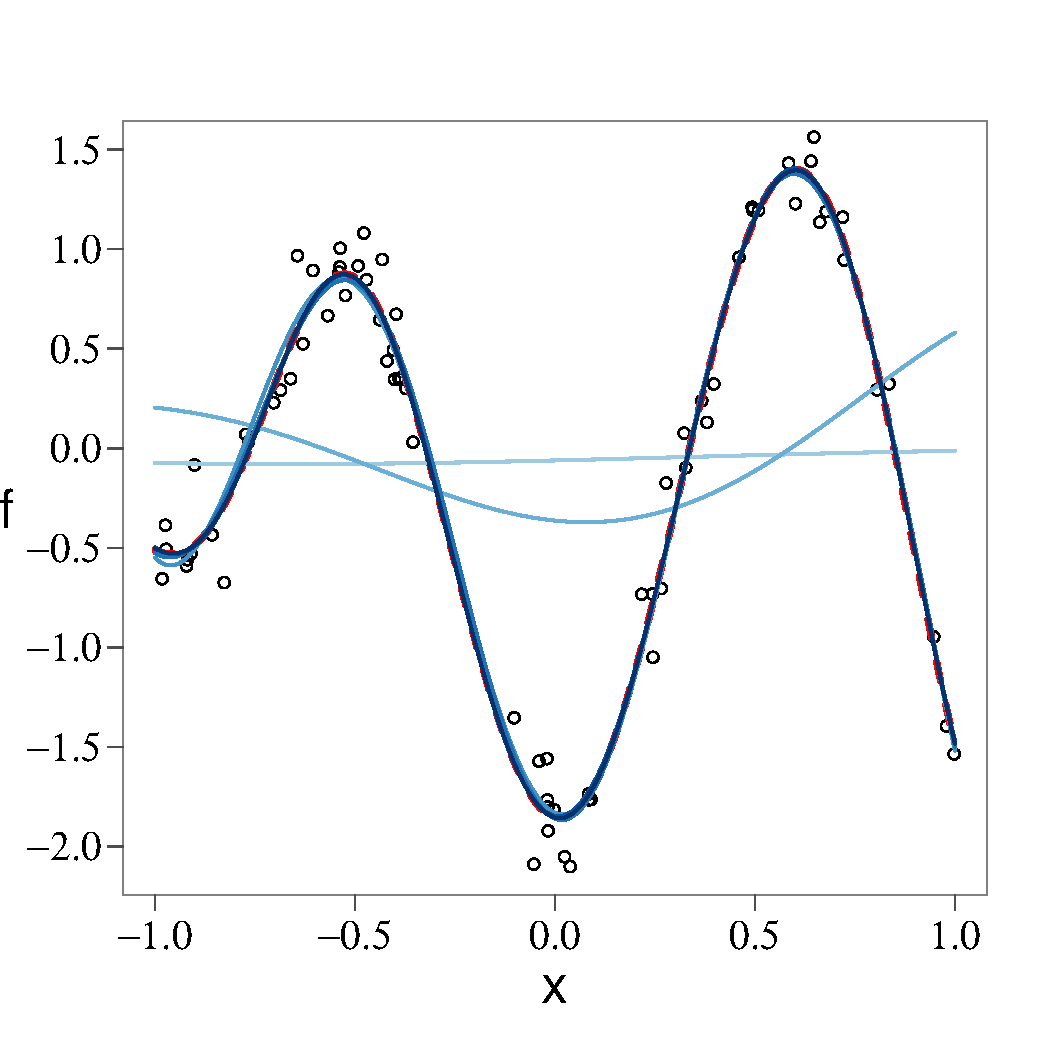
\includegraphics[scale=0.38, trim = 0mm 0mm 5mm 0mm, clip]{fig1_Post_J.pdf}}
\subfigure{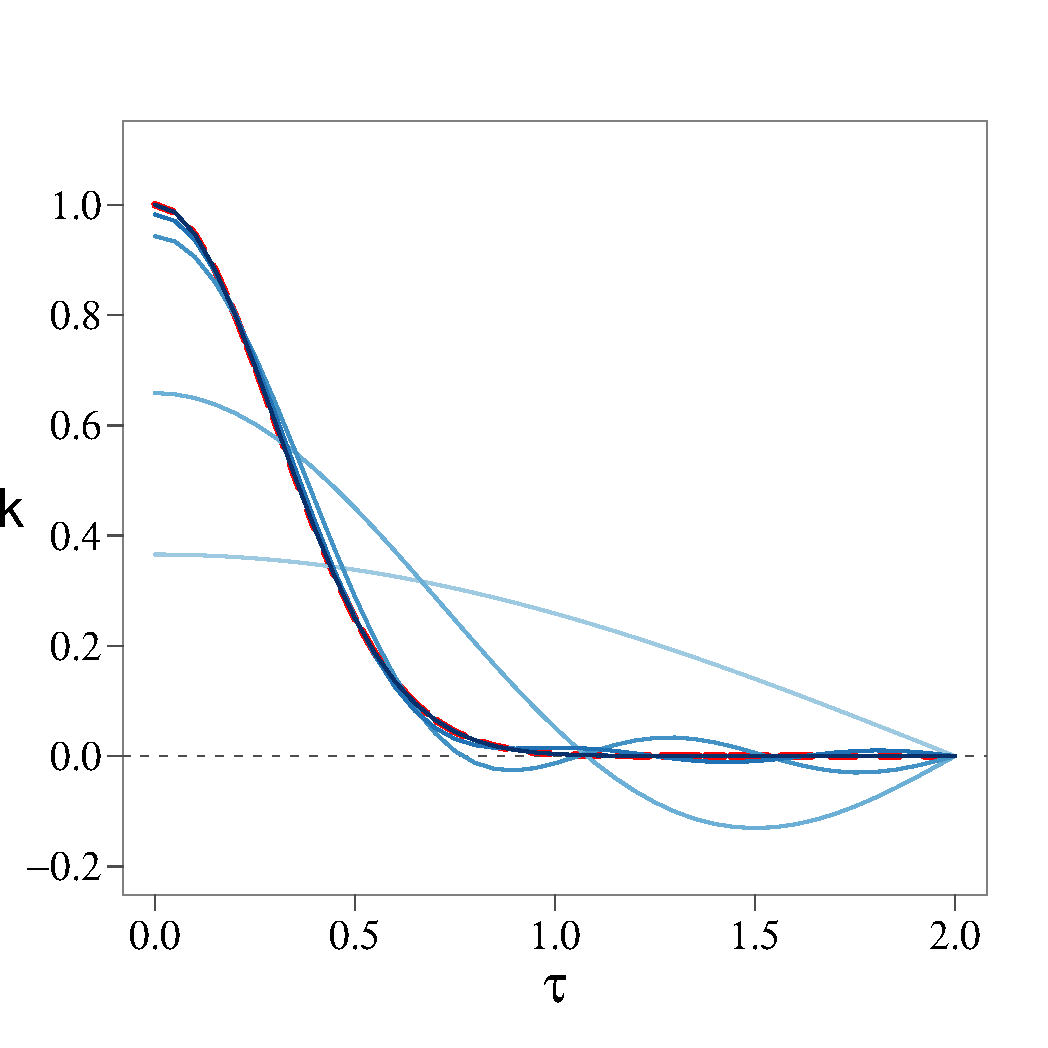
\includegraphics[scale=0.38, trim = 0mm 0mm 10mm 0mm, clip]{fig1_Cov_J.pdf}}
\subfigure{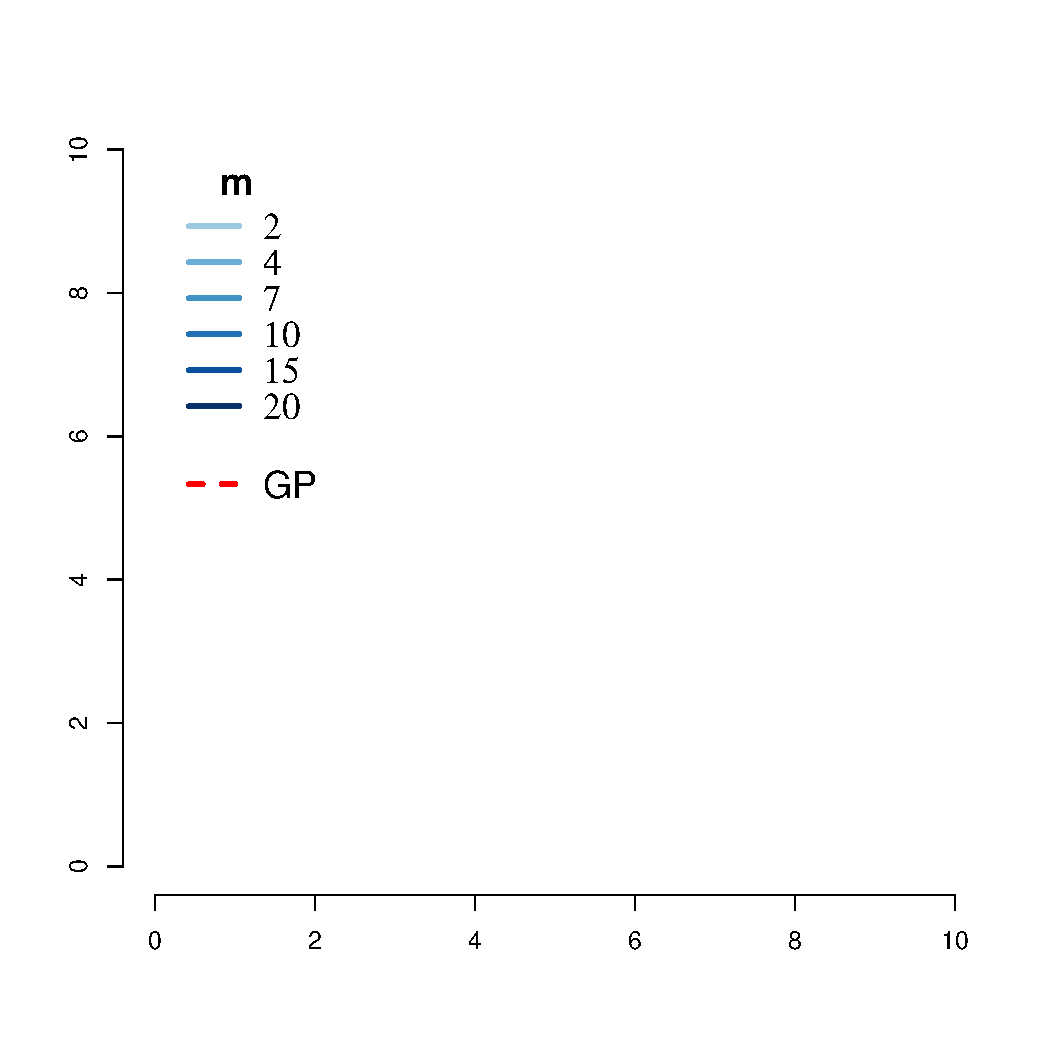
\includegraphics[scale=0.40, trim = 27mm 32mm 122mm 10mm, clip]{fig1_legend.pdf}}
\caption{Mean posterior predictive functions (left) and covariance functions (right) of both the regular GP model and the HSGP model for different number of basis functions $m$, with the boundary factor fixed to a large enough value.}
  \label{fig1_Post_J}
\end{figure}


\begin{figure}
\centering
\subfigure{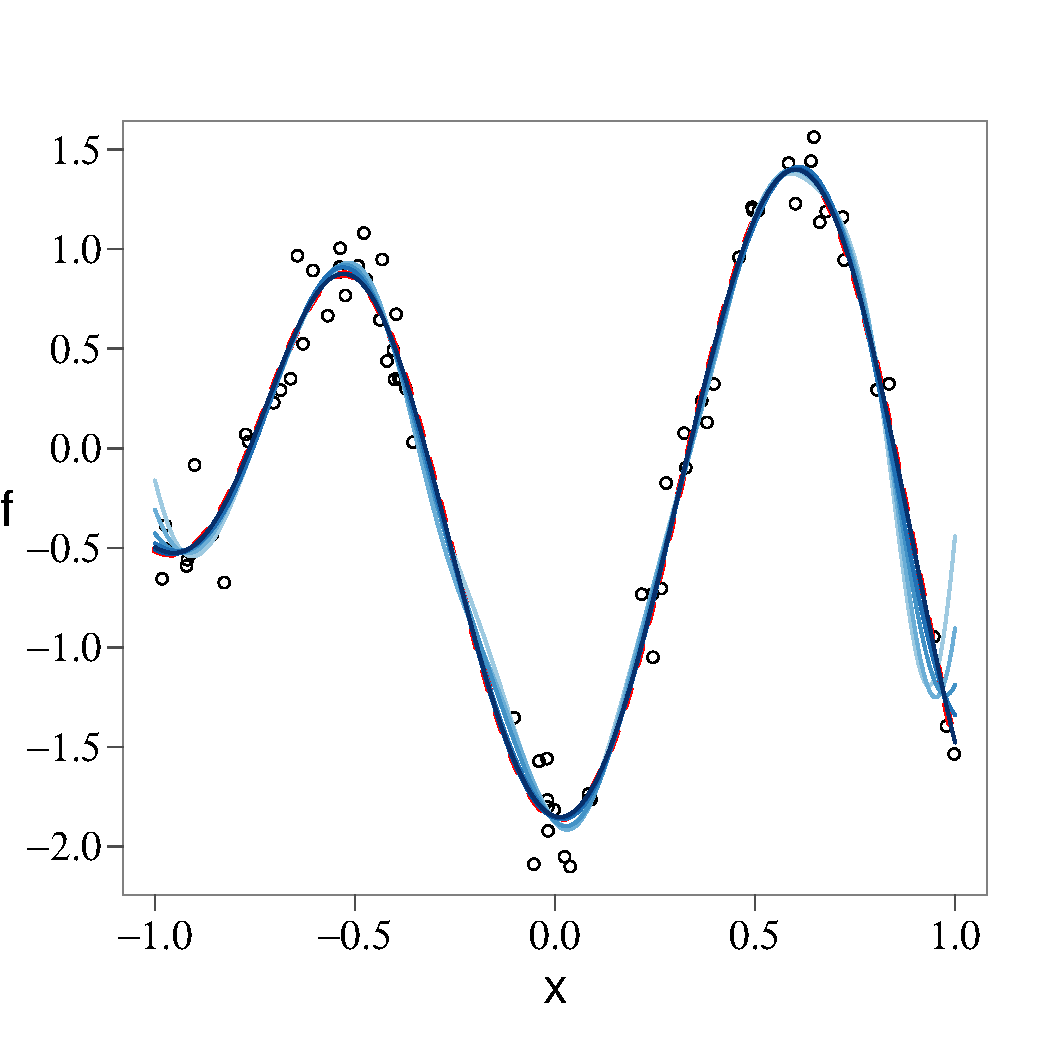
\includegraphics[scale=0.38, trim = 0mm 0mm 5mm 0mm, clip]{fig2_Post_L.pdf}}
\subfigure{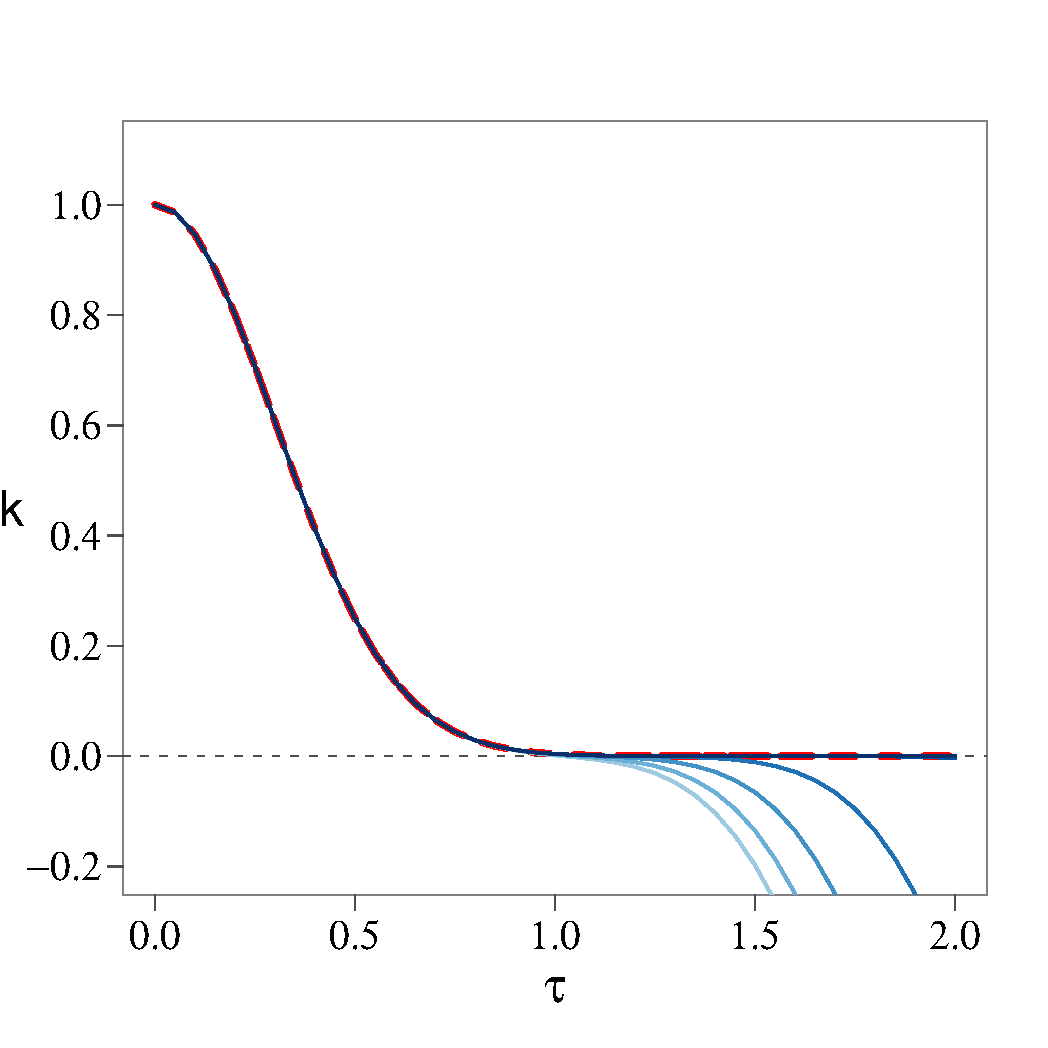
\includegraphics[scale=0.38, trim = 0mm 0mm 10mm 0mm, clip]{fig2_Cov_L.pdf}}
\subfigure{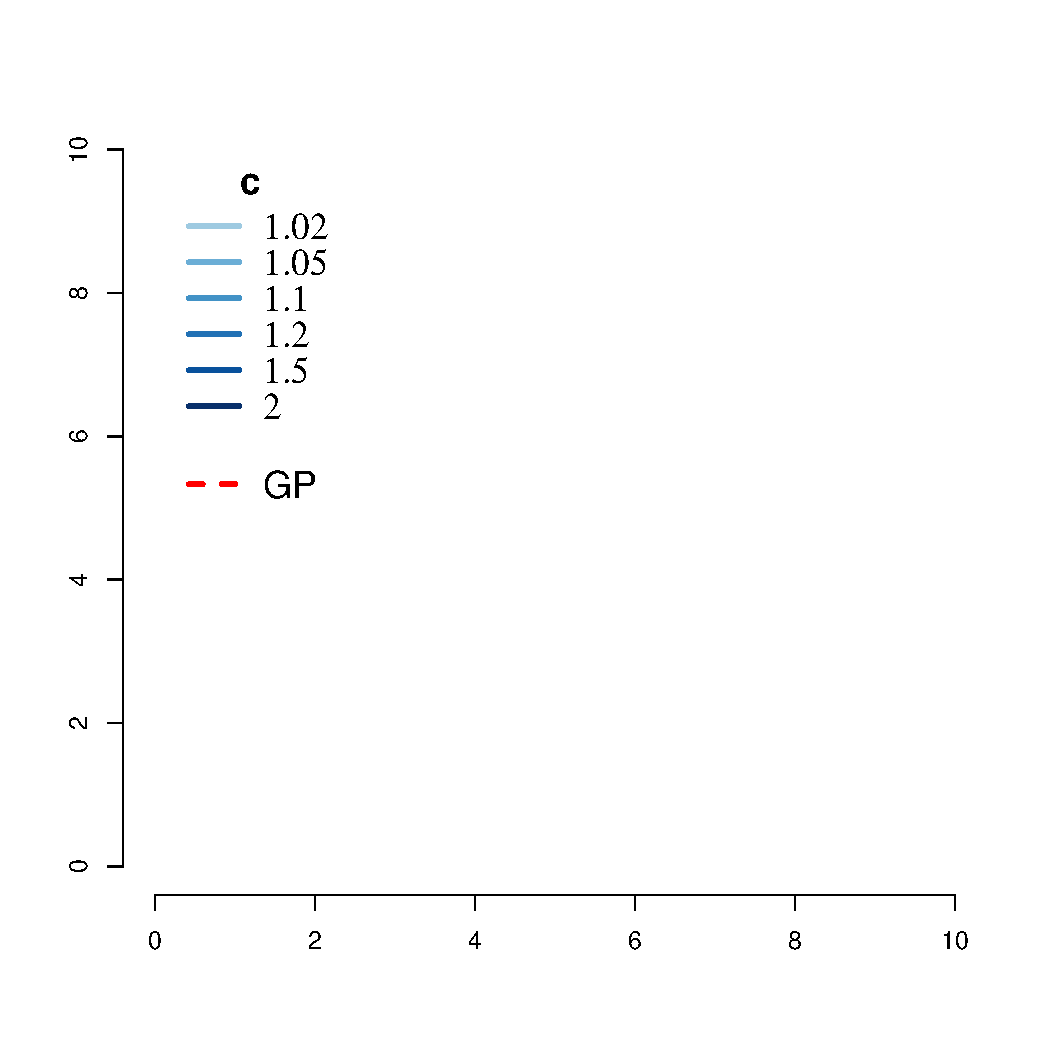
\includegraphics[scale=0.40, trim = 27mm 32mm 120mm 0mm, clip]{fig2_legend.pdf}}
\caption{Mean posterior predictive functions (left) and covariance functions (right) of both the regular GP model and the HSGP model for different values of the boundary factor $c$, with a large enough fixed number of basis functions.}
  \label{fig2_Post_L}
\end{figure}

Next, we will focus on analyzing the interaction effects between these $m$ and $c$ on the performance of the approximation. The lengthscale and marginal variance will no longer be fixed but rather estimated in both regular GP and HSGP models. Figure \ref{fig3_Post_part1} shows the functional posterior predictions and the covariance function obtained after fitting the data, for varying $m$ and $c$. Figure \ref{fig4_MSE_vs_J} shows the root mean square error (RMSE) of the HSGP models, computed against the regular GP model. Figure \ref{fig5_lscale_vs_J} shows the estimated lengthscale and marginal variance for the regular GP model and the HSGP models. Looking at the RMSEs in Figure \ref{fig4_MSE_vs_J}, we can conclude that the optimal choice in terms of precision and computations would be $m = 15$ basis functions and a boundary factor between $c = 1.5$ and $c = 2.5$. Further, the choice of $m = 10$ and $c = 1.5$ could still be an accurate enough choice. We may also come to the same conclusion by looking at the posterior predictions and covariance function plots in Figure \ref{fig3_Post_part1}. From these results, some general conclusions may be drawn:

\begin{itemize}
\item As $c$ increases, $m$ has to increase as well (and vice versa).
\item There exists a minimum $c$ below which a close approximation will never be achieved regardless of $m$.
\end{itemize}

\begin{figure}
\begin{center}
\begin{tabular}{| c | c | c | c |}
\hline
c  = 1.05 & 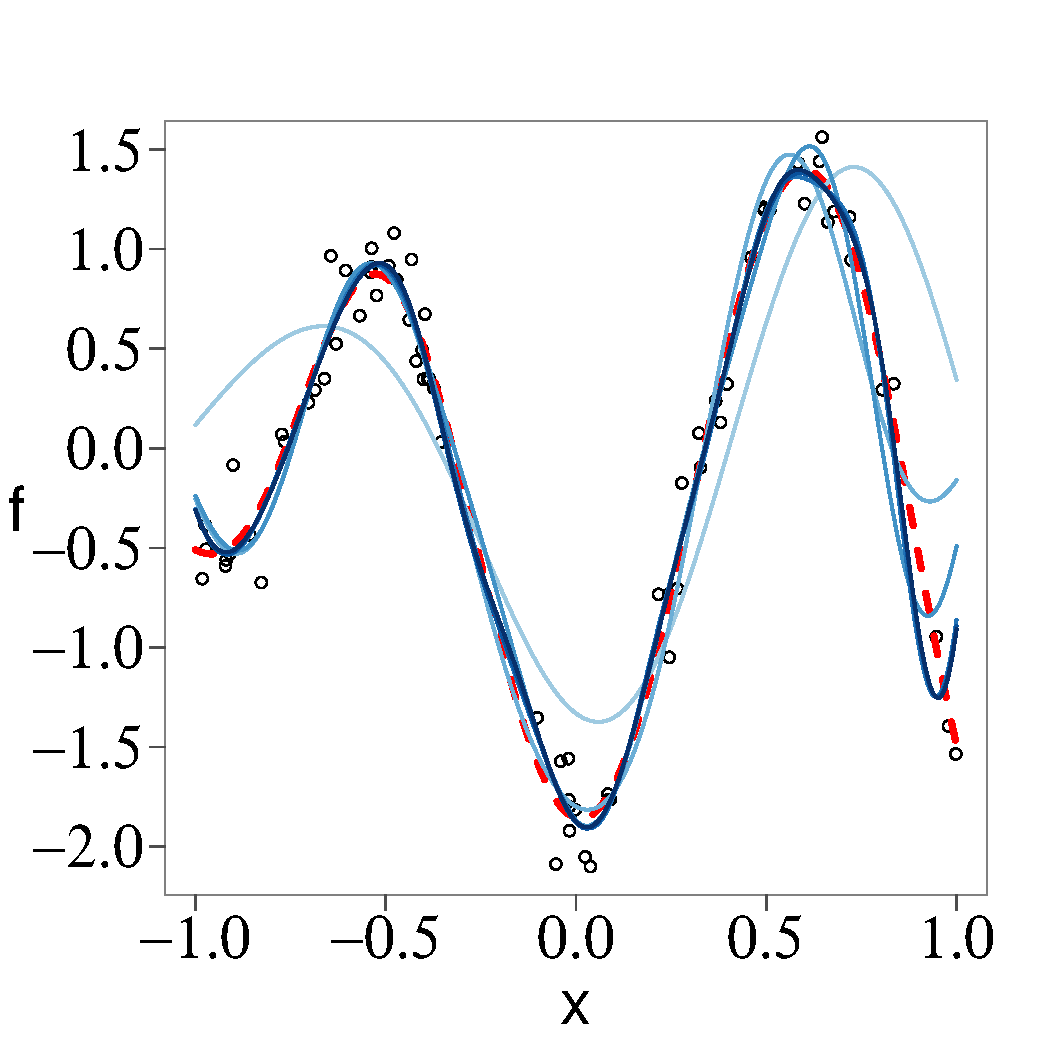
\includegraphics[scale=0.23, trim = 0mm 14mm 0mm 14mm, clip]{fig3_Post_part1.pdf} & 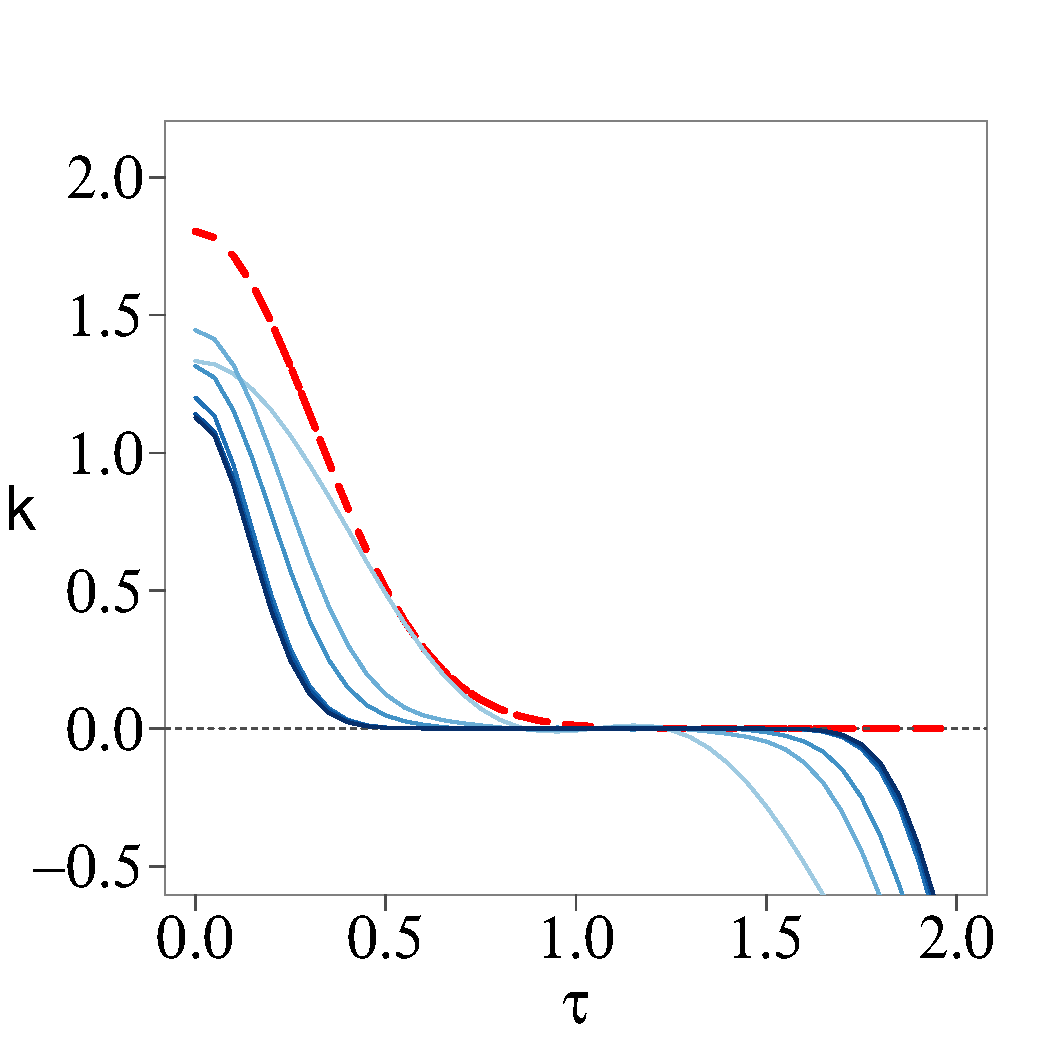
\includegraphics[scale=0.23, trim = 0mm 14mm 0mm 14mm, clip]{fig3_Cov_part1.pdf} & \multirow{36}{1.3cm}{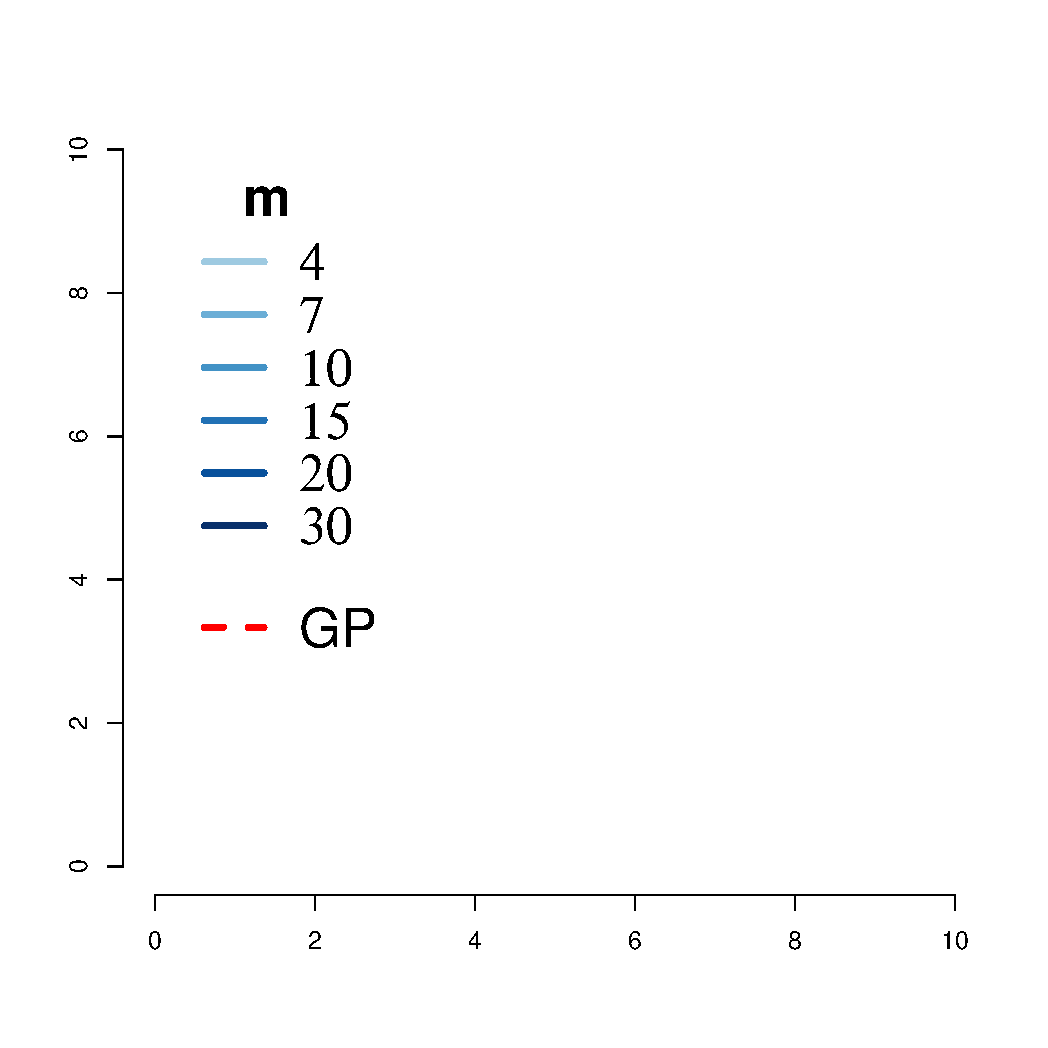
\includegraphics[scale=0.35, trim = 28mm 40mm 100mm 30mm, clip]{fig3_legend.pdf}}\\ 
\cline{1-3}
c  = 1.1 & 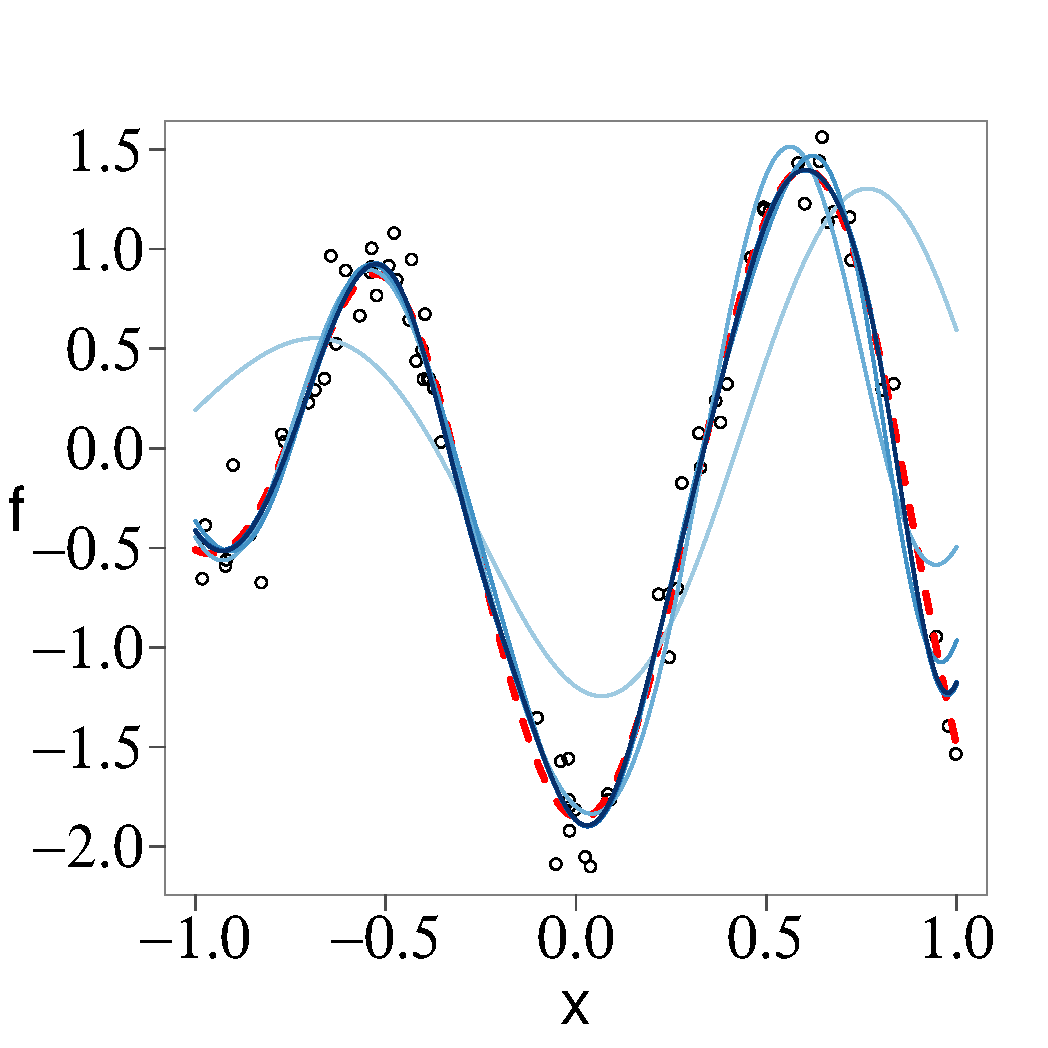
\includegraphics[scale=0.23, trim = 0mm 14mm 0mm 14mm, clip]{fig3_Post_part2.pdf} & 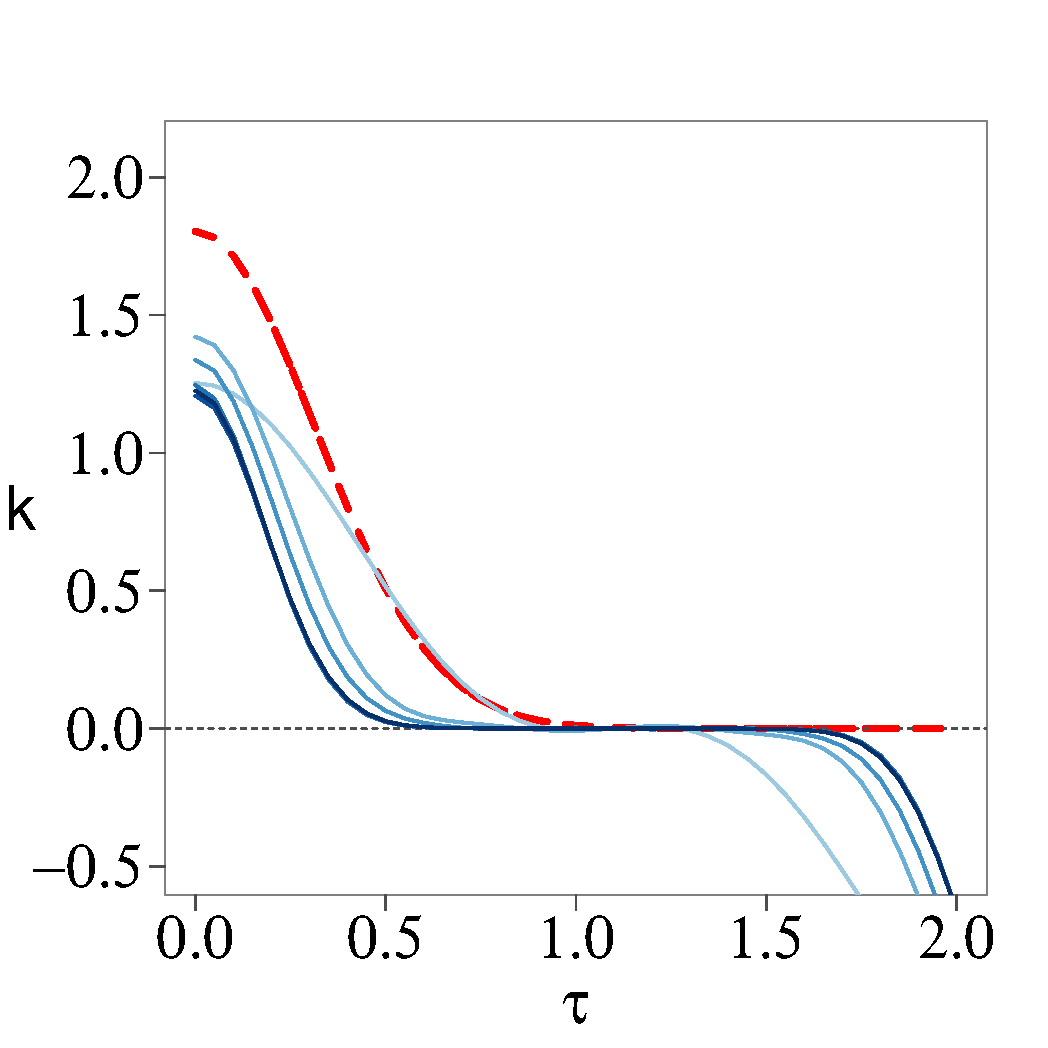
\includegraphics[scale=0.23, trim = 0mm 14mm 0mm 14mm, clip]{fig3_Cov_part2.pdf} &\\
\cline{1-3}
c  = 1.2 & 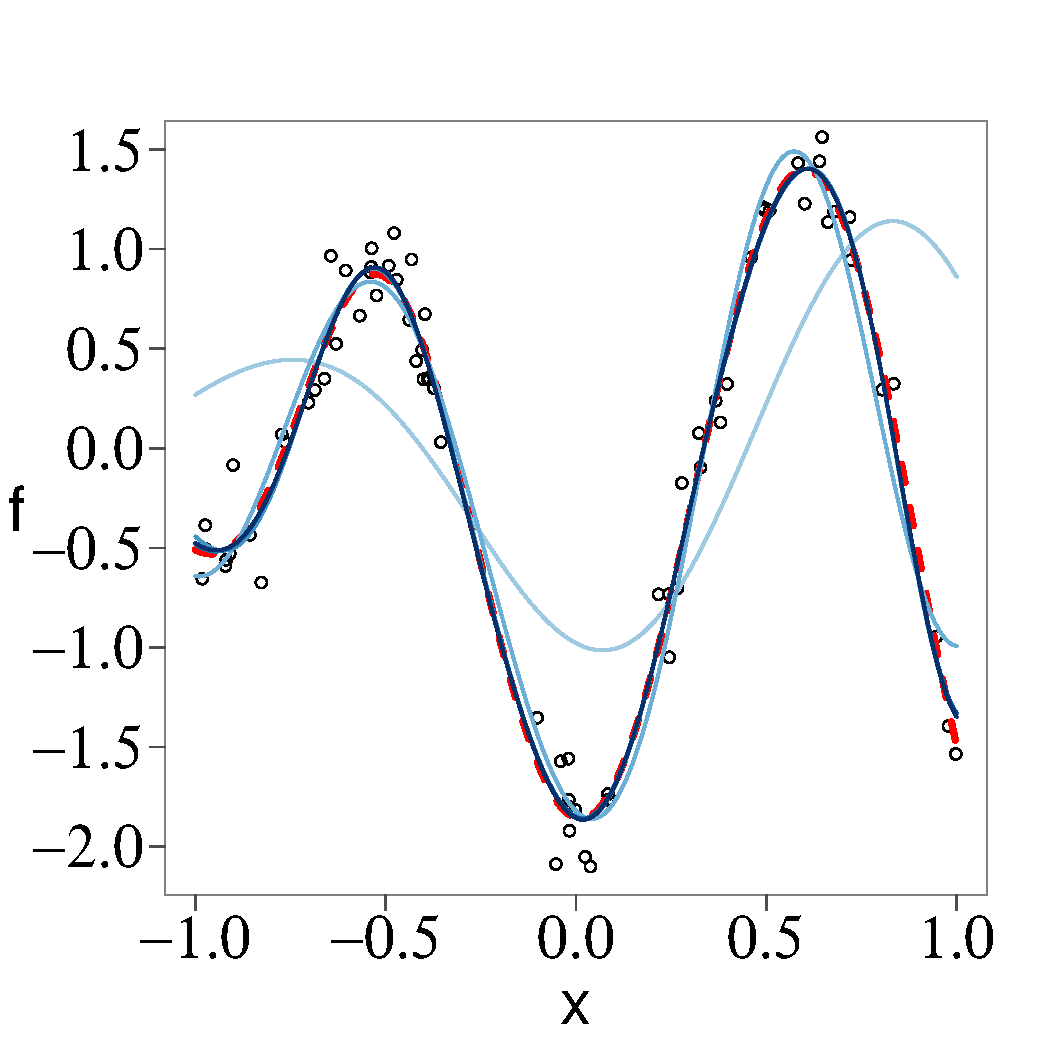
\includegraphics[scale=0.23, trim = 0mm 14mm 0mm 14mm, clip]{fig3_Post_part3.pdf} & 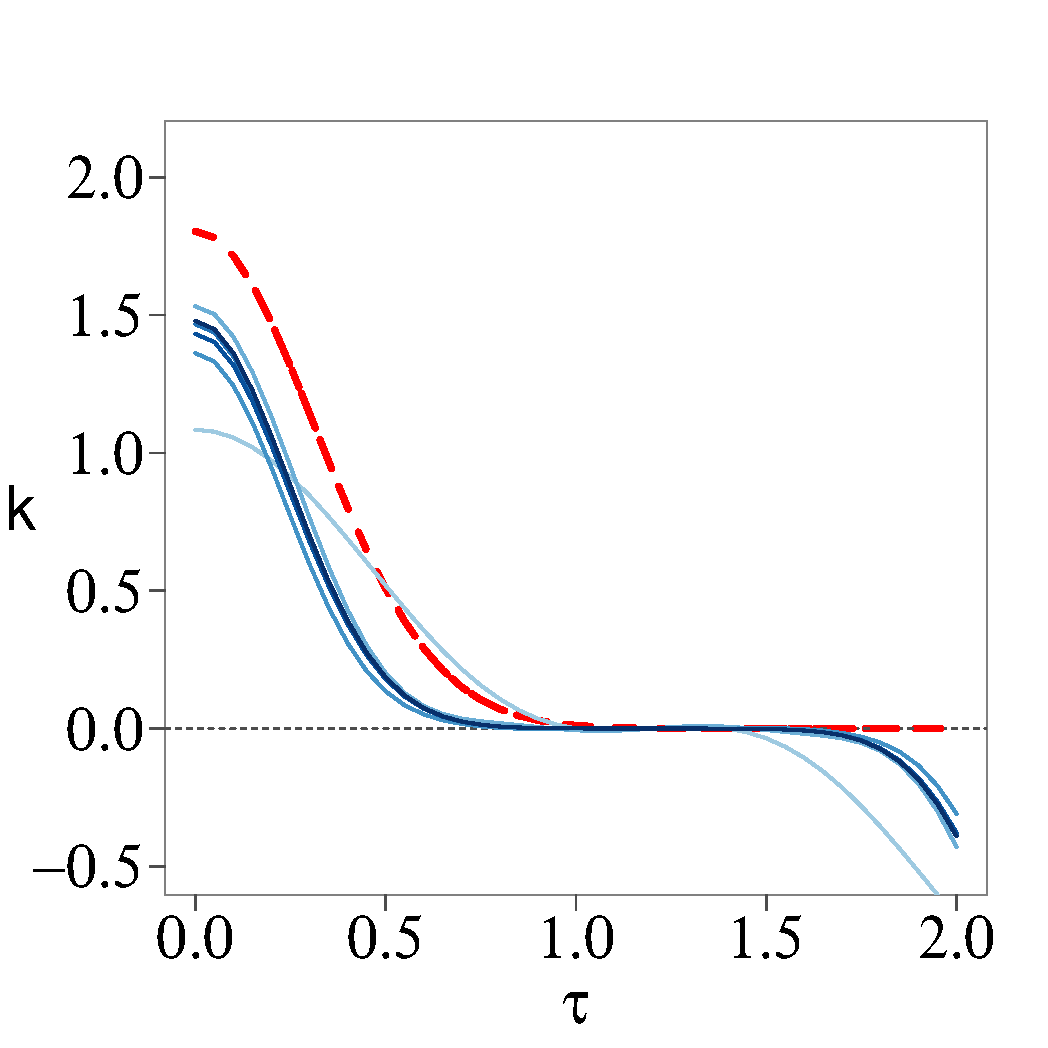
\includegraphics[scale=0.23, trim = 0mm 14mm 0mm 14mm, clip]{fig3_Cov_part3.pdf} &\\
\cline{1-3}
c  = 1.5 & 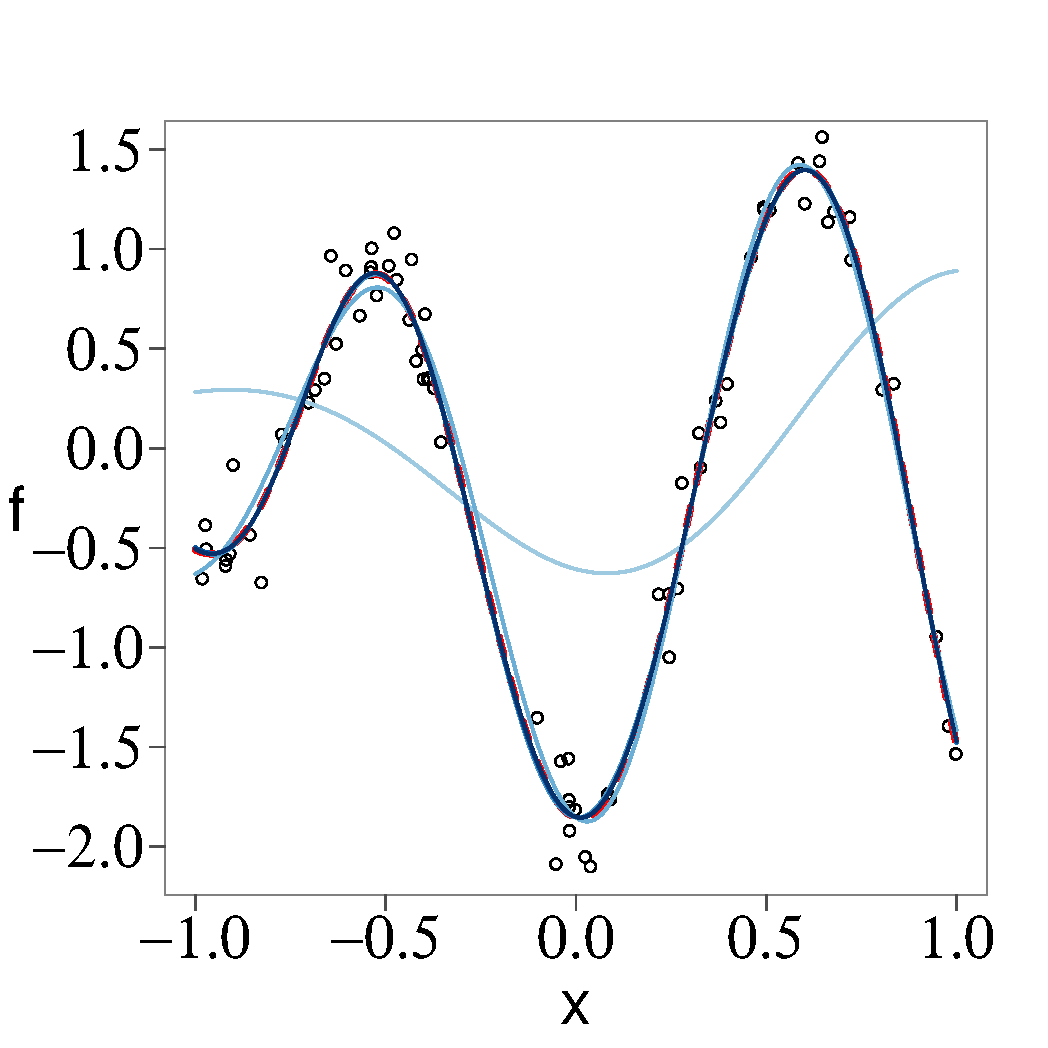
\includegraphics[scale=0.23, trim = 0mm 14mm 0mm 14mm, clip]{fig3_Post_part4.pdf} & 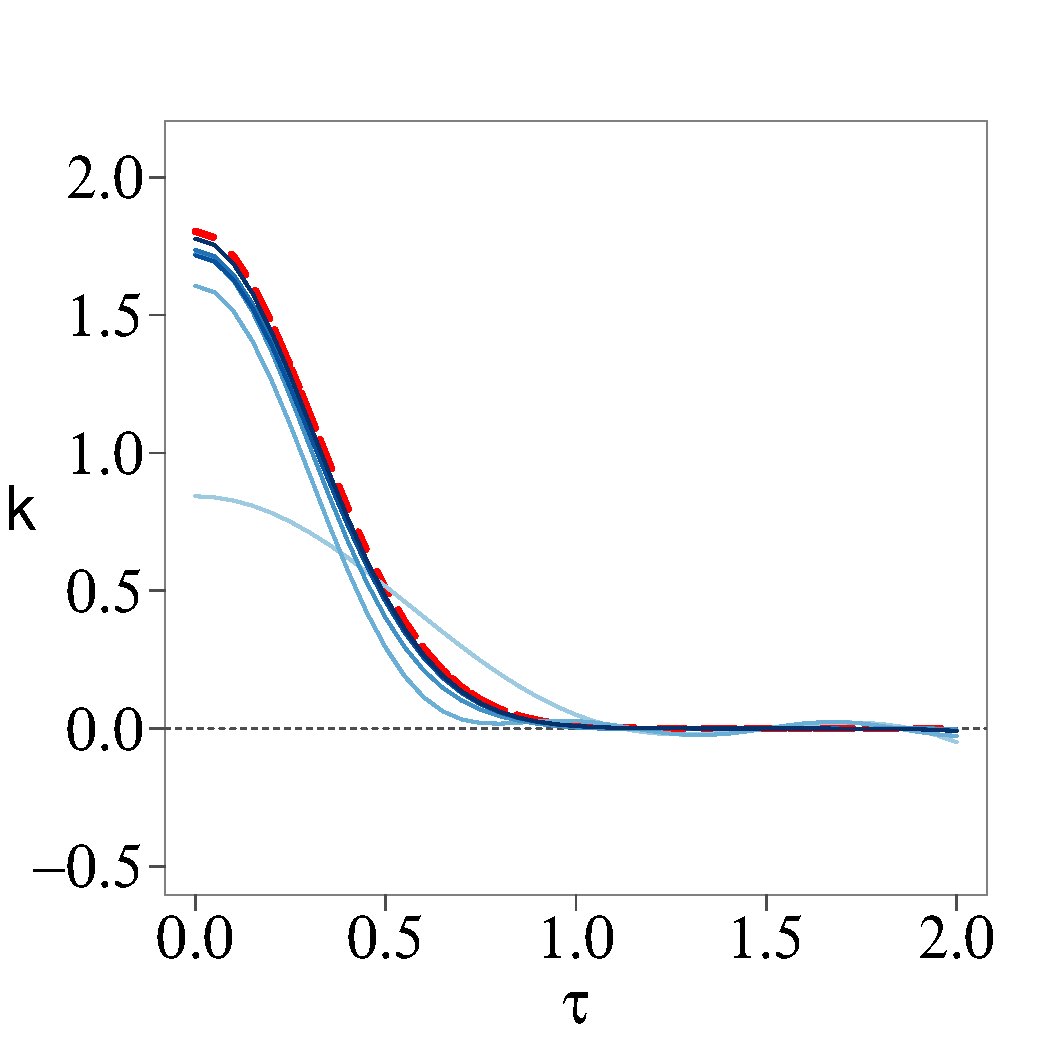
\includegraphics[scale=0.23, trim = 0mm 14mm 0mm 14mm, clip]{fig3_Cov_part4.pdf} & \\
\cline{1-3}
c  = 2 & 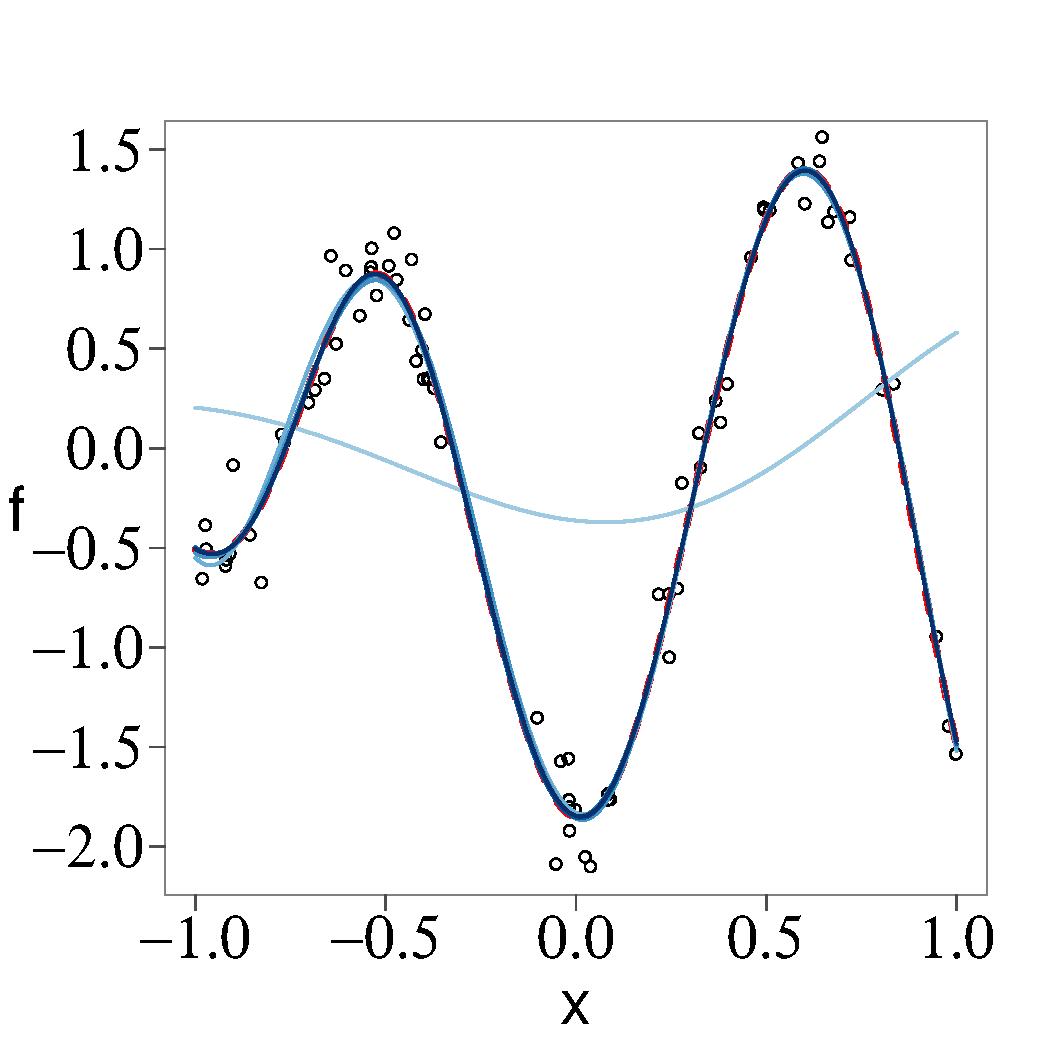
\includegraphics[scale=0.23, trim = 0mm 14mm 0mm 14mm, clip]{fig3_Post_part5.pdf} &  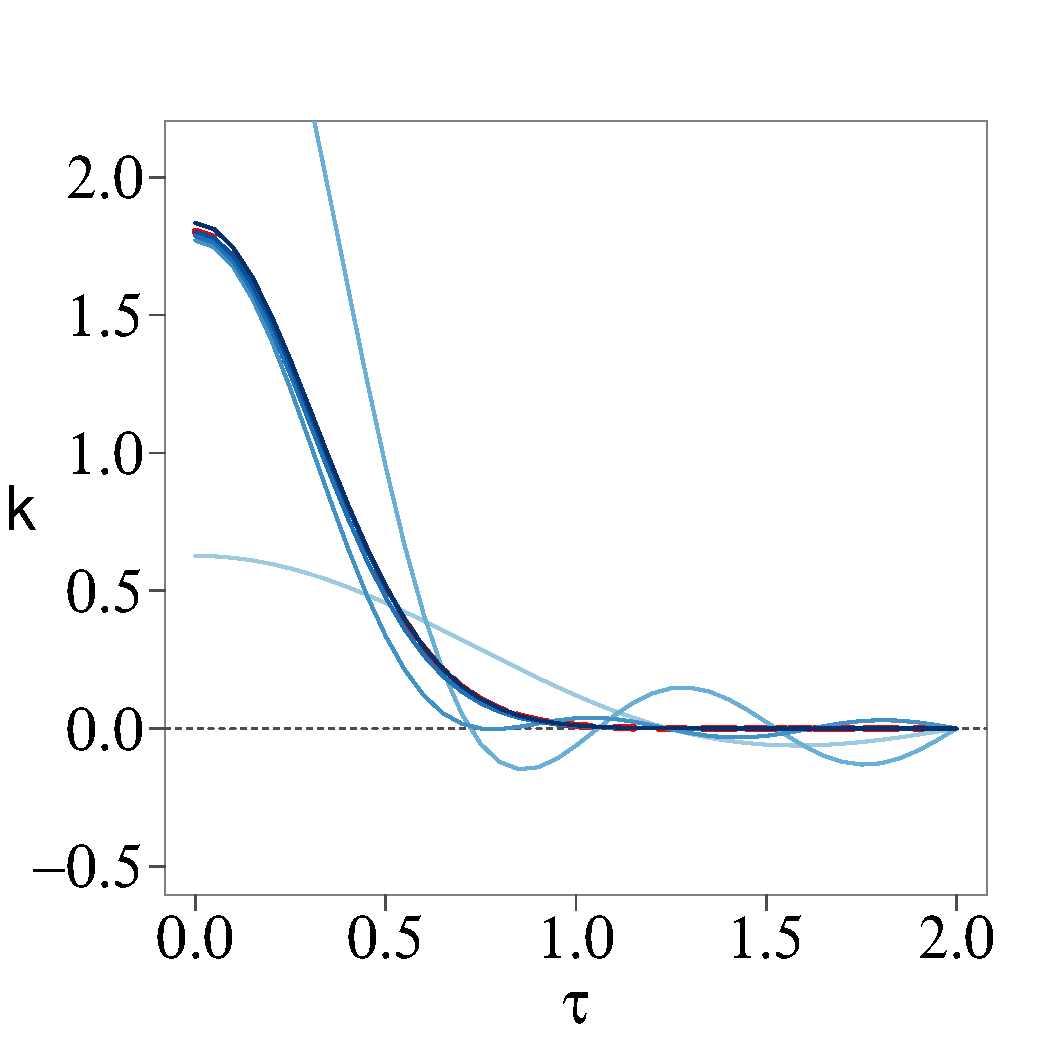
\includegraphics[scale=0.23, trim = 0mm 14mm 0mm 14mm, clip]{fig3_Cov_part5.pdf} &\\
\cline{1-3}
c  = 2.5 & 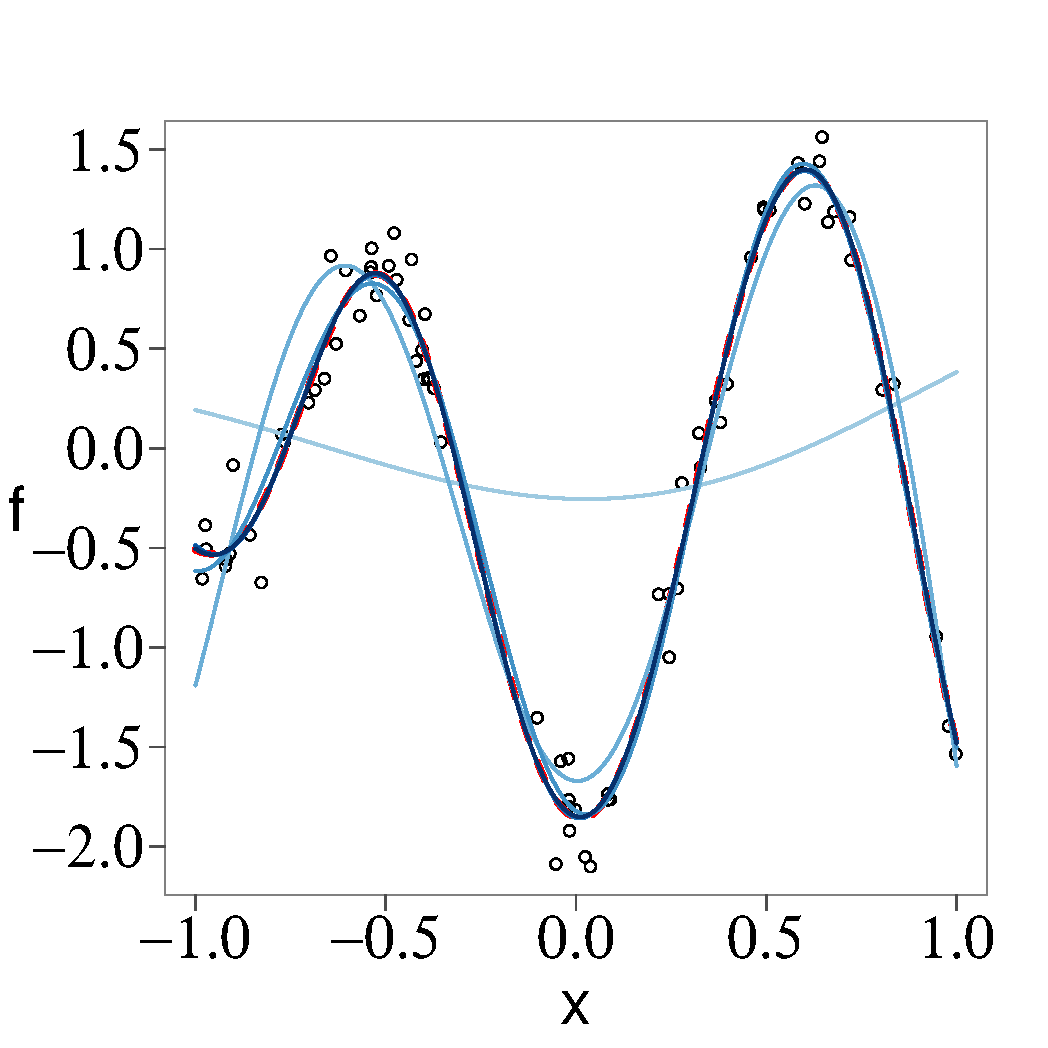
\includegraphics[scale=0.23, trim = 0mm 4mm 0mm 14mm, clip]{fig3_Post_part6.pdf} & 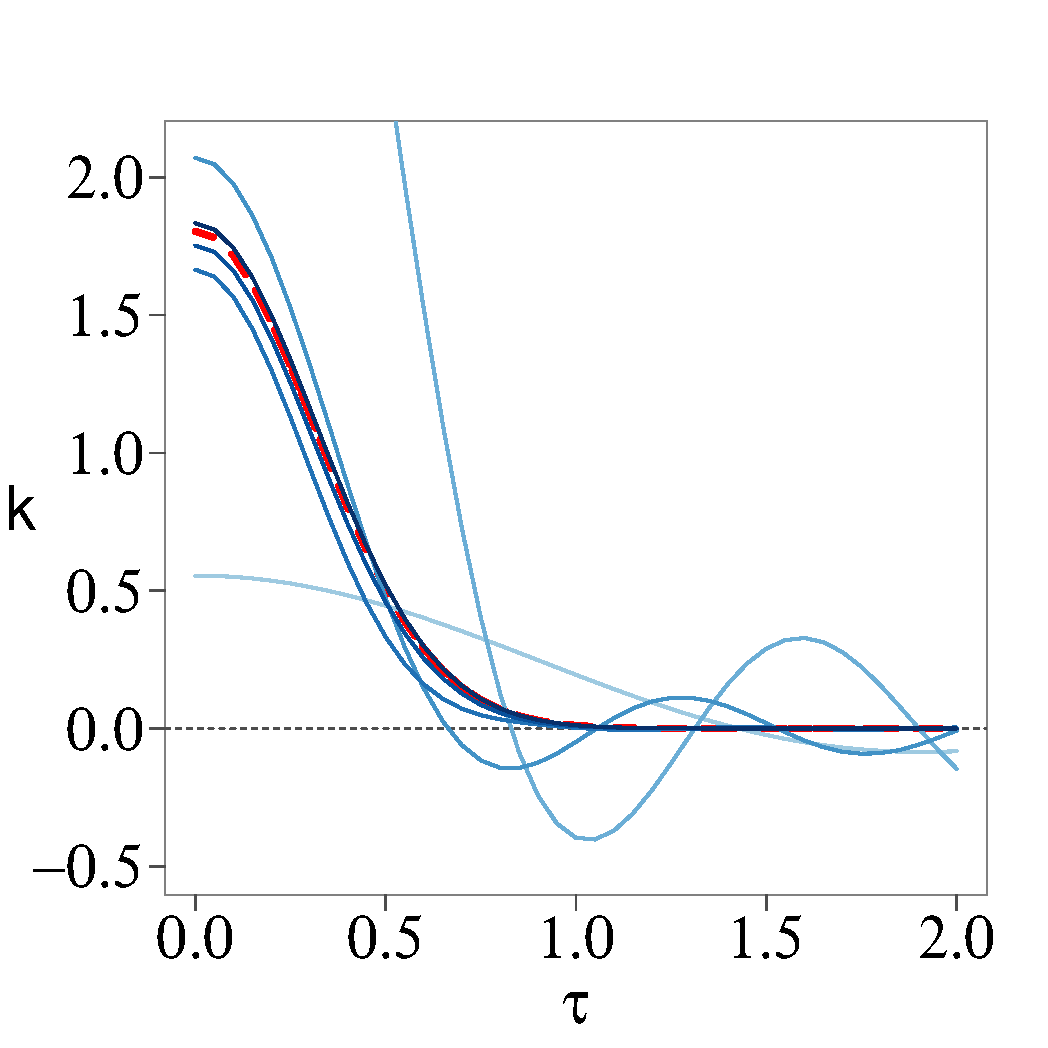
\includegraphics[scale=0.23, trim = 0mm 4mm 0mm 14mm, clip]{fig3_Cov_part6.pdf} &\\
\hline
\end{tabular}
\end{center}
\caption{Mean posterior predictive functions (left) and covariance functions (right) of both the regular GP model and the HSGP model for different number of basis functions $m$ and for different values of the boundary factor $c$.}
  \label{fig3_Post_part1}
\end{figure}

%\begin{figure}
%\begin{tabular}{ c c c c c}
%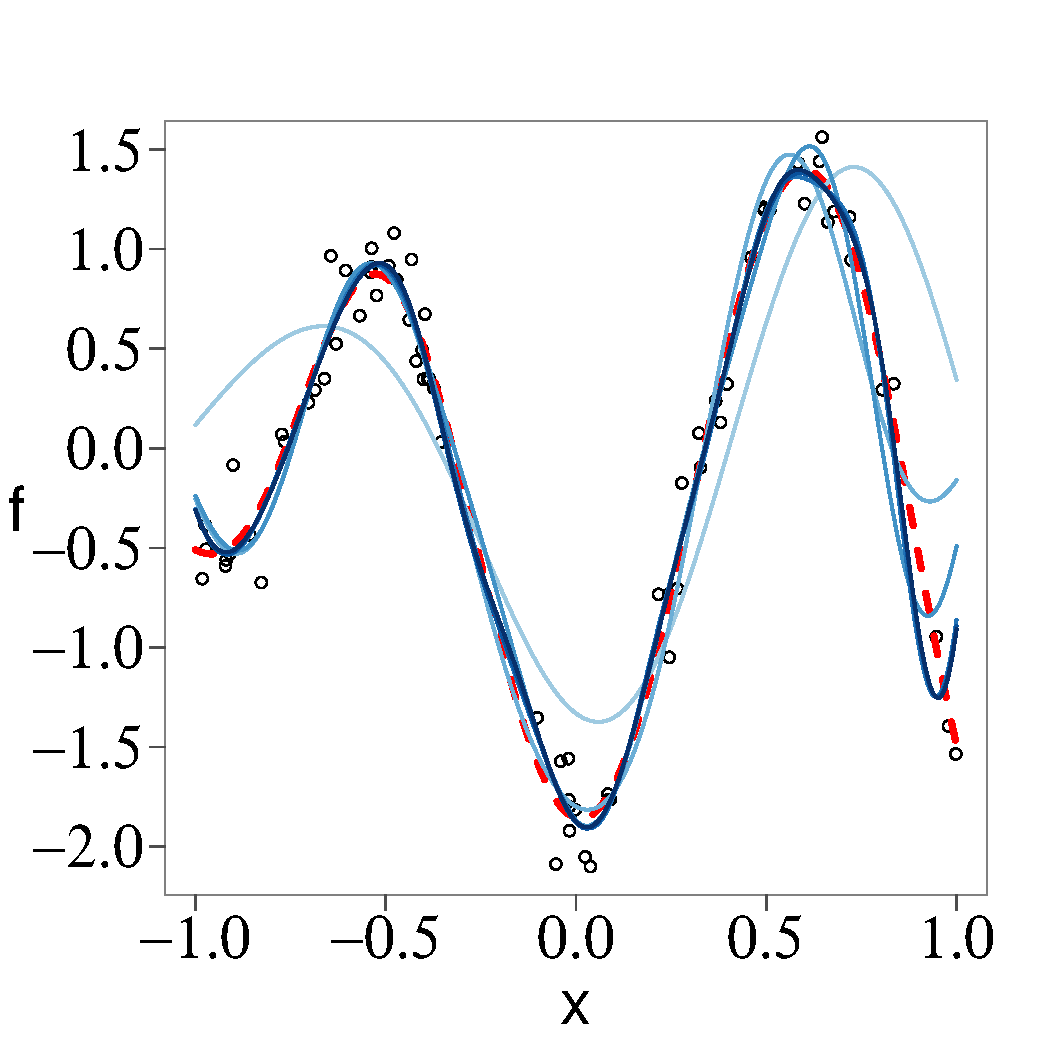
\includegraphics[scale=0.20, trim = 10mm 24mm 10mm 20mm, clip]{fig3_Post_part1.pdf} & \hspace{-5mm} 
%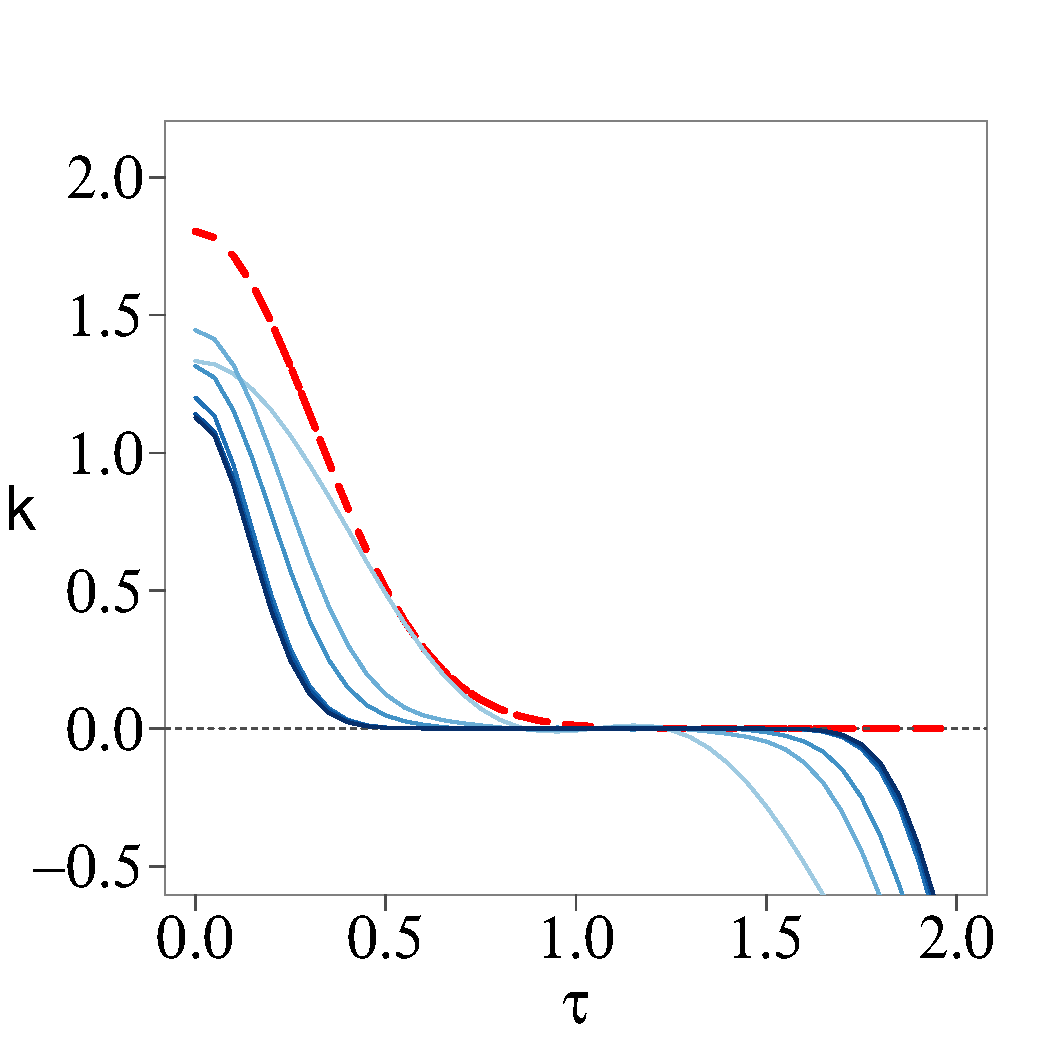
\includegraphics[scale=0.20, trim = 5mm 24mm 10mm 20mm, clip]{fig3_Cov_part1.pdf} &  \hspace{-0mm}
%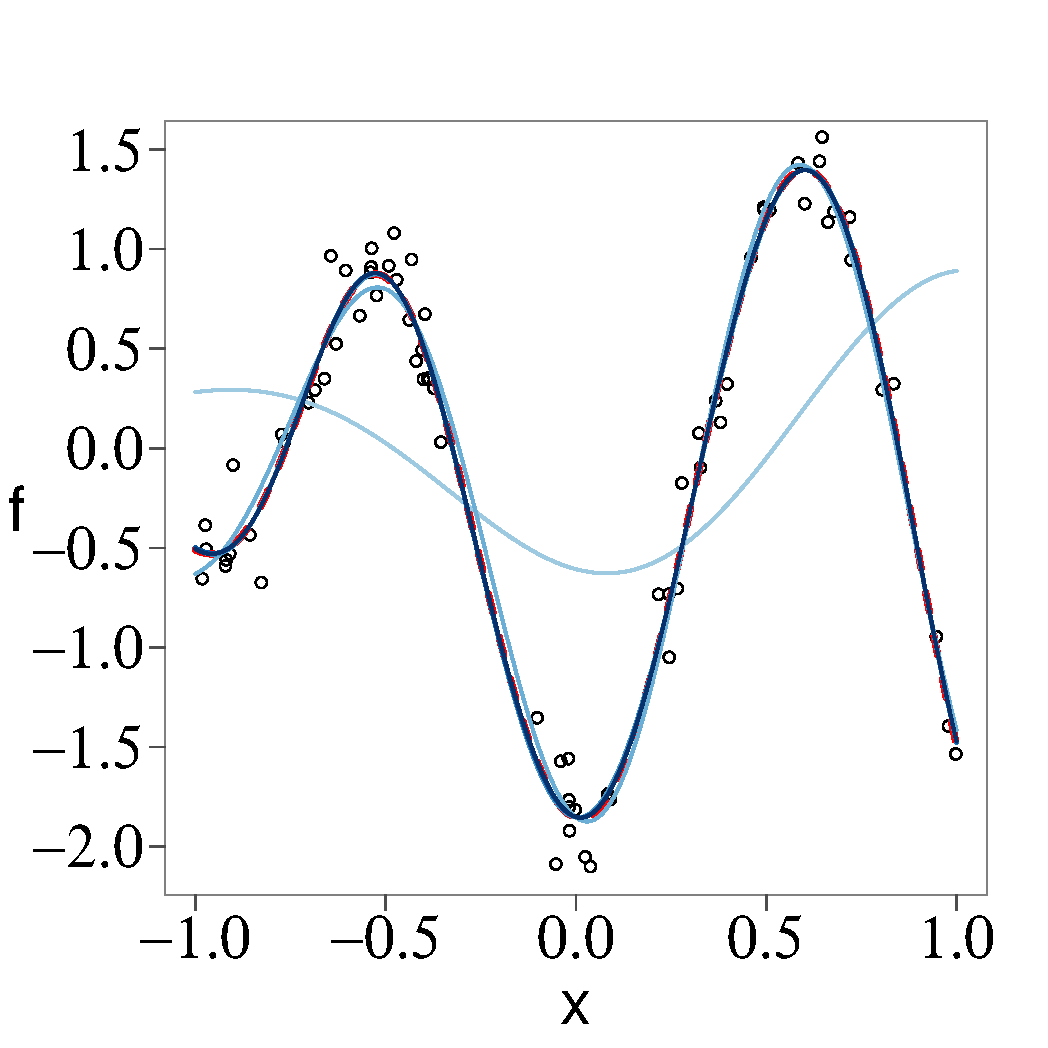
\includegraphics[scale=0.20, trim = 5mm 24mm 10mm 20mm, clip]{fig3_Post_part4.pdf} & \hspace{-5mm} 
%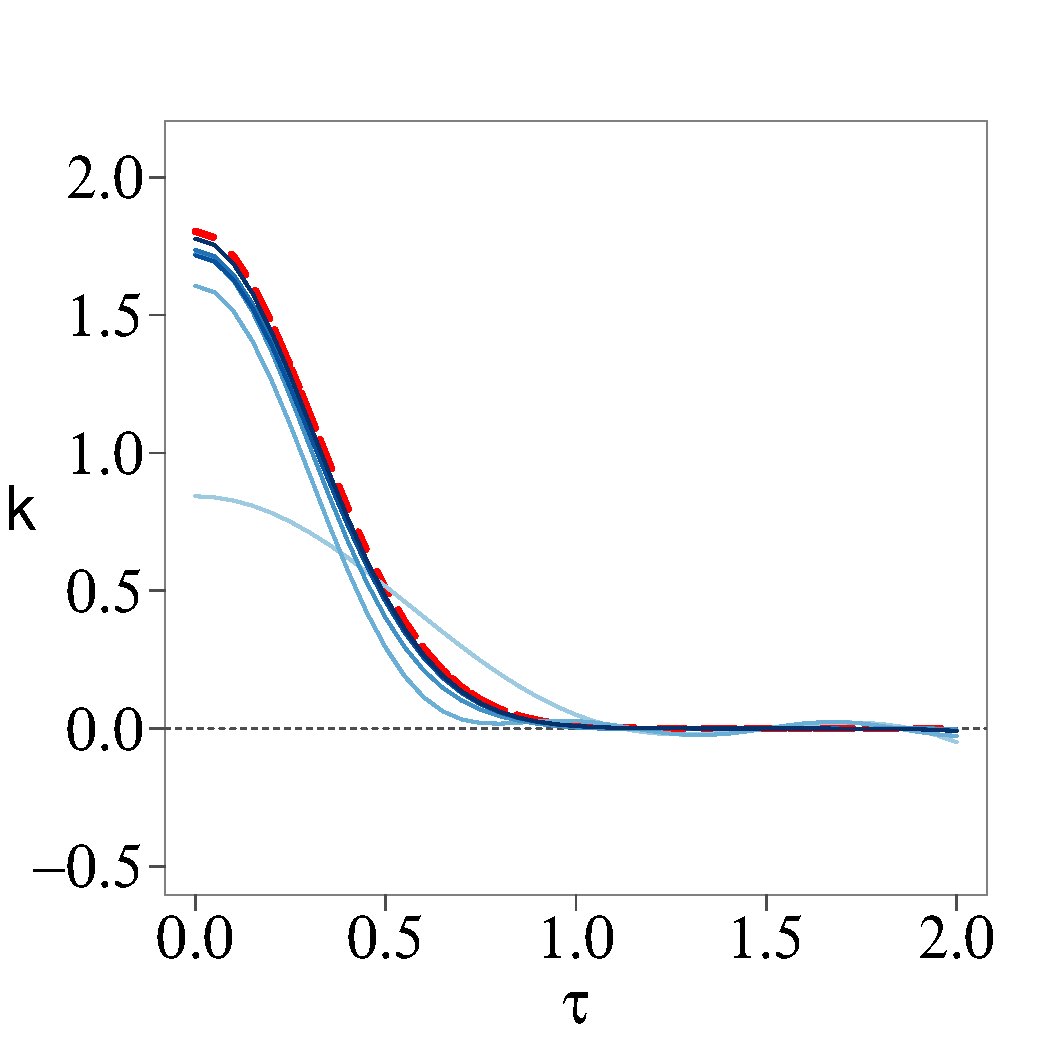
\includegraphics[scale=0.20, trim = 5mm 24mm 10mm 20mm, clip]{fig3_Cov_part4.pdf} & \\ 
%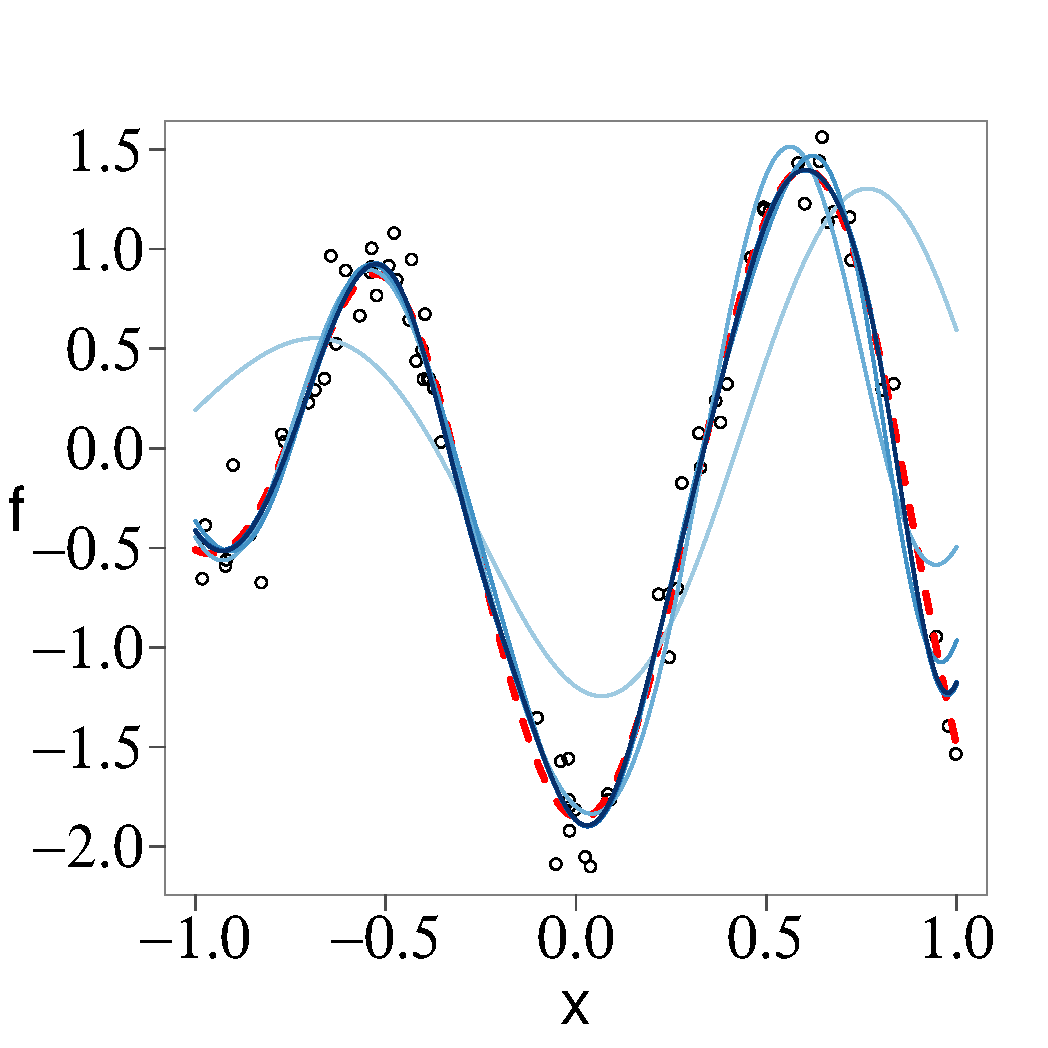
\includegraphics[scale=0.20, trim = 10mm 24mm 10mm 20mm, clip]{fig3_Post_part2.pdf} & \hspace{-5mm} 
%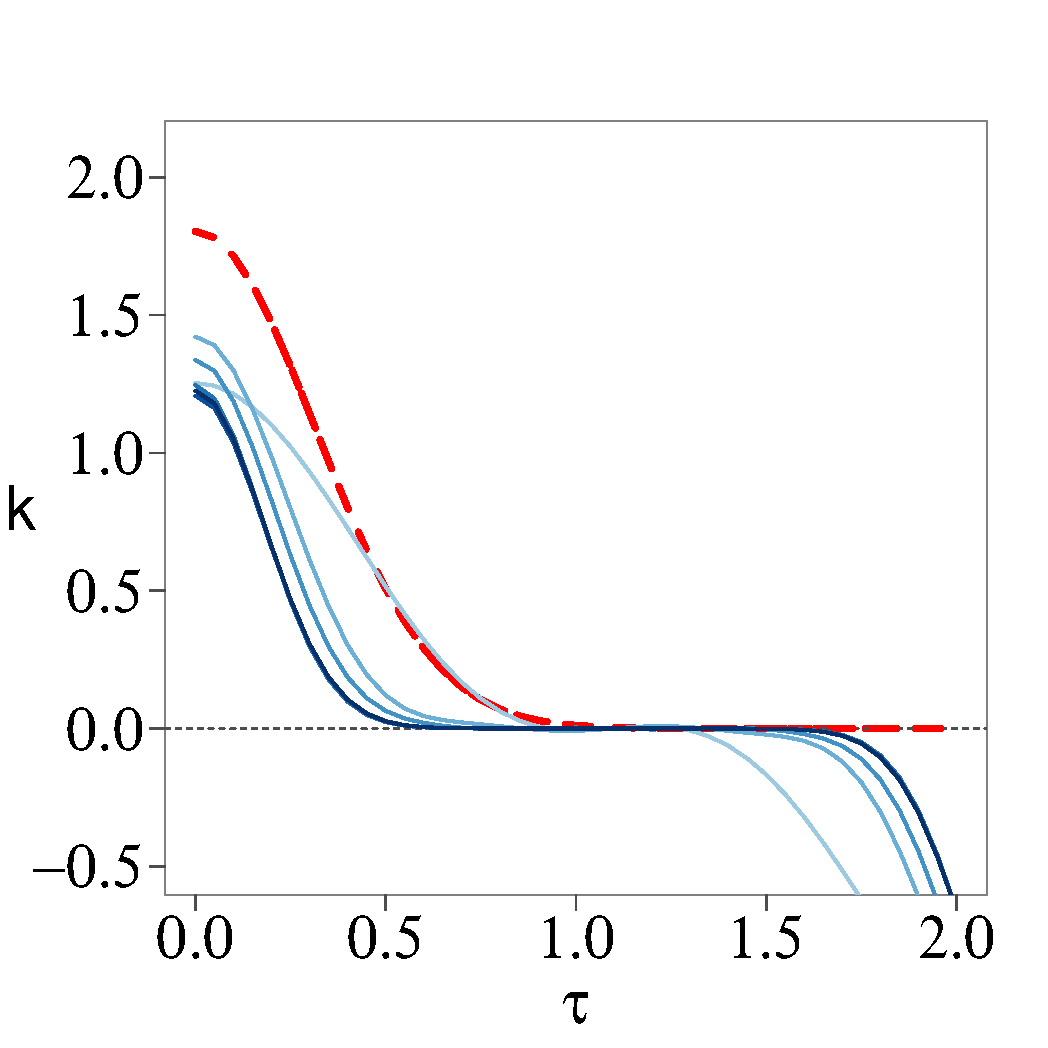
\includegraphics[scale=0.20, trim = 5mm 24mm 10mm 20mm, clip]{fig3_Cov_part2.pdf} & \hspace{-0mm}
%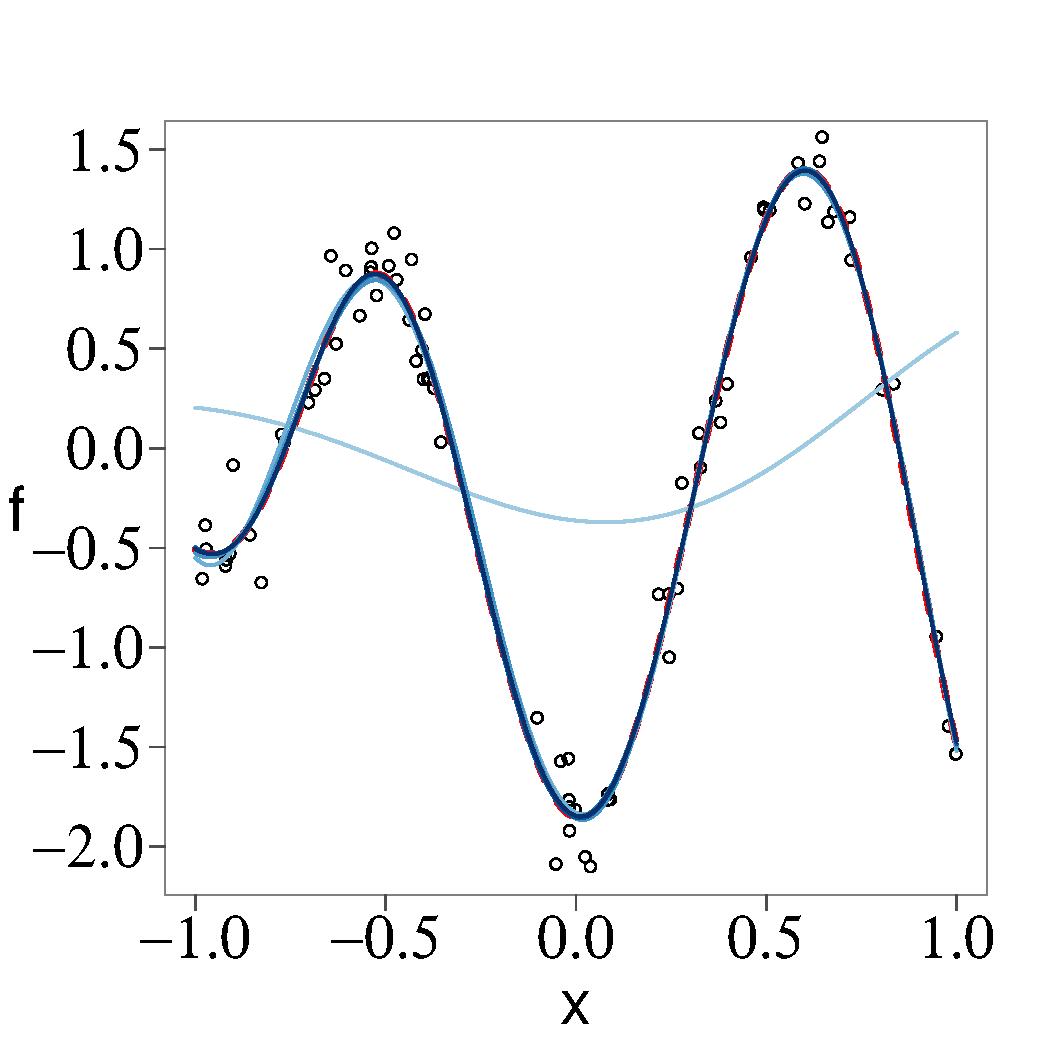
\includegraphics[scale=0.20, trim = 5mm 24mm 10mm 20mm, clip]{fig3_Post_part5.pdf} & \hspace{-5mm} 
%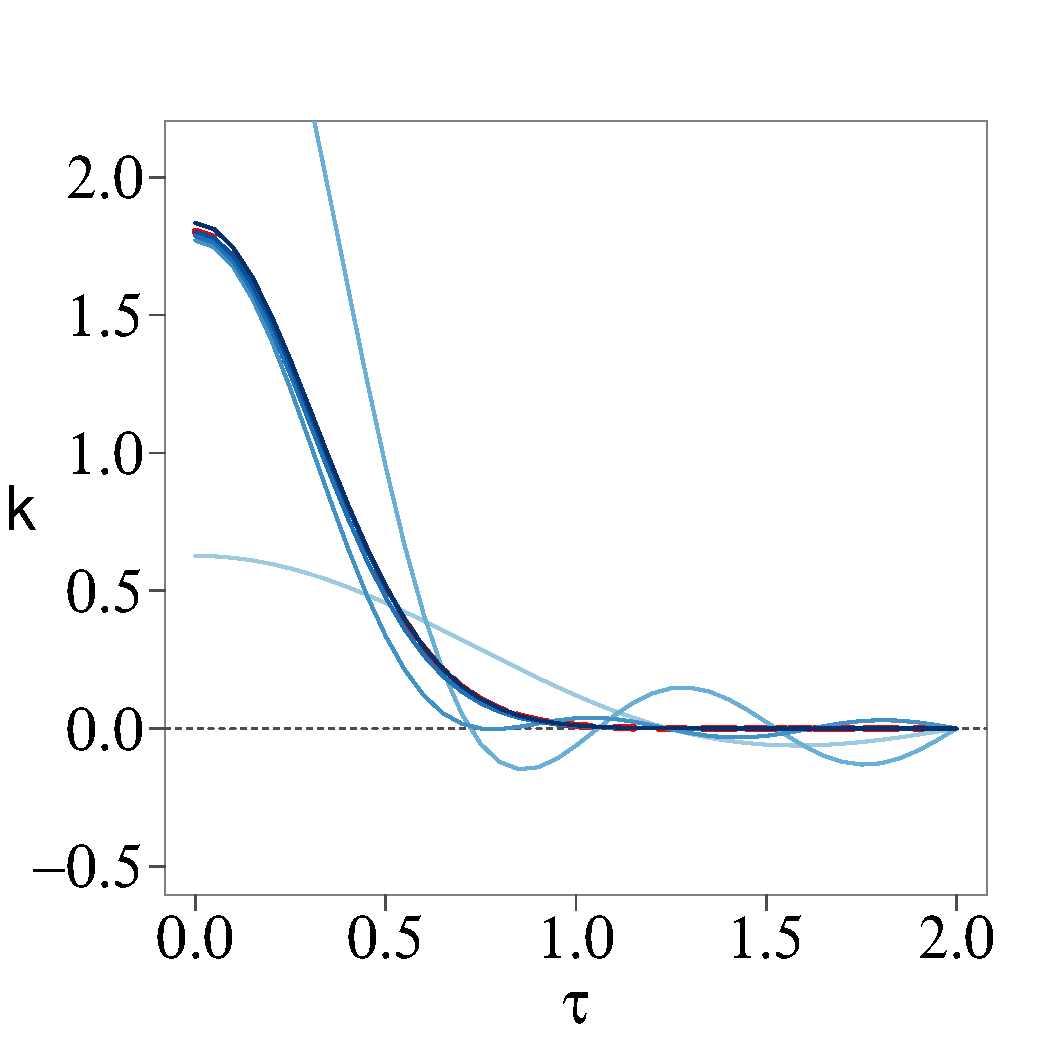
\includegraphics[scale=0.20, trim = 5mm 24mm 10mm 20mm, clip]{fig3_Cov_part5.pdf} & \hspace{-5mm} 
%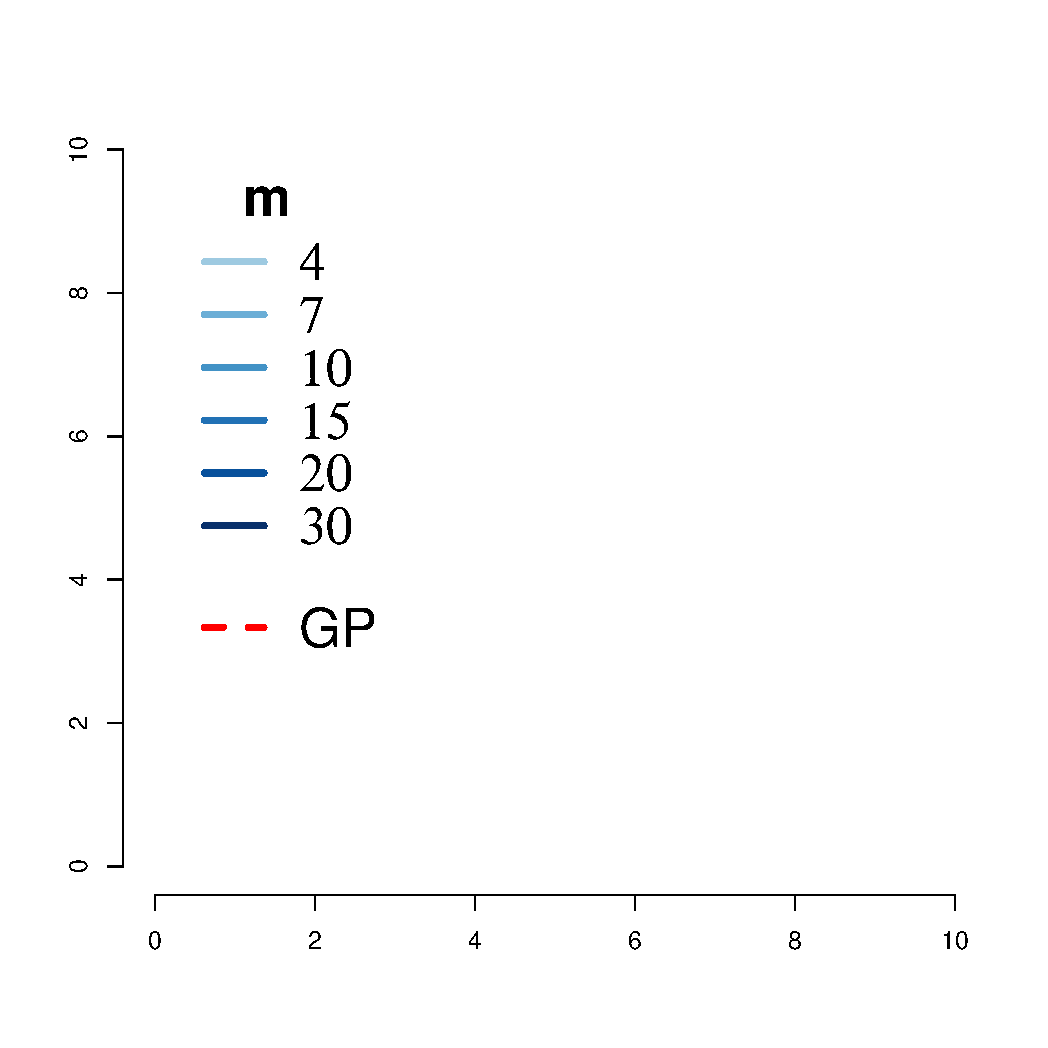
\includegraphics[scale=0.35, trim = 25mm 63mm 120mm 50mm, clip]{fig3_legend.pdf}\\
%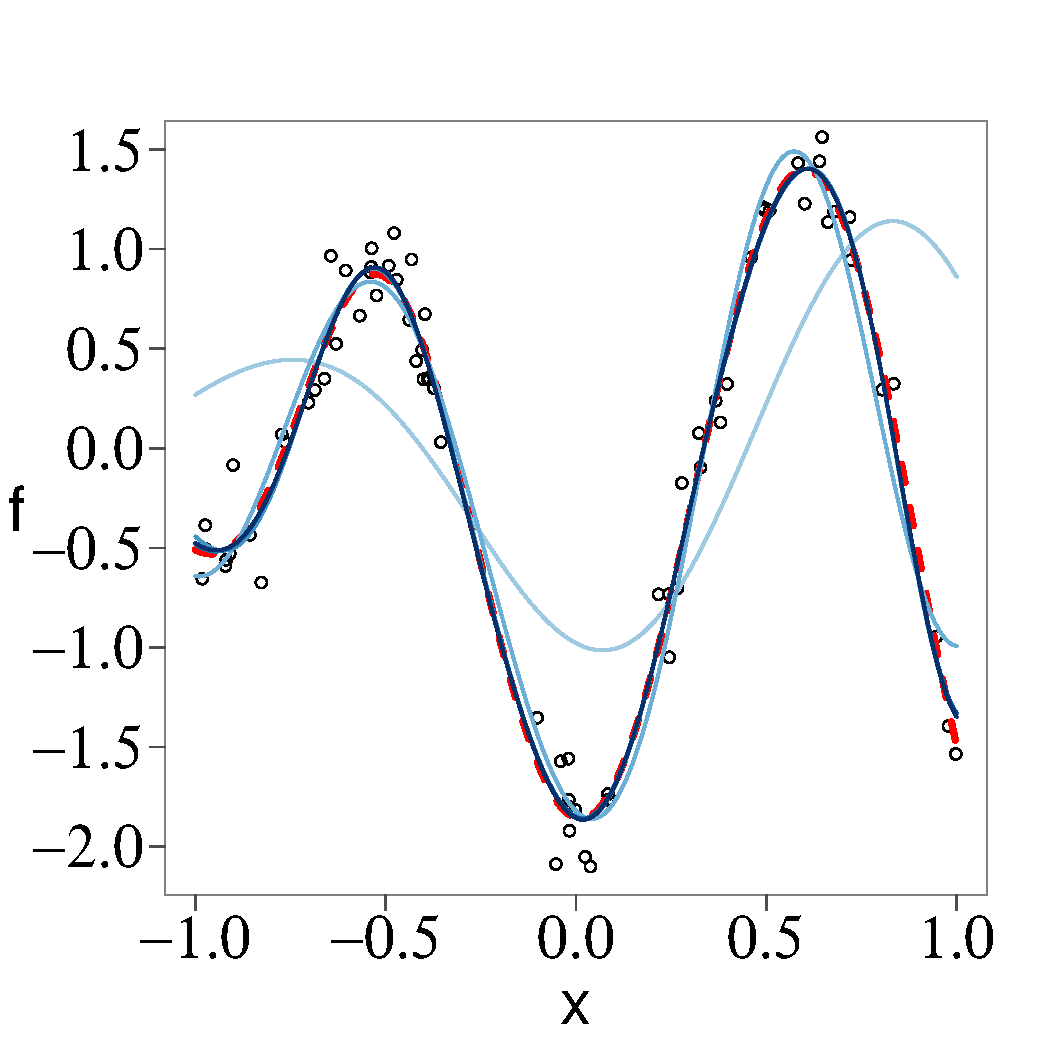
\includegraphics[scale=0.20, trim = 10mm 5mm 10mm 20mm, clip]{fig3_Post_part3.pdf} & \hspace{-5mm} 
%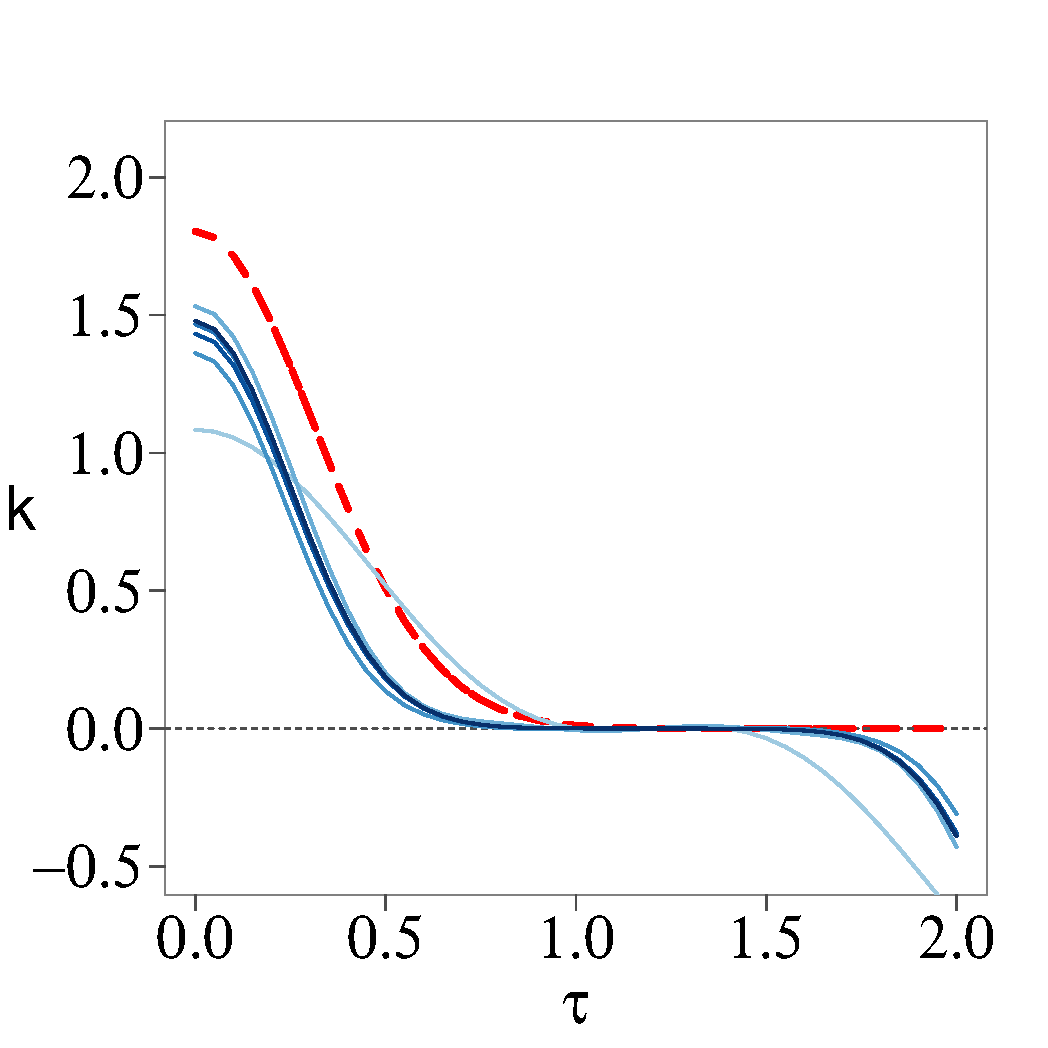
\includegraphics[scale=0.20, trim = 5mm 5mm 10mm 20mm, clip]{fig3_Cov_part3.pdf} & \hspace{-0mm}
%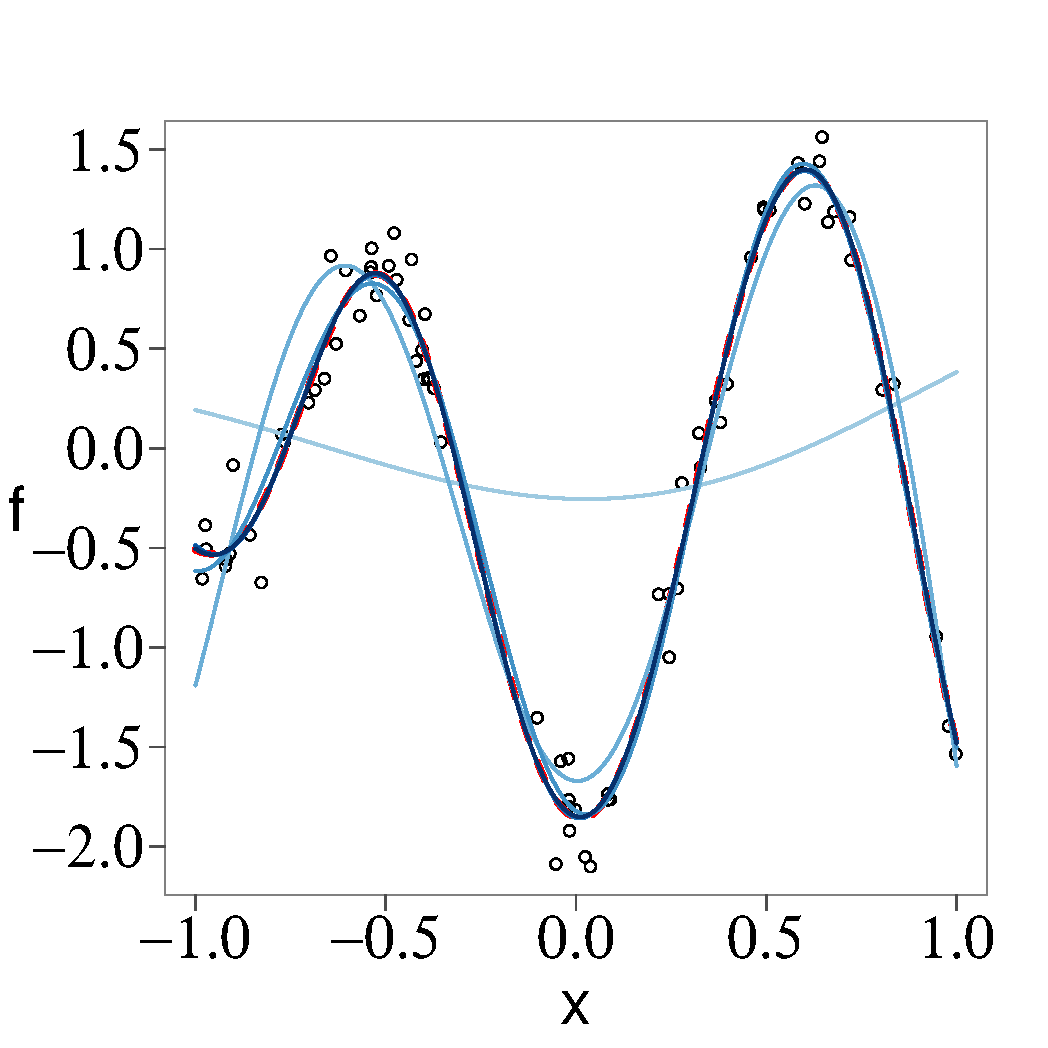
\includegraphics[scale=0.20, trim = 5mm 5mm 10mm 20mm, clip]{fig3_Post_part6.pdf} & \hspace{-5mm} 
%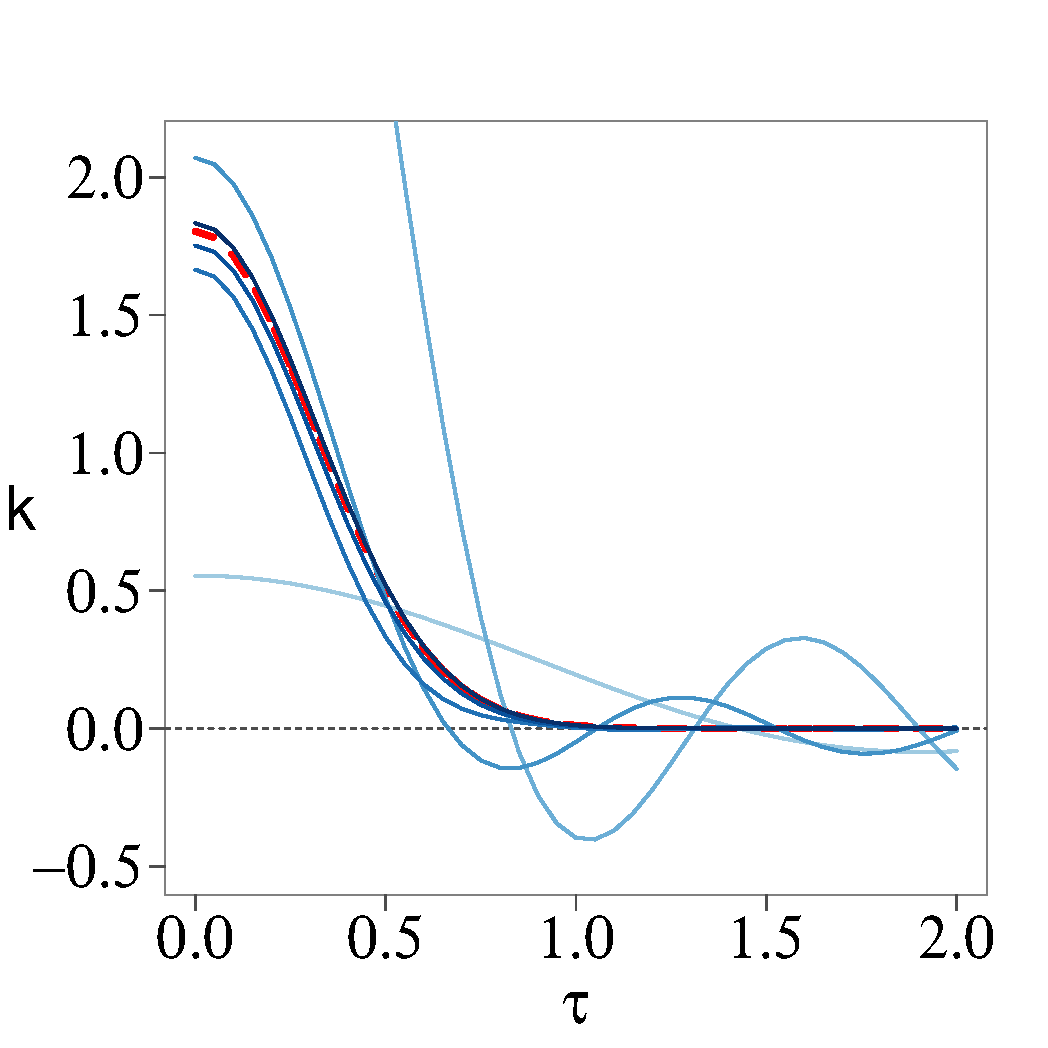
\includegraphics[scale=0.20, trim = 5mm 5mm 10mm 20mm, clip]{fig3_Cov_part6.pdf} & 
%\end{tabular}
%\caption{Mean posterior predictive functions (left-first and right-first columns) and covariance functions (left-second and right-second columns) of both the regular GP model and the HSGP model for different number of basis functions $m$ and for different values of the boundary factor $c$.}
%  \label{fig3_Post_part1}
%\end{figure}


\begin{figure}
\centering
\subfigure{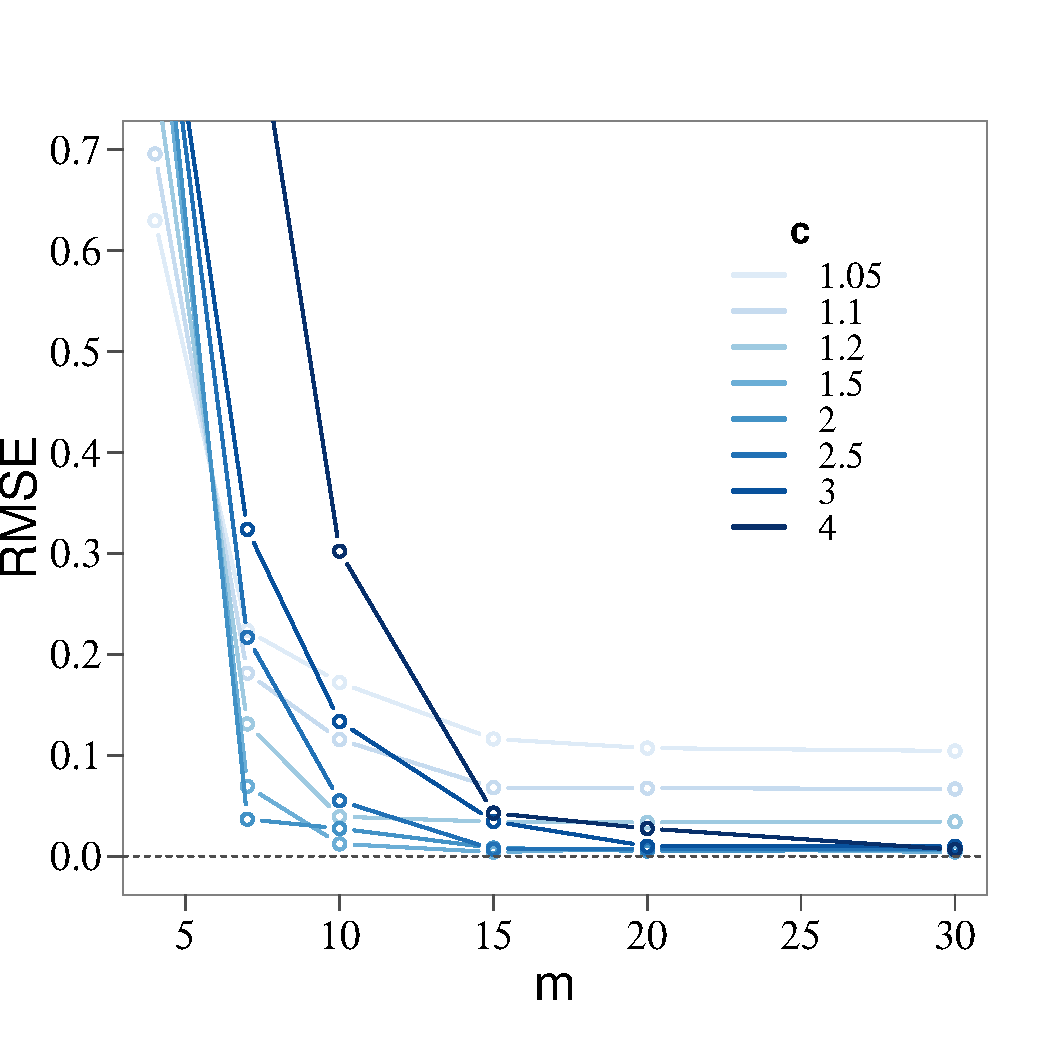
\includegraphics[scale=0.38, trim = 0mm 0mm 0mm 0mm, clip]{fig4_MSE_vs_J.pdf}}
\subfigure{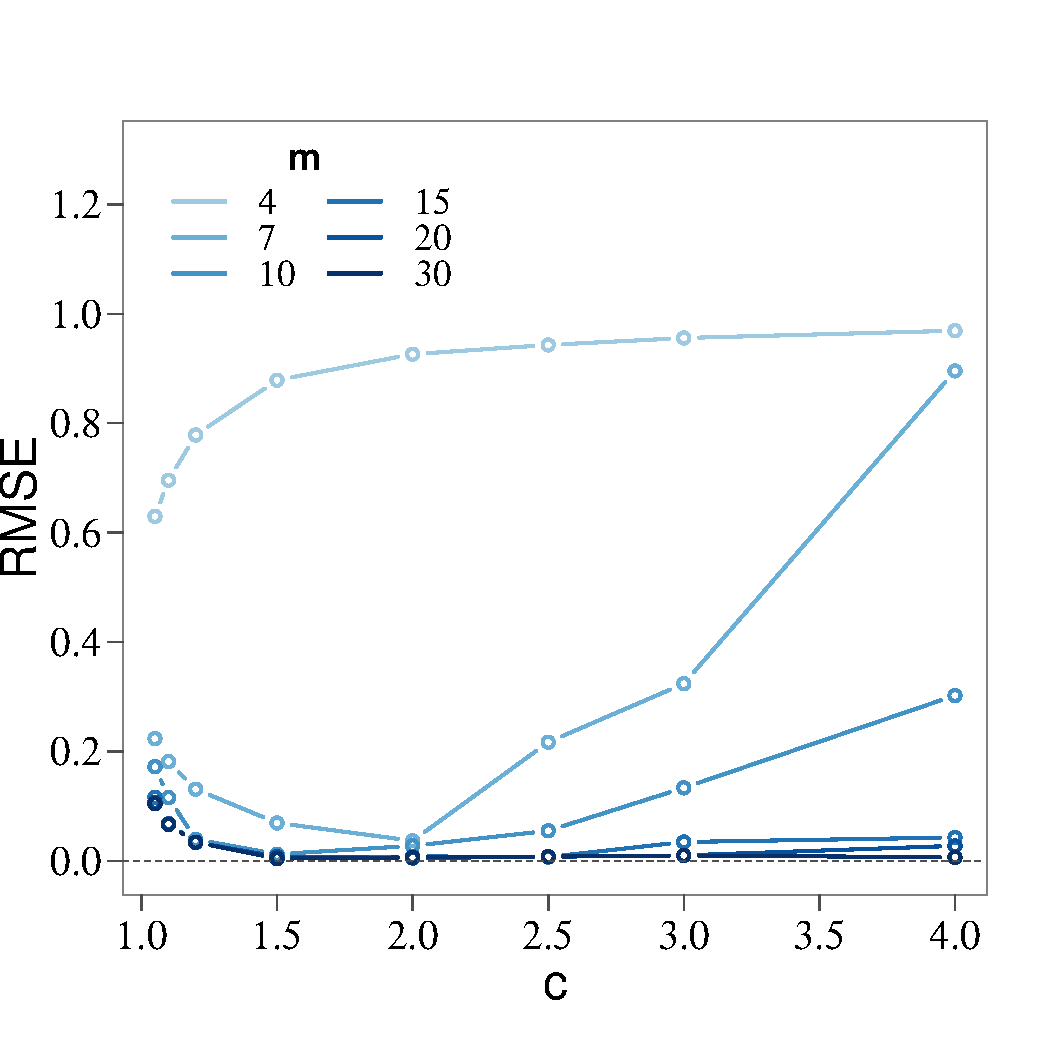
\includegraphics[scale=0.38, trim = 0mm 0mm 10mm 0mm, clip]{fig4_MSE_vs_c.pdf}}
\caption{Root mean square error (RMSE) of the proposed HSGP models computed against the regular GP model. (left) RMSE versus the number of basis functions $m$ and for different values of the boundary factor $c$. (right) RMSE versus the boundary factor $c$ and for different values of the number of basis functions $m$. }
  \label{fig4_MSE_vs_J}
\end{figure}

\begin{figure}
\centering
\subfigure{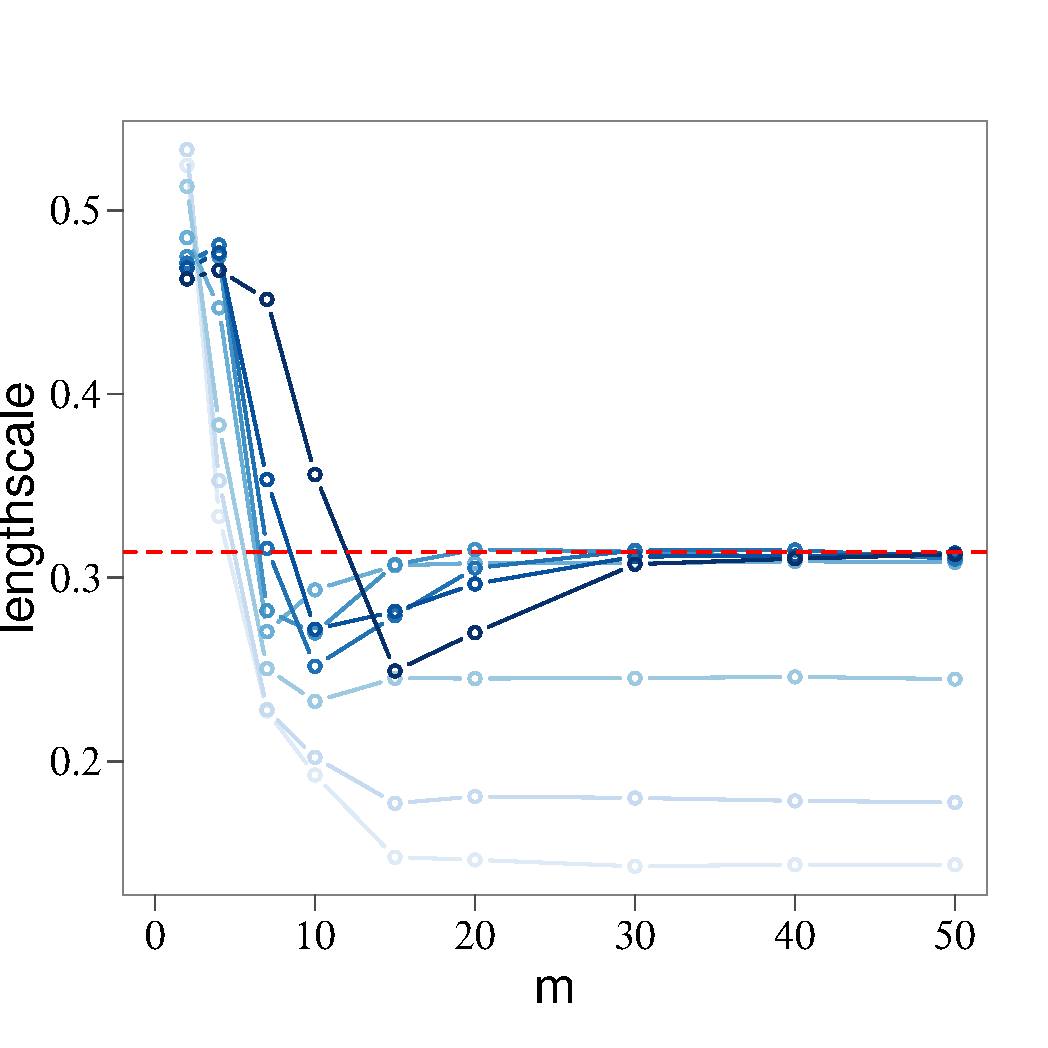
\includegraphics[scale=0.38, trim = 0mm 0mm 5mm 0mm, clip]{fig5_lscale_vs_J.pdf}}
\subfigure{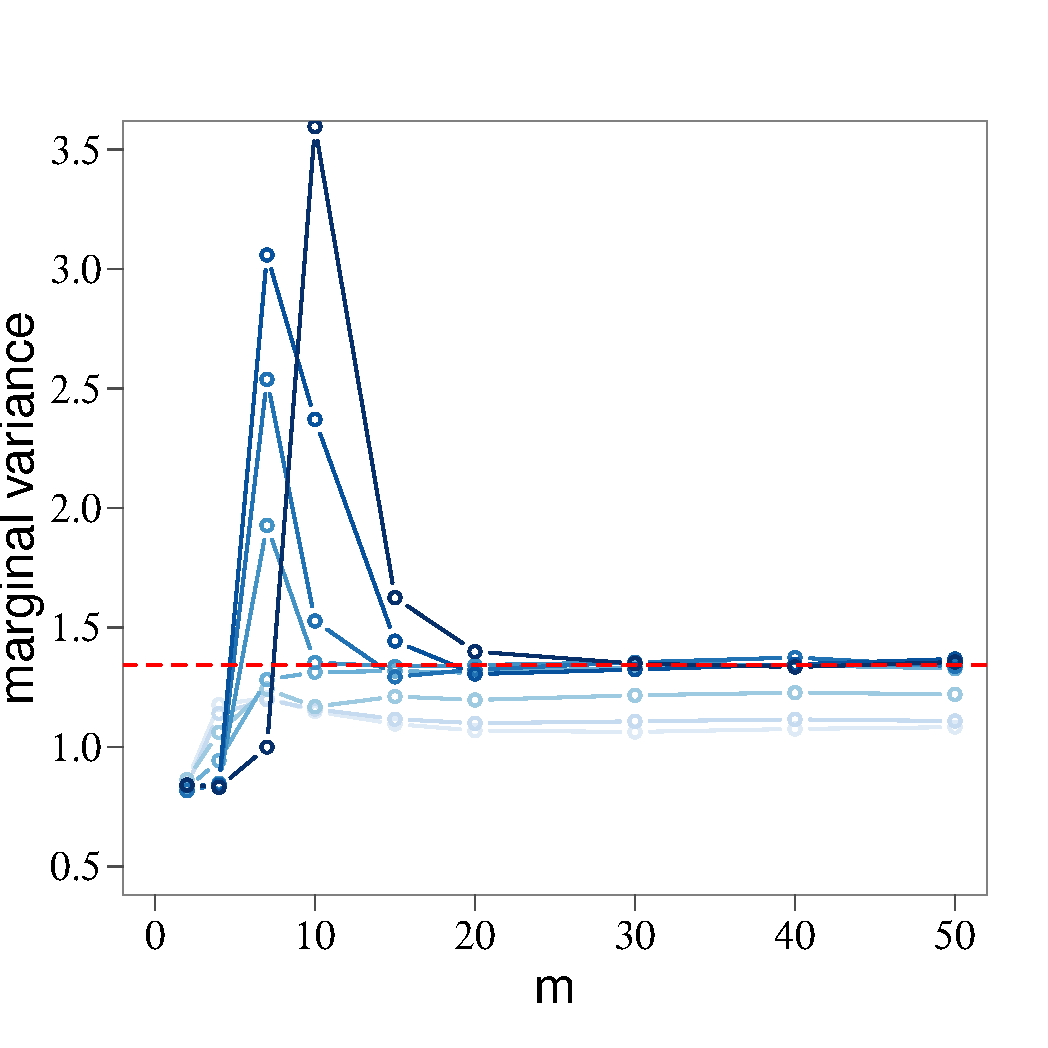
\includegraphics[scale=0.38, trim = 0mm 0mm 10mm 0mm, clip]{fig5_magnitud_vs_J.pdf}}
\subfigure{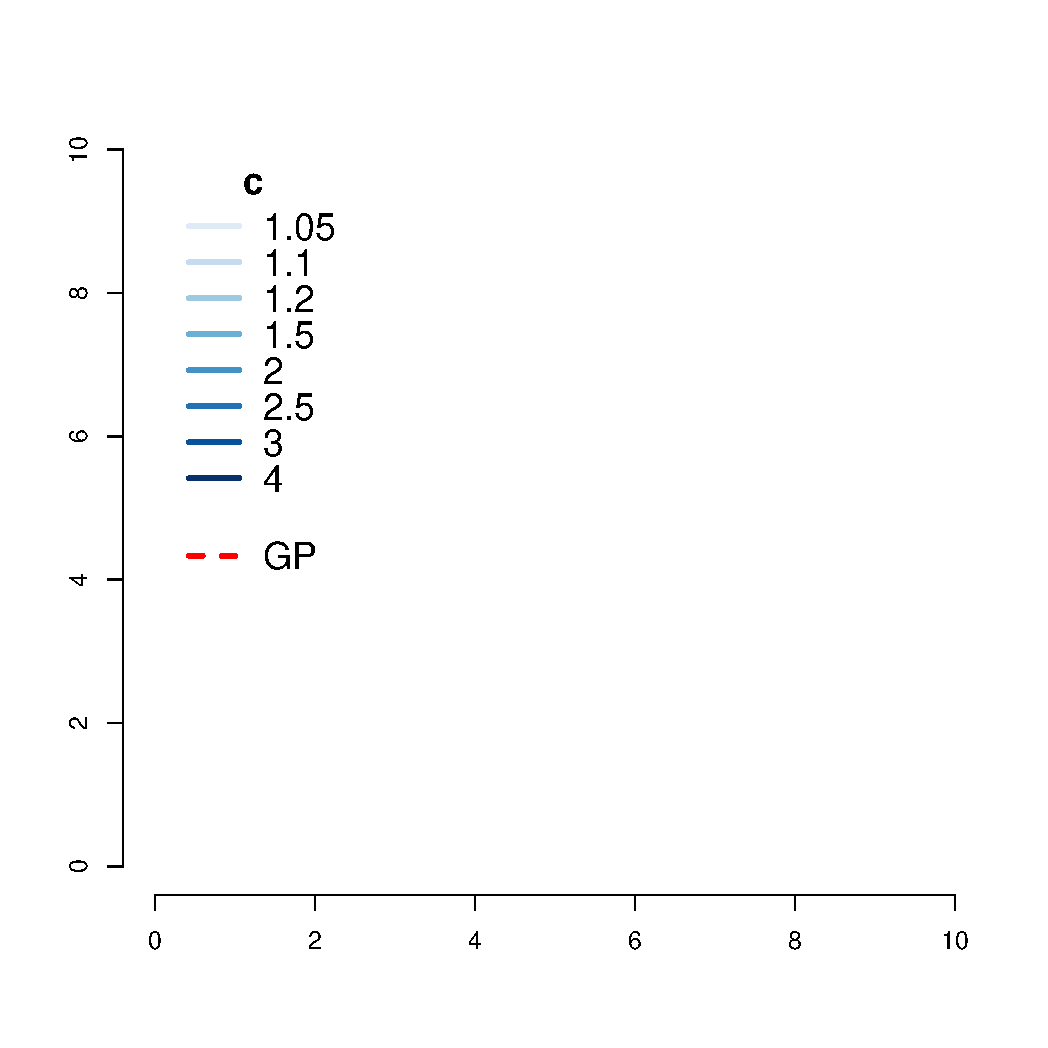
\includegraphics[scale=0.40, trim = 28mm 28mm 119mm 0mm, clip]{fig5_legend.pdf}}
\caption{Estimated lengthscale (left) and marginal variance (right) parameters of both regular GP and HSGP models, plotted versus the number of basis functions $m$ and for different values of the boundary factor $c$.}
  \label{fig5_lscale_vs_J}
\end{figure}


Additionally, there is a clear relation of the number of basis functions $m$ and the boundary factor $c$ with the lengthscale $\ell$ of the approximated function. Figures \ref{fig6_lscale_vs_J_vs_c} and \ref{fig6_lscale_vs_J_vs_c_Matern} depicts how these three factors interact with each other in relation to 
% the performance of the HSGP approximation.
a close approximation of the HSGP model, in the cases of a GP with square exponential covariance function and Mat\'ern ($\nu=3/2$) covariance function, respectively, and a single input dimension. More precisely, for a given GP model (with a square exponential covariance function) with lengthscale $\ell$ and given a boundary factor $c$, Figure \ref{fig6_lscale_vs_J_vs_c} shows the minimum $m$ required to achieve a close approximation in terms of satisfying Equation (\ref{eq_diff_covs}). Similarly for Figure \ref{fig6_lscale_vs_J_vs_c_Matern} in the case of a Mat\'ern ($\nu=3/2$) covariance function. We have considered an approximation to be a close enough when the difference between densities of the approximate covariance function and the exact covariance function, $\varepsilon$ in Equation (\ref{eq_diff_covs}), is below 1$\%$ of the density of the exact covariance function,
%
\begin{eqnarray*}
 \frac{\varepsilon}{\int k(\tau) \, d\tau} < 0.01.
\end{eqnarray*}

\noindent Alternatively, these figures could be understood as providing the minimum $c$ that we should use for given $\ell$ and $m$. Of course, we may also read it as providing the minimum $\ell$ that can be closely approximated given $m$ and $c$. We obtain the following main conclusions:

\begin{itemize}
\item As $\ell$ increases, $c$ and $m$ required for a close enough approximation decrease.
\item The lower $c$, the smaller $m$ can and $\ell$ must be to achieve a close approximation.
\item For a given $\ell$ there exist a minimum $c$ under which a close approximation is never going to be achieved regardless of $m$. This fact can be appreciated in the Figure as the contour lines which represent $c$ have an end in function of $\ell$ (Valid $c$ are restricted in function of $\ell$).
\end{itemize}

As stated above, Figures \ref{fig6_lscale_vs_J_vs_c} and \ref{fig6_lscale_vs_J_vs_c_Matern} provide the minimum lengthscale that can be closely approximated given $m$ and $c$. This information serves as a powerful diagnostic tool in determining if the obtained accuracy is acceptable. As the lenghscale $\ell$ controls the "wigglyness" of
the functional relationship, it strongly influences the difficulty of obtaining accurate
inference about the function from the data. Basically, if the lengthscale estimate is accurate, 
we can expect the HSGP approximation to be accurate as well. Thus, having obtained an estimate $\hat{\ell}$ of $\ell$ from the HSGP model based on prespecified $m$ and $c$, we can check whether or not $\hat{\ell}$ exceeds the minimum lengthscale provided in Figure \ref{fig6_lscale_vs_J_vs_c}. If $\hat{\ell}$ exceeds this recommended minimum lengthscale, the approximation should be close enough. If, however, it does not exceed it, the approximation may be inaccurate and $m$ should be increased or $c$ decreased. We may also use this diagnostic in a iterative procedure.
Starting from some initial guess of $\ell$, we can choose initial values for $m$ and $c$ and fit an HSGP model, then check the approximation accuracy, and, if not accurate enough because the estimated $\hat{\ell}$ is below the minimum lengthscale provided by Figure \ref{fig6_lscale_vs_J_vs_c}, repeat the process while increasing $m$ or decreasing $c$. Note that, as commented before, $c$ can not be decreased as much as desired because it is restricted to the lengthscale.
%replacing $\ell$ by the newly obtained estimate $\hat{\ell}$.

\begin{figure}
\centering
\subfigure{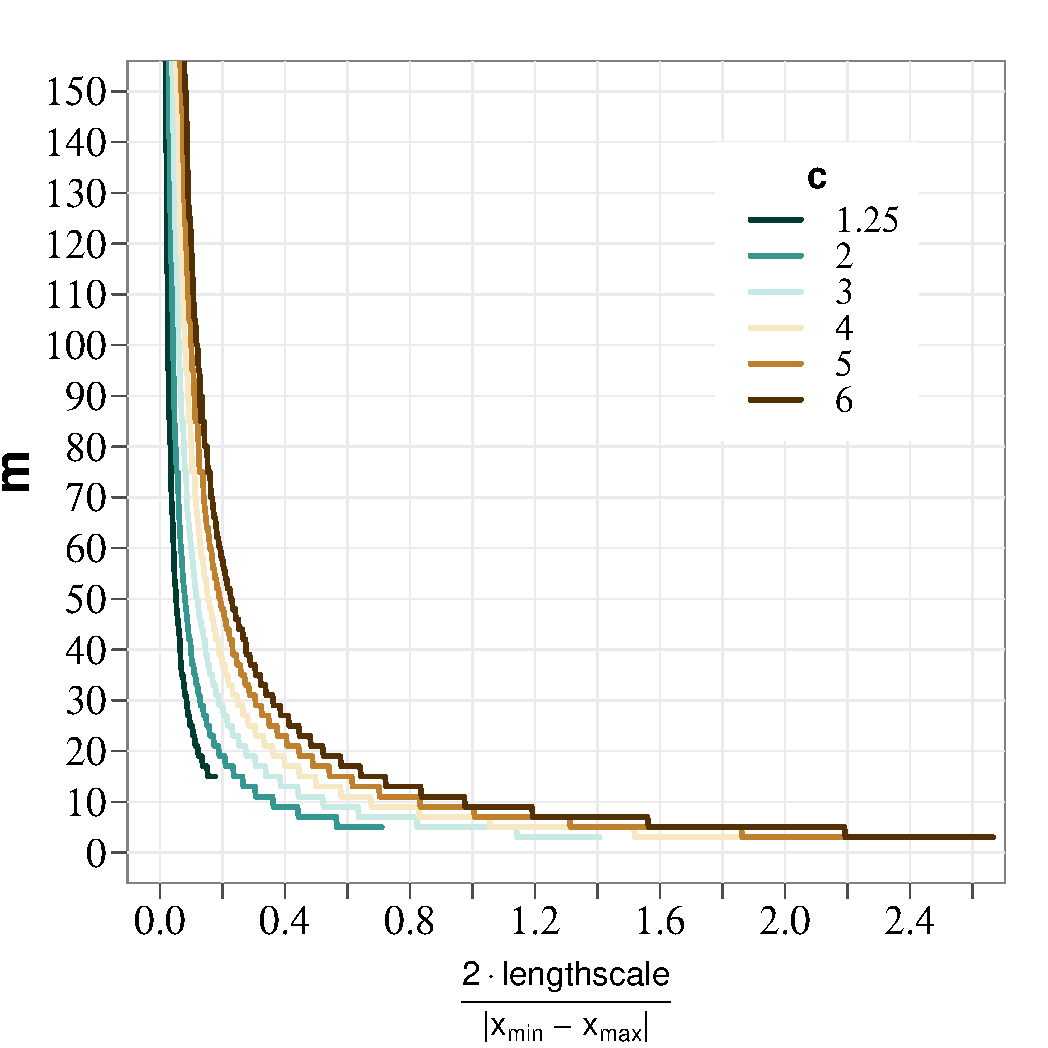
\includegraphics[scale=0.40, trim = 0mm 0mm 5mm 0mm, clip]{fig6_lscale_vs_J_vs_c.pdf}}
\hspace{3mm}
\subfigure{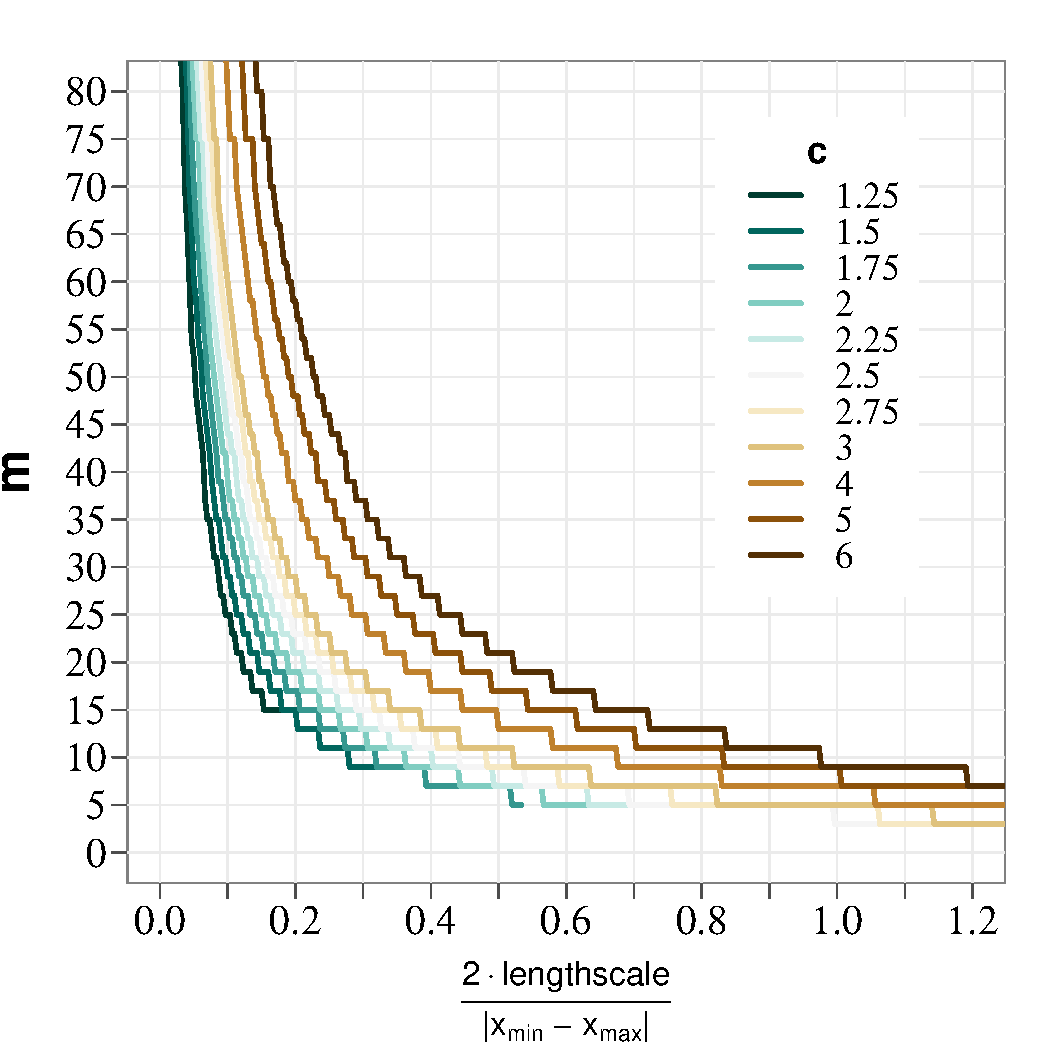
\includegraphics[scale=0.40, trim = 0mm 0mm 5mm 0mm, clip]{fig6_lscale_vs_J_vs_c_zoomin.pdf}}
\caption{Relation among the minimum number of basis functions $m$, the boundary factor $c$ ($c = \frac{L}{S}$) and the lengthscale normalized by the half-range of the data ($\frac{\ell}{S}$), in the case of a square exponential covariance function. The right-side plot is a zoom in of the left-side plot.}
  \label{fig6_lscale_vs_J_vs_c}
\end{figure}

\begin{figure}
\centering
\subfigure{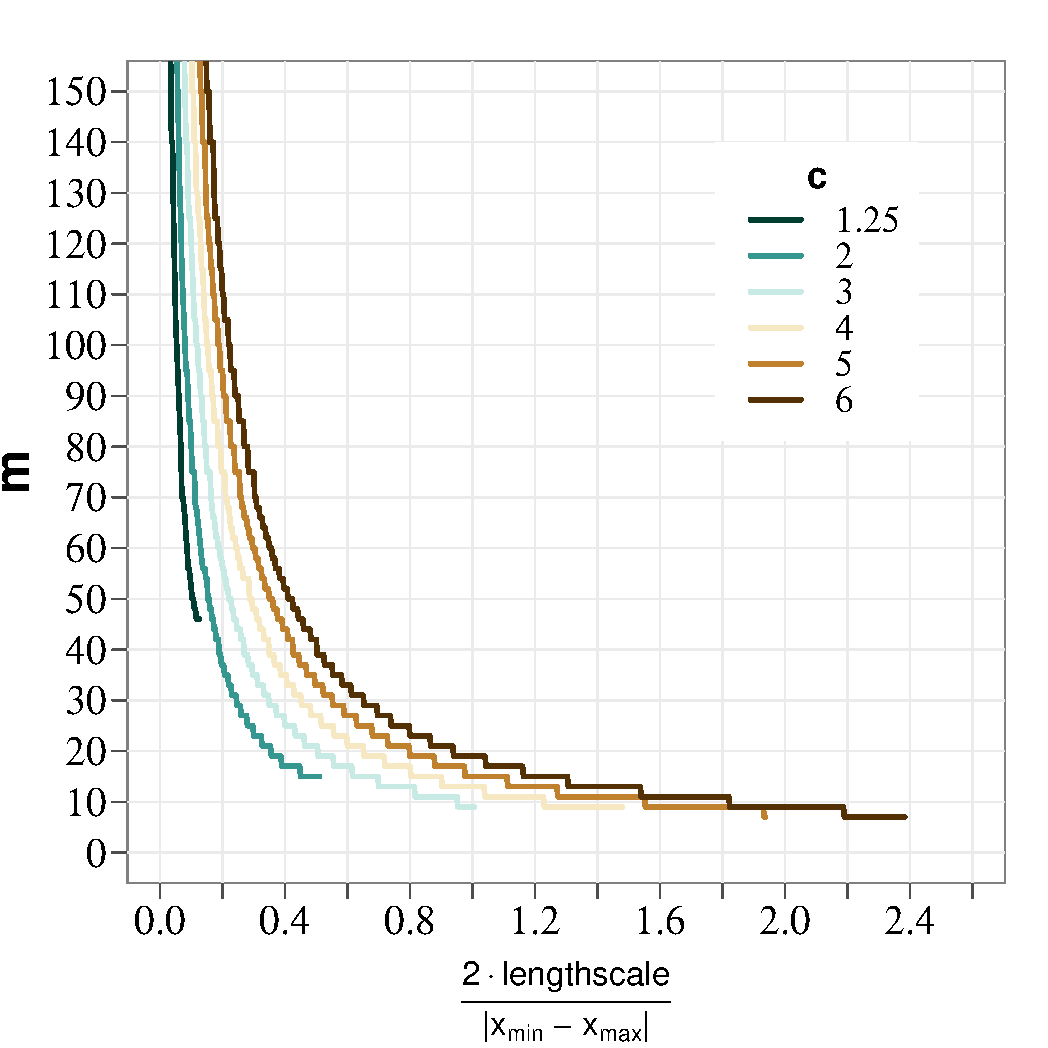
\includegraphics[scale=0.40, trim = 0mm 0mm 5mm 0mm, clip]{fig6_lscale_vs_J_vs_c_Matern.pdf}}
\hspace{3mm}
\subfigure{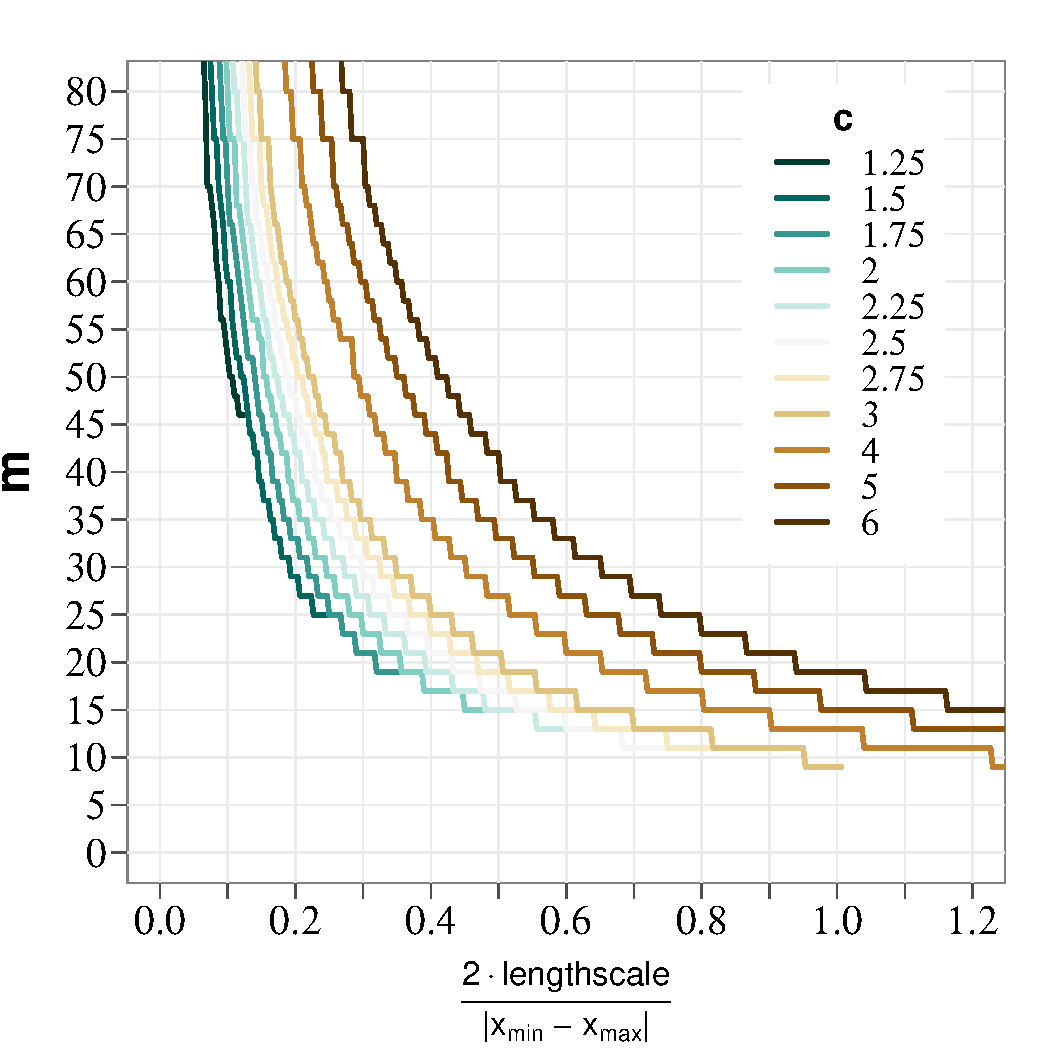
\includegraphics[scale=0.40, trim = 0mm 0mm 5mm 0mm, clip]{fig6_lscale_vs_J_vs_c_zoomin_Matern.pdf}}
\caption{Relation among the minimum number of basis functions $m$, the boundary factor $c$ ($c = \frac{L}{S}$) and the lengthscale normalized by the half-range of the data ($\frac{\ell}{S}$), in the case of a Mat\`ern($\frac{3}{2}$) covariance function. The right-side plot is a zoom in of the left-side plot.}
  \label{fig6_lscale_vs_J_vs_c_Matern}
\end{figure}


If we look back to the conclusions drawn from Figures \ref{fig4_MSE_vs_J} and \ref{fig5_lscale_vs_J}, where $m = 10$ basis functions and a boundary factor of $c = 1.5$ were enough to closely approximate a function with $\ell = 0.3$, we can recognize that these conclusions also matches those obtained from Figure \ref{fig6_lscale_vs_J_vs_c}.

Figures \ref{fig6_lscale_vs_J_vs_c} and \ref{fig6_lscale_vs_J_vs_c_Matern} were build for a GP with a unidimensional covariance function, which result in a surface depending on three variables, $m$, $c$ and $\ell$. An equivalent figure for a GP model with a two-dimensional covariance function would result in a surface depending on four variables, $m$, $c$, $\ell_1$ and $\ell_2$, which can not be graphically represented. However, as an approximation we can use the unidimensional GP conclusions in Figures \ref{fig6_lscale_vs_J_vs_c} and \ref{fig6_lscale_vs_J_vs_c_Matern} to analyze individually the different dimensions of a multidimensional GP model. 

(Gabi: Perhaps, in the two-dimensional case, whether the approximation is close enough might depend only on the ratio between the variables $\ell_1$ and $\ell_2$.)

\subsection{Comparing lengthscale estimates}

In this example, we make a comparison of the lengthscale estimates
obtained from the regular GP and HSGP models. We also have a look at those recommended minimum lengthscales provided by Figure \ref{fig6_lscale_vs_J_vs_c}.

%Another way to look at the approximation accuracy of HSGPs is to compare the lengthscale estimates
%obtained from the regular GP and HSGP models. As the lenghscale $\ell$ controls the "wigglyness" of
%the functional relationship, it strongly influences the difficulty of obtaining accurate
%inference about the function from the data. Basically, if the lengthscale estimate is accurate, 
%we can expect the HSGP approximation to be accurate as well.

For this analysis, we will use various datasets consisting of noisy draws from a GP prior model with a squared exponential covariance function and varying lengthscale values. Different values of the number of basis functions $m$ are used when estimating the HSGP models, and the boundary factor $c$ is set to a valid and optimum value in every case. 

Figure \ref{fig7_posterior_varing_lscale_part1} shows the posterior predictions of both regular GP and HSGP models fitted to those datasets. The lengthscale estimates as obtained by regular GP and HSGP models are depicted in Figure \ref{fig8_Tlscale_vs_Elscale}. As noted previously, an accurate estimate of the lengthscale can be a good indicator of a close approximation of the HSGP model to the regular GP model. Further, Figure \ref{fig9_MSE_varing_lscale} shows the root mean square error (RMSE) of the HSGP models, computed against the regular GP models, as a function of the lengthscale and number of basis functions.

\begin{figure}
\centering
\subfigure{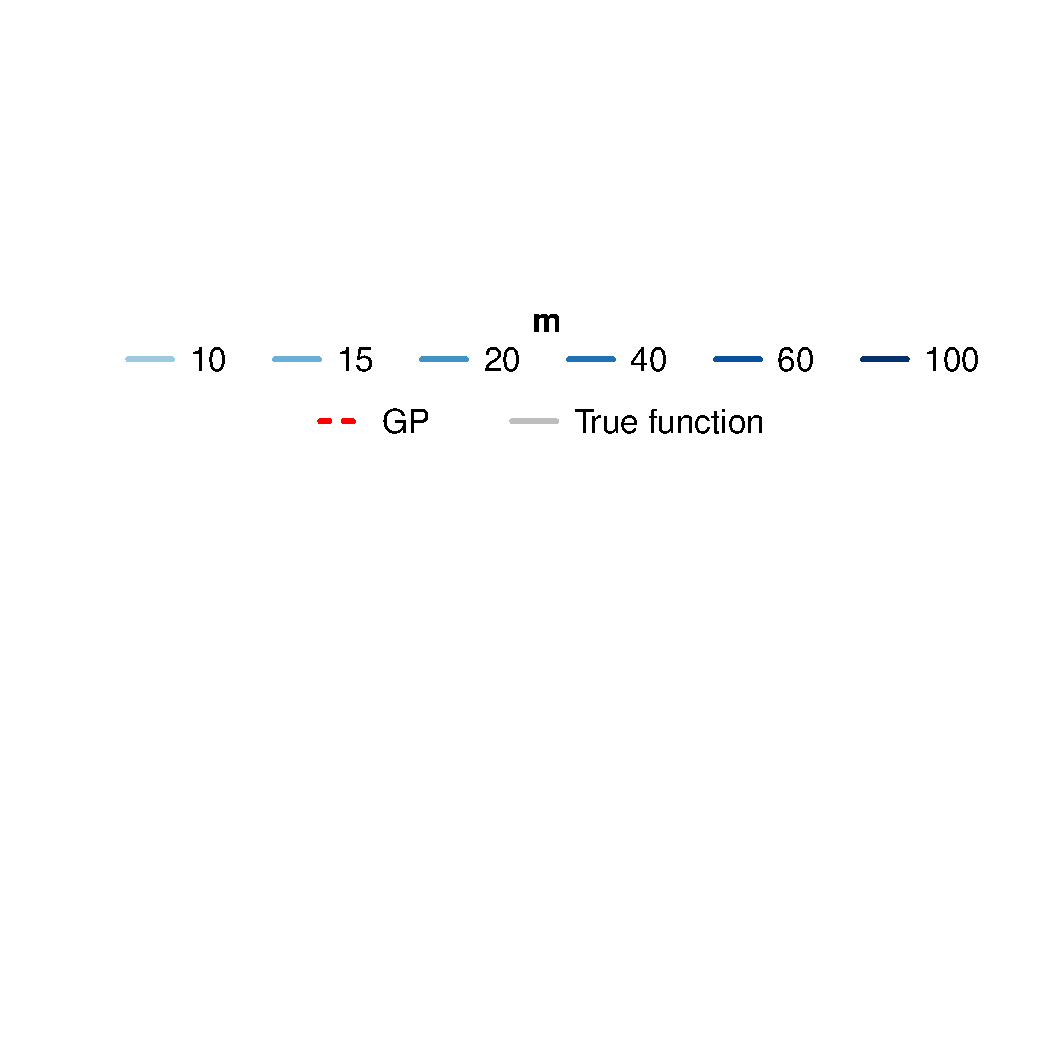
\includegraphics[scale=0.4, trim = 10mm 100mm 5mm 30mm, clip]{fig7_legend.pdf}}\\
\vspace{-3mm}
\subfigure{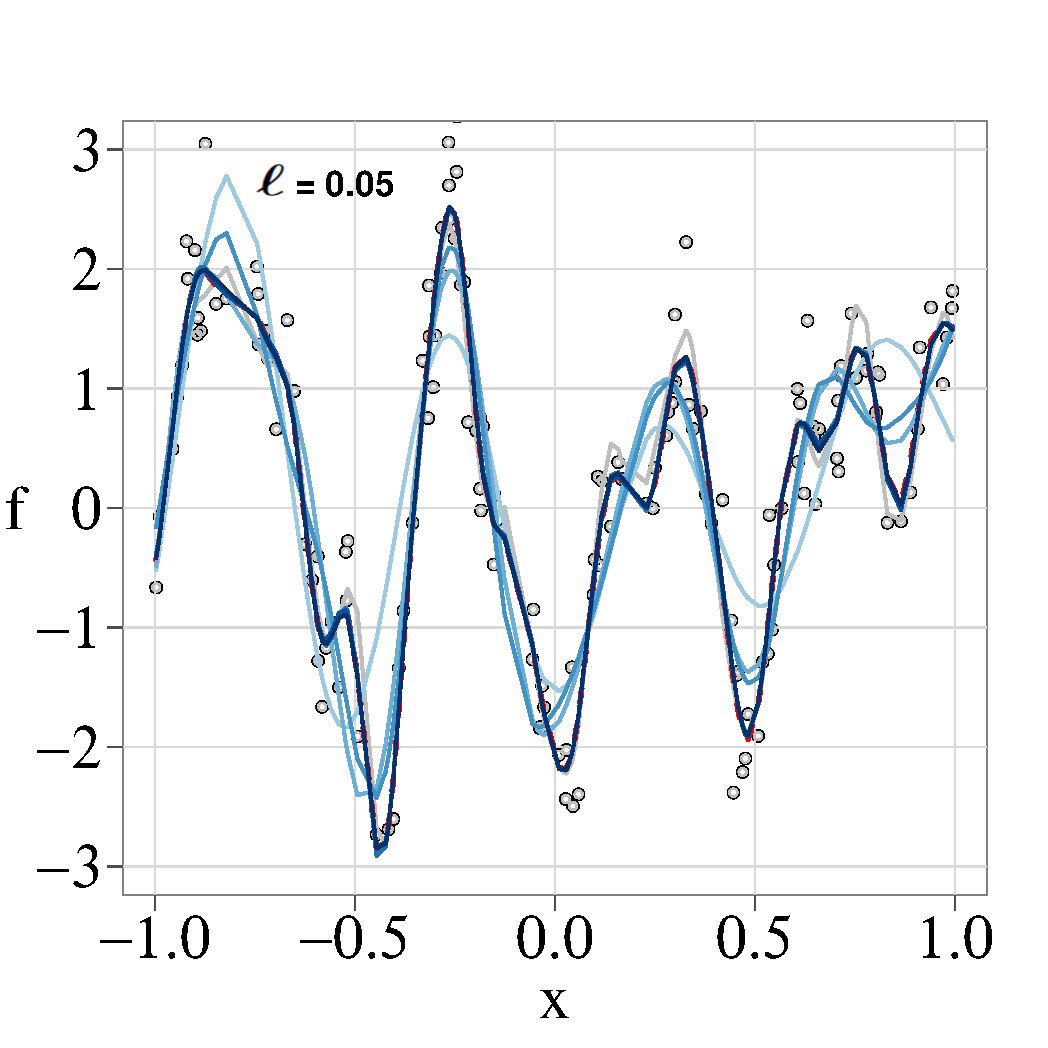
\includegraphics[scale=0.30, trim = 1mm 25.5mm 10mm 19mm, clip]{fig7_posterior_varing_lscale_part1.pdf}}
\subfigure{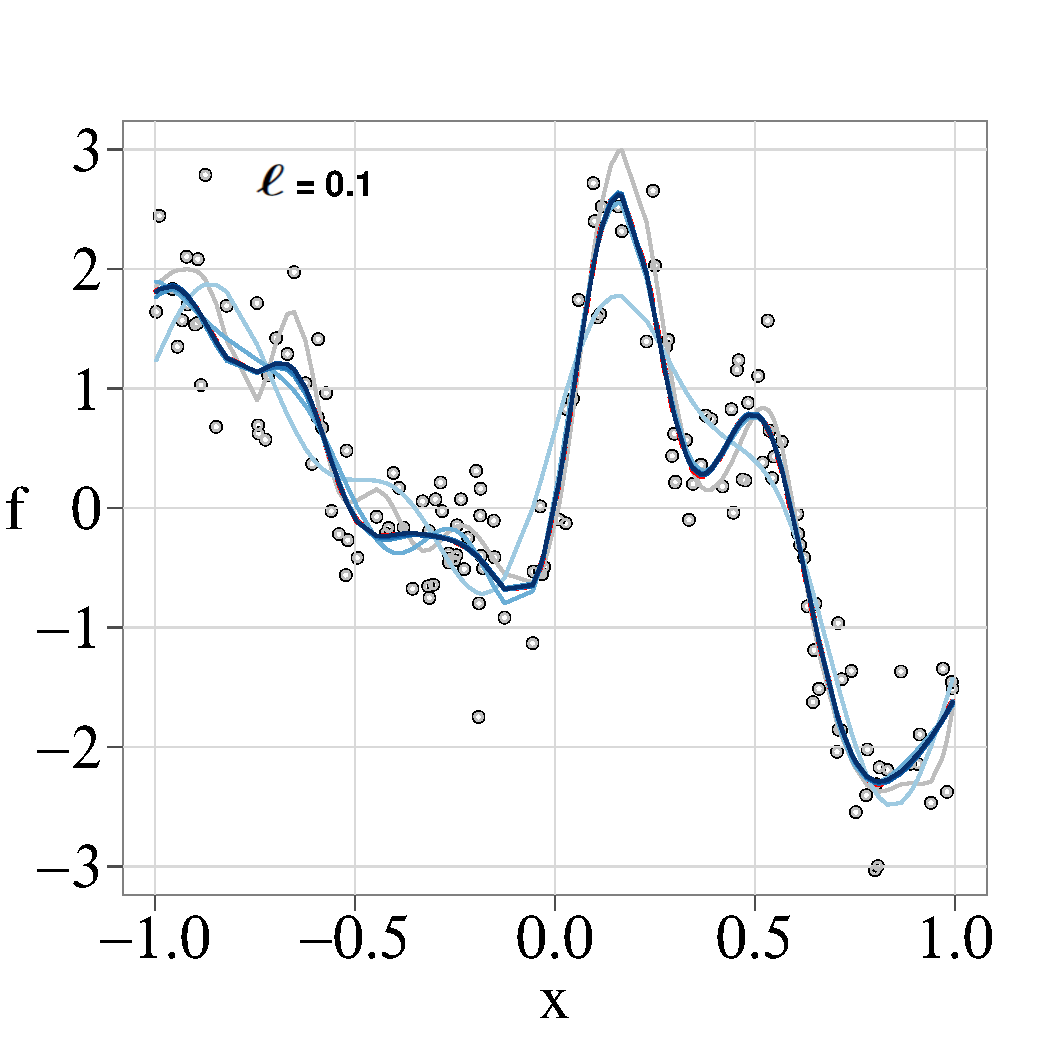
\includegraphics[scale=0.30, trim = 21mm 25.5mm 10mm 19mm, clip]{fig7_posterior_varing_lscale_part2.pdf}}
\subfigure{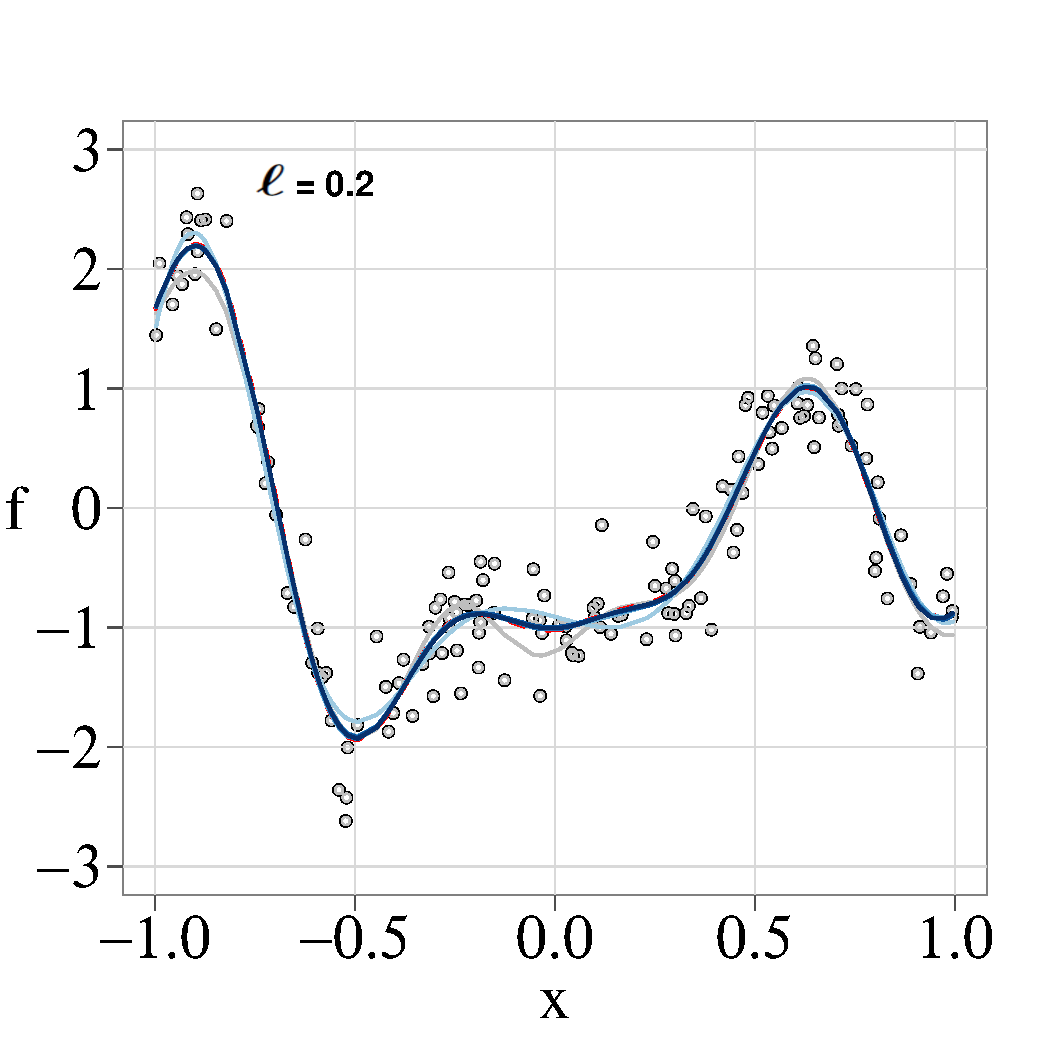
\includegraphics[scale=0.30, trim = 21mm 25.5mm 10mm 19mm, clip]{fig7_posterior_varing_lscale_part3.pdf}}\\
\vspace{-3mm}
\subfigure{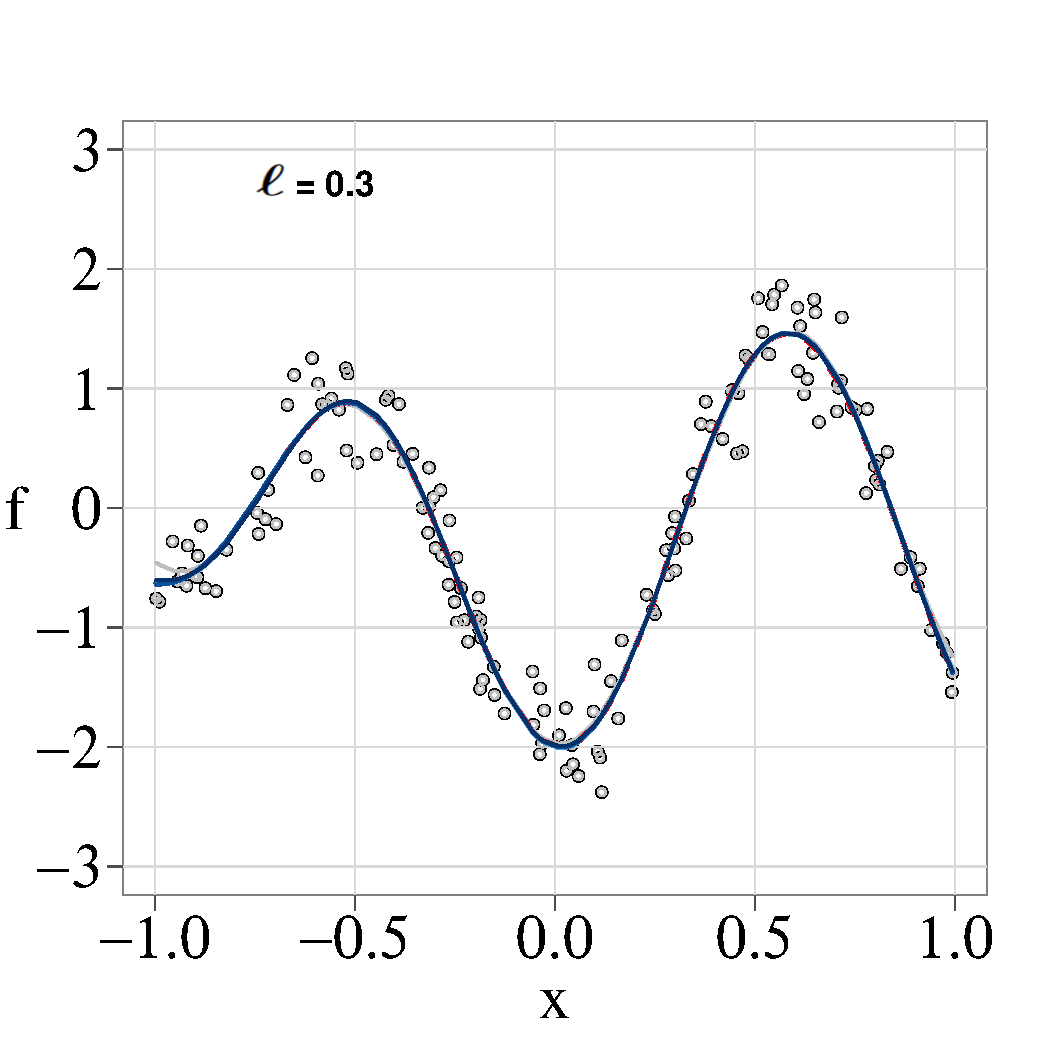
\includegraphics[scale=0.30, trim = 1mm 25.5mm 10mm 19mm, clip]{fig7_posterior_varing_lscale_part4.pdf}}
\subfigure{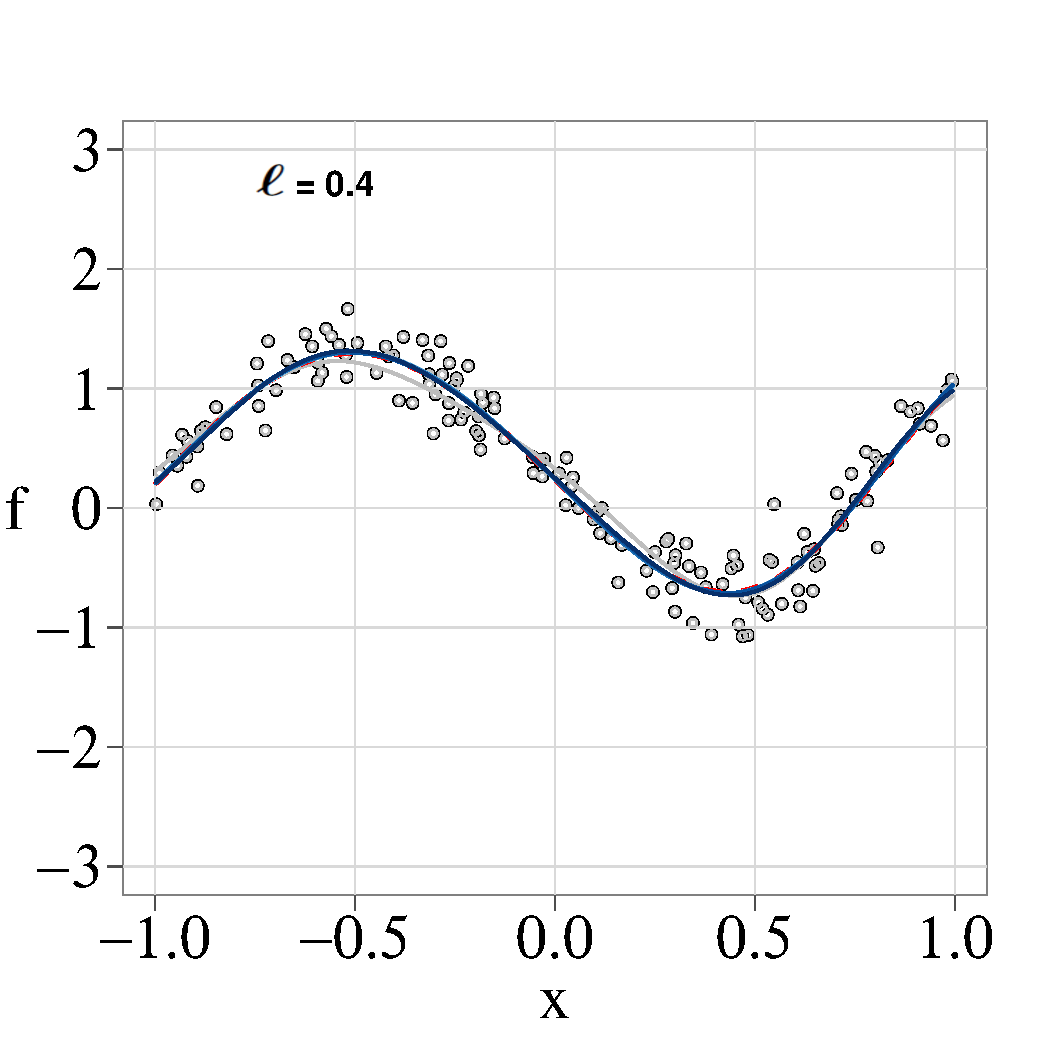
\includegraphics[scale=0.30, trim = 21mm 25.5mm 10mm 19mm, clip]{fig7_posterior_varing_lscale_part5.pdf}}
\subfigure{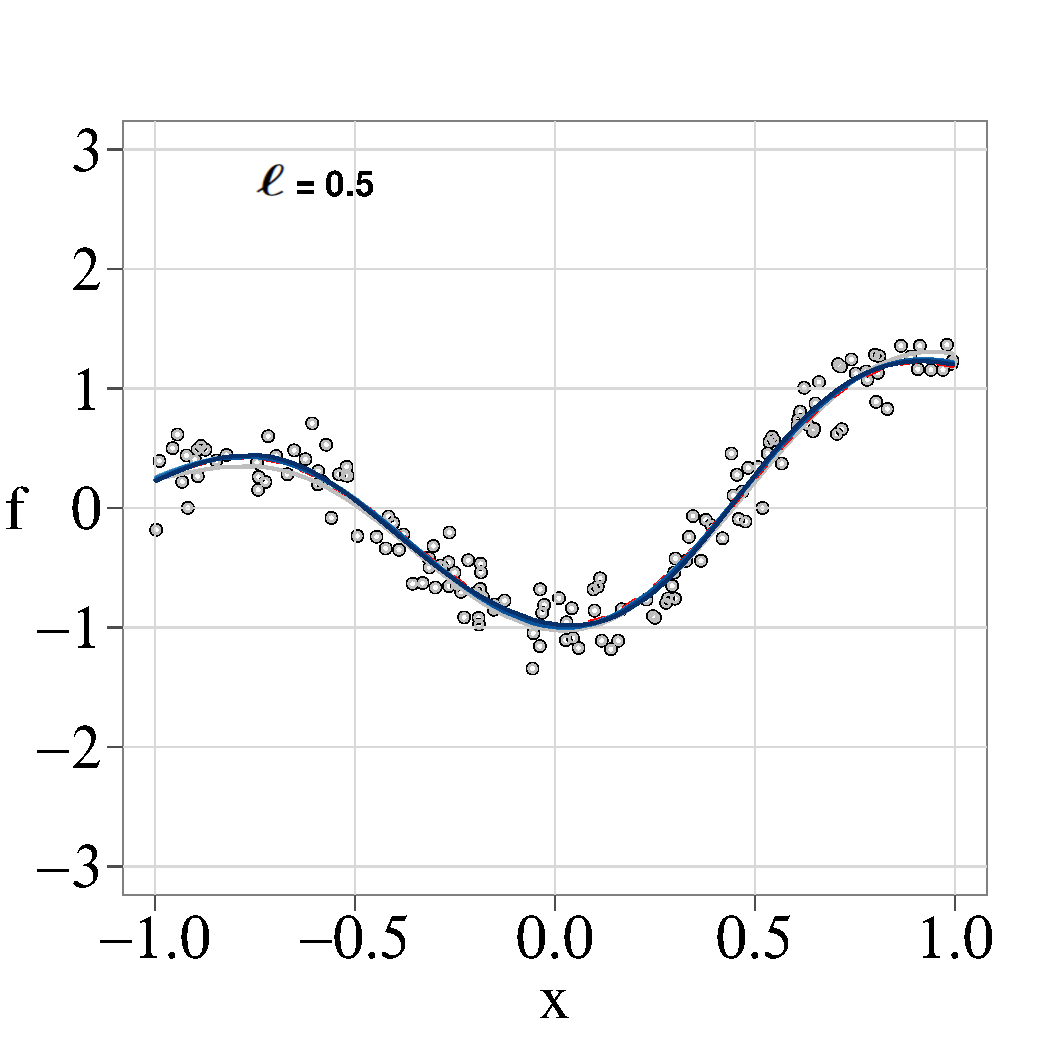
\includegraphics[scale=0.30, trim = 21mm 25.5mm 10mm 19mm, clip]{fig7_posterior_varing_lscale_part6.pdf}}\\
\vspace{-3mm}
\subfigure{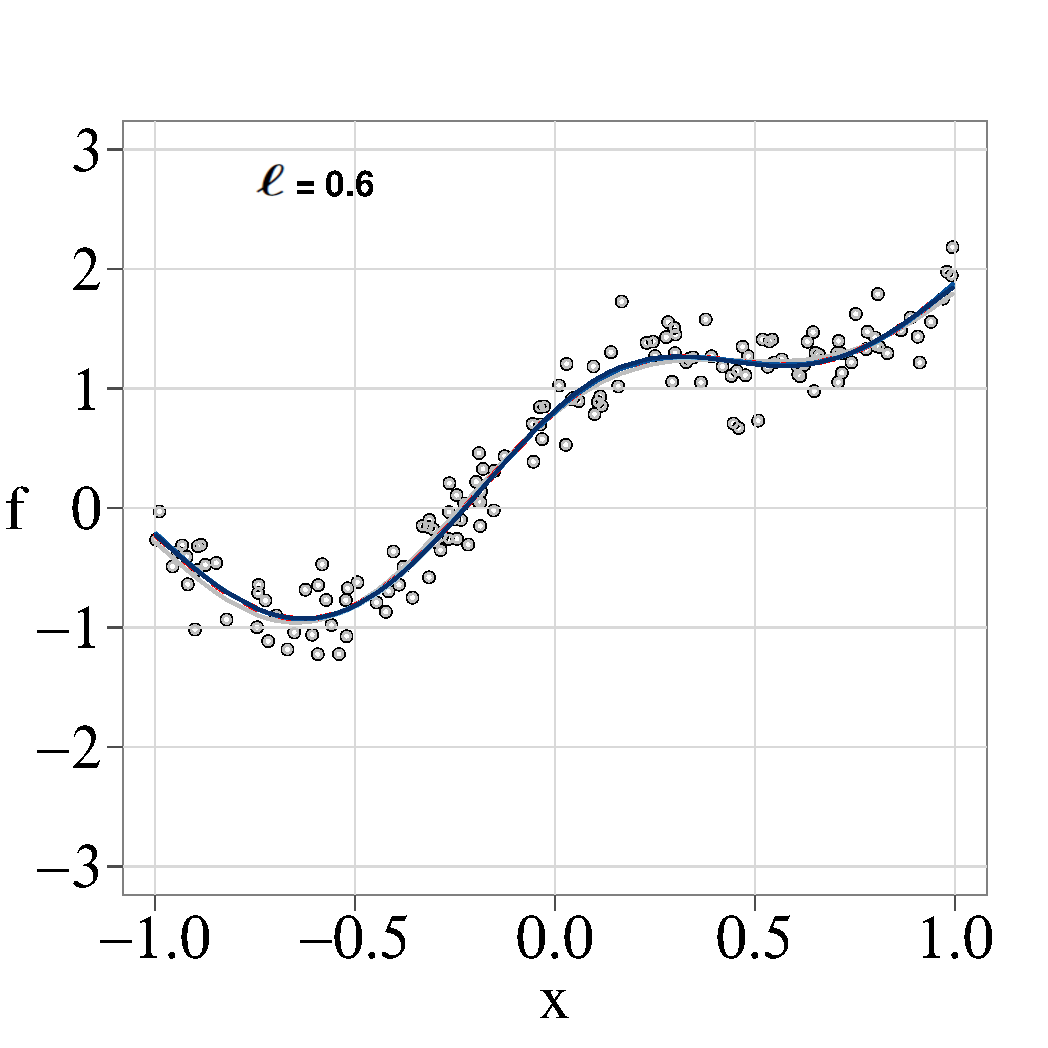
\includegraphics[scale=0.30, trim = 1mm 5mm 10mm 19mm, clip]{fig7_posterior_varing_lscale_part7.pdf}}
\subfigure{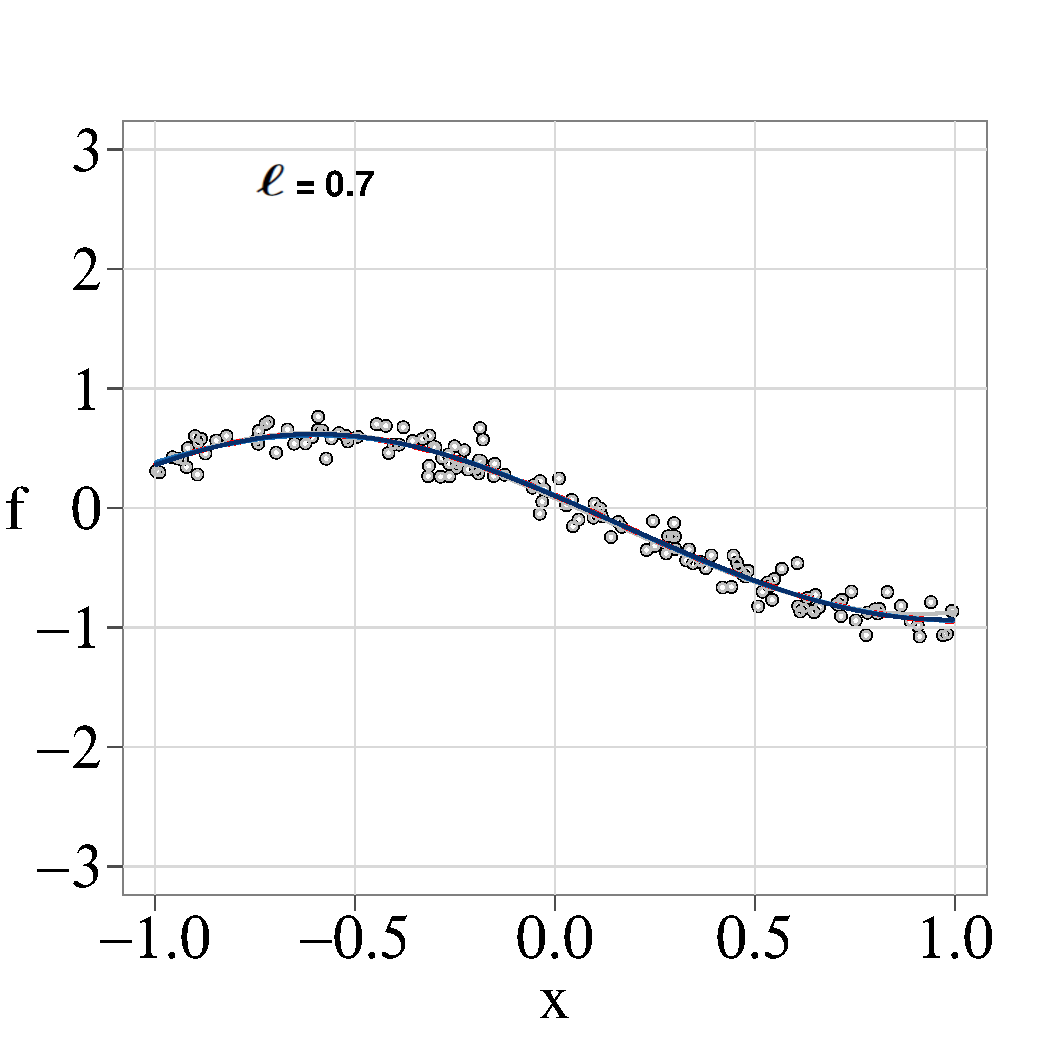
\includegraphics[scale=0.30, trim = 21mm 5mm 10mm 19mm, clip]{fig7_posterior_varing_lscale_part8.pdf}}
\subfigure{\includegraphics[scale=0.30, trim = 21mm 5mm 10mm 19mm, clip]{fig7_posterior_varing_lscale_part9.pdf}}\\
\vspace{-3mm}
\caption{Mean posterior predictions of both regular GP and HSGP models, fitted over various datasets drawn from square exponential GP models with different characteristic lengthscales ($\ell$) and same marginal variance ($\alpha$) as the data-generating functions (\textit{True function}).}
  \label{fig7_posterior_varing_lscale_part1}
\end{figure}

\begin{figure}
\begin{flushleft}
\begin{tabular}{ccc}
\multicolumn{3}{c}{ \includegraphics[scale=0.40, trim = 25mm 117mm 90mm 45mm, clip]{fig8_legend.pdf}}\\
\includegraphics[scale=0.30, trim = 0mm 24mm 7mm 10mm, clip]{fig8_Tlscale_vs_Elscale_part1.pdf} & \hspace{-4mm}
\includegraphics[scale=0.30, trim = 25mm 24mm 7mm 10mm, clip]{fig8_Tlscale_vs_Elscale_part2.pdf} & \hspace{-4mm} \includegraphics[scale=0.30, trim = 25mm 24mm 7mm 10mm, clip]{fig8_Tlscale_vs_Elscale_part3.pdf} \\ 
\includegraphics[scale=0.30, trim = 0mm 0mm 7mm 10mm, clip]{fig8_Tlscale_vs_Elscale_part4.pdf} & \hspace{-4mm} \includegraphics[scale=0.30, trim = 25mm 0mm 7mm 10mm, clip]{fig8_Tlscale_vs_Elscale_part5.pdf} & \hspace{-4mm} \includegraphics[scale=0.30, trim = 25mm 0mm 7mm 10mm, clip]{fig8_Tlscale_vs_Elscale_part6.pdf}
\end{tabular}
\end{flushleft}
\caption{Data-generating functional lengthscales ($\ell$), of the various datasets illustrated in Figure \ref{fig7_posterior_varing_lscale_part1}, versus the corresponding lengthscale estimates $(\hat{\ell})$ from the regular GP and HSGP models. 95\% confident intervals of the lengthscale estimates are plotted as dot lines. The different plots represent the use of different number of basis functions $m$ in the HSGP model. The dashed black line represents the recommended minimum lengthscales provided by Figure \ref{fig6_lscale_vs_J_vs_c} that can be closely approximated by the HSGP model in every case.}
  \label{fig8_Tlscale_vs_Elscale}
\end{figure}


\begin{figure}
\centering
\includegraphics[scale=0.38]{fig9_MSE_varing_lscale.pdf}
\caption{RMSE of the HSGP models with different number of basis functions $m$, for the various datasets with different wiggly effects ($\ell$).}
  \label{fig9_MSE_varing_lscale}
\end{figure}

Comparing the accuracy of the lengthscale in Figure 
\ref{fig8_Tlscale_vs_Elscale} to the RMSE in Figure \ref{fig9_MSE_varing_lscale},
we see that they agree closely with each other for medium lengthscales.
That is, a good estimation of the lengthscale implies a
small RMSE. This is no longer true for very small or large lengthscales.
In small lengthscales, even very small inaccuracies 
may have a strong influence on the posteriors predictions and thus on the RMSE.
In large lengthscales, larger inaccuracies change the posterior predictions
only little and may thus not yield large RMSEs.
The dashed black line in Figure \ref{fig8_Tlscale_vs_Elscale} represents the 
minimum lengthscale that can be closely approximated under the given condition, according to the results presented in Figure \ref{fig6_lscale_vs_J_vs_c}. 
We observe that whenever the estimated lengthscale exceeds the minimially
estimable lengthscale, the RMSE of the posterior predictions is small
(see Figure \ref{fig9_MSE_varing_lscale}).
Conversely, when the estimated lengthscale is smaller than the minimally
estimable one, the RMSE becomes very large.

(Paul: Figure 8 and 9 are not rendered correctly in my PDF viewer after 
compiling the tex file, which has something to do with the font of the facet 
and legend labels I believe. Latex also issues warnings about this.)

% Comparing the information of models approximation provided by Figures \ref{fig8_Tlscale_vs_Elscale} and \ref{fig9_MSE_varing_lscale}, it can be appreciated an agreement between both figures, excepting for small lengthscales and long lengthscales. We observe small RMSE for large lengthscales in Figure \ref{fig9_MSE_varing_lscale}, however there exist mismatch between large lengthscale estimates of GP and HSGP models in Figure \ref{fig8_Tlscale_vs_Elscale}. This is because big changes on large lengthscales, which might be clearly appreciated in Figure \ref{fig8_Tlscale_vs_Elscale}, might result in similar posterior predictions and therefore a small RMSE. On the other side, we observe high RMSE for small lengthscales in Figure \ref{fig9_MSE_varing_lscale}, however there exist match between small lengthscale estimates of GP and HSGP models in Figure \ref{fig8_Tlscale_vs_Elscale}. This is because very small changes on small lengthscales, which might not be appreciated in Figure \ref{fig8_Tlscale_vs_Elscale}, can have big effects on the posteriors predictions and therefore high RMSE.

%The dashed black line in Figure \ref{fig8_Tlscale_vs_Elscale} represents the minimum lengthscales that can be closely approximate in every case, according to Figure \ref{fig6_lscale_vs_J_vs_c}. It can be appreciated a complete agreement between those recommended minimum lengthscales that can be properly fitted in every case following Figure \ref{fig6_lscale_vs_J_vs_c} and the real approximate accuracy measured by the RMSE in Figure \ref{fig9_MSE_varing_lscale}.


\section{Univariate examples}


\subsection{Study case I: Simulated data}

This example consists of a simulated dataset with 250 ($i=1,\dots,n=250$) single draws from a Gaussian process prior with a Mat{\'e}rn($\nu$=3/2) covariance function and hyperparameters marginal variance $\alpha=1$ and lengthscale $\ell=0.15$, with corresponding inputs values $\bm{x}=\{x_i\}_{i=1}^{250}$ with $x_i \in [-1,1] \subset {\rm I\!R}$. To form the final noisy dataset $\bm{y}$, Gaussian noise $\sigma=0.2$ was added to the GP draws.

The regular GP model for fitting this simulated dataset $\bm{y}$ can be written as follows,
%
\begin{eqnarray*}\label{eq_latentgp_simudata1}
\begin{split}
\bm{y} &= f(\bm{x}) + \bm{\epsilon} \\
\bm{\epsilon} &\sim \mathcal{N}(0, \sigma^2  I) \\
f(\bm{x}) &\sim \mathcal{GP}(0, k(\bm{x}, \bm{x}', \theta)),
\end{split}
\end{eqnarray*}

\noindent where $I$ represents the identity matrix. The previous formulation corresponds to the latent form of a GP model, where $f(\bm{x})$ represents the underlying functional model to the noisy data and is modeled by a GP prior with a Mat{\'e}rn($\nu=3/2$) covariance function $k$. Saying that the function values $f(\bm{x})$ follows a GP model is equivalent to say that $f(\bm{x})$ are multivariate Gaussian distributed with covariance matrix $K$, where $K_{ij}=k(x_i,x_j,\theta)$.
 
A more computationally efficient formulation of a GP model with Gaussian likelihood, and for probabilistic inference using sampling methods such as HMC, would be its marginalized form,
%
\begin{equation*}\label{eq_marginalizedgp_simudata1}
\bm{y} \sim \mathcal{N}(0, K + \sigma^2 I ),
\end{equation*}

\noindent where the function values $f(\bm{x})$ have been integrated out, yielding a lower-dimensional parameter space over which to do inference, reducing time of computation and improving the sampling and the effective number of samples.

In the HSGP model, the latent function values $f(\bm{x})$ are approximated as (\ref{eq_approxf}),
%
\begin{equation*}
f(\bm{x}) \approx \sum_{j}^m \left( S(\sqrt{\lambda_j})\right)^{1/2} \phi_j(\bm{x}) \beta_j,
\end{equation*}

\noindent with the spectral density $S$ (\ref{eq_specdens_32}) as a function of $\sqrt{\lambda_j}$,
%
\begin{eqnarray*}
S(\sqrt{\lambda_j})&=& \alpha^2 \frac{4\sqrt{3}^{3}}{\ell^3}(\frac{3}{\ell^2} + \lambda_j)^{-2}, 
\end{eqnarray*}

\noindent and eigenvalues $\lambda_j$ (\ref{eq_eigenvalue}) and eigenfunctions $\phi_j$ (\ref{eq_eigenfunction})
%
\begin{eqnarray*}
\begin{split}
\lambda_j&=\left(\frac{j\pi}{2L}\right)^2, \\
\phi_j(\bm{x})&=\sqrt{\frac{1}{L}} \text{sin}\left(\sqrt{\lambda_j}(\bm{x}+L)\right).
\end{split}
\end{eqnarray*} 

\noindent In the previous equations, $L$ is the boundary and $m$ the number of basis functions. The parameters $\beta_j$ are $\mathcal{N}(0,1)$ distributed, and $\alpha$ and $\ell$ are the marginal variance and lengthscale parameters, respectively, of the approximate covariance function.

In order to do model comparison, in addition to the regular GP model and HSGP model, an splines-based model is also fitted using the Thin Plate Regression Splines approach in \cite{wood2003thin} and implemented in the R-package \textit{mgcv} \citep{wood2015package}. A Bayesian approach is used to fit this spline model using the R-package \textit{brms} \citep{burkner2017brms}.

Figure \ref{fig10_Posteriors_exI} shows the posteriors predictive distributions of the three models, the regular GP, the HSGP with $m=80$ basis functions and boundary factor $c=1.2$ ($L=c\cdot 1= 1.2$ (\ref{eq_boundary})), and the splines model with 80 knots. The true data-generative function and the noisy observations are also plotted in the Figure; the sample observations are plotted as circles and the out-of-sample or test data, which have not been taking part on training the models, are plotted as crosses. The test data located at the extremes of the plot are used for assessing model extrapolation, and the test data located in the middle are used for assessing model interpolation. The posteriors of the three models, regular GP, HSGP, and Splines, are pretty similar within the interpolation input space. However, when extrapolating the splines solution clearly differs from the regular GP and HSGP models as well as the actual observations. 

\begin{figure}
\centering
\includegraphics[width=\textwidth]{fig10_Posteriors_exI.pdf}
\caption{Posterior predictive distributions of the proposed HSGP model, the regular GP model, and the Splines model. 95\% credible intervals are plotted as dashed lines.}
  \label{fig10_Posteriors_exI}
\end{figure}

In order to assess performance of the models as a function the number of basis functions and number of knots, different models with different number of basis functions, for the HSGP model, and different number of knots, for the splines model, have been fitted. Figure \ref{fig11_MSE_exI_inter} shows the standardized root mean squared error (SRMSE), for interpolation and extrapolating data, as a function of the number of basis functions and knots. The SRMSE is computed against the data-generating function. From Figures \ref{fig10_Posteriors_exI} and \ref{fig11_MSE_exI_inter}, it can be seen a close approximation of the HSGP model to the regular GP model, for interpolating and extrapolating data. However, the splines model does not extrapolate data properly. Both models show roughly similar interpolating performance. 

Figure \ref{fig11_time_exI} shows computational times, in seconds per iteration (iteration of the HMC sampling method), as a function of the number of basis functions $m$, for the HSGP model, and knots, for the splines model. The computational time is represented in the Y-axis of the figure, which is in a logarithmic scale. The HSGP model is on average roughly 400 times faster than the regular GP, in the particular case of applying over this dataset.


\begin{figure}
\centering
\subfigure{\includegraphics[scale=0.37, trim = 0mm 0mm 10mm 0mm, clip]{fig11_MSE_exI_inter.pdf}}
\subfigure{\includegraphics[scale=0.37, trim = 0mm 0mm 10mm 0mm, clip]{fig11_MSE_exI_extra.pdf}}
\subfigure{\includegraphics[scale=0.40, trim = 29mm 55mm 110mm 0mm, clip]{fig11_MSE_exI_legend.pdf}}
\caption{Standarized root mean square error (SRMSE) of the different methods against the data-generating function. (left) SRMSE for interpolation. (right) SRMSE for extrapolation. The standard deviation of the mean of the SRMSE is plotted as dashed lines.}
  \label{fig11_MSE_exI_inter}
\end{figure}

\begin{figure}
\centering
\subfigure{\includegraphics[scale=0.38, trim = 0mm 0mm 10mm 0mm, clip]{fig11_time_exI.pdf}}
\caption{Computational time (Y-axis), in seconds per iteration (iteration of the HMC sampling method), as a function of the number of basis functions $m$, for the HSGP model, and knots, for the Splines model. The Y-axis is in a logarithmic scale. The standard deviation of the computational time is plotted as dashed lines.}
  \label{fig11_time_exI}
\end{figure}


\subsection{Study case II: Gay data}
This data set relates the proportion of support for same-sex marriage to the age. The data consists of 74 observations of the amount of people $y_i$ supporting same-sex marriage from a population $n_i$ per age group $i$ ($i=1,\cdots,74$). The observational model is a binomial model with parameters population $n_i$ and probability of supporting same-sex marriage $p_i$ per age group $i$,
%
\begin{equation*}
y_i \sim \text{Binomial}(p_i, n_i).
\end{equation*}

\noindent The population per age group $n_i$ is a known quantity and the goal is to estimate the same-sex support probability $p_i$ or mean number of support people per age group. The probabilities $\bm{p}=\{p_i\}_{i=1}^{74}$ are modeled by a GP function $f(\bm{x})$ with a squared exponential covariance function $k$ and age input values $\bm{x}=\{x_i\}_{i=1}^{74}$, with the {\it logit} function as a link function,
%
\begin{eqnarray*} \label{eq_gpprior_gay}
p_i &=& \text{logit}(f(x_i)) \nonumber \\
f(\bm{x}) &\sim& \mathcal{GP}(0, k(\bm{x},\bm{x}', \theta).
\end{eqnarray*}

In the HSGP model the function $f(\bm{x})$ is approximated as in Equation (\ref{eq_approxf}), with the square exponential spectral density as in Equation (\ref{eq_specdens_inf}), and eigenvalues $\lambda_j$  and eigenfunctions $\phi_j$ as in Equations (\ref{eq_eigenvalue}) and (\ref{eq_eigenfunction}). 

In order to do model comparison, in addition to the regular GP model and HSGP model, an splines-based model is also fitted using the Thin Plate Regression Splines approach in \cite{wood2003thin} and implemented in the R-package \textit{mgcv} \citep{wood2015package}. A Bayesian approach is used to fit this splines model using the R-package \textit{brms} \citep{burkner2017brms}.

Figure \ref{fig12_Posteriors_gaydata} shows the posteriors predictive distributions of the three models, the regular GP, the HSGP model with $m=20$ basis functions and boundary factor $c=1.5$, and the splines model with 20 knots. Sample observations are plotted as circles in the figure, and the out-of-sample observations, which have been used for testing, are plotted as crosses.

\begin{figure}
\centering
\includegraphics[scale=0.50]{fig12_Posteriors_gaydata.pdf}
\caption{Posterior predictive distributions of the proposed HSGP model, the regular GP model, and the Splines model. 95\% credible intervals are plotted as dashed lines.}
  \label{fig12_Posteriors_gaydata}
\end{figure}

For the HSGP model, different models with different number of basis functions and boundary factor have been fitted. The root mean square errors (RMSE) for every one of these models have been computed against the regular GP model, and plotted as a function of the number of basis functions $m$ and boundary factor $c$ in Figure \ref{fig13_MSE_train_BF_gaydata}, for sample (left) and test (right) data. The expected patterns of the approximation as a function of the number of basis functions and boundary factor are recognized: as the boundary factor increases, more basis functions are needed.

\begin{figure}
\centering
\subfigure{\includegraphics[scale=0.38, trim = 0mm 0mm 5mm 0mm, clip]{fig13_MSE_train_BF_gaydata.pdf}}
\subfigure{\includegraphics[scale=0.38, trim = 0mm 0mm 10mm 0mm, clip]{fig13_MSE_pred_BF_gaydata.pdf}}
\subfigure{\includegraphics[scale=0.40, trim = 28mm 45mm 119mm 0mm, clip]{fig13_legend_gaydata.pdf}}
\caption{Root mean square error (RMSE) of the HSGP model, computed against the regular GP model, as a function of the number of basis functions $m$ and boundary factor $c$. (left) RMSE for sample data. (right) RMSE for out-of-sample data.}
  \label{fig13_MSE_train_BF_gaydata}
\end{figure}

Figure \ref{fig14_MSE_train_gaydata} shows the RMSE of the regular GP, HSGP and splines models, computed against the actual data, for training and test data, as a function of the number of basis functions $m$ and boundary factor $c$ for the HSGP model, and  knots for the splines model. We can see how the splines models does not extrapolate data properly. 

Figure \ref{fig14_1_time_gaydata} shows computational times, in seconds per iteration (iteration of the HMC sampling method), as a function of the number of basis functions $m$, for the HSGP model, and knots, for the splines model. The computational times is represented in the Y-axis which is in a logarithmic scale. The HSGP model is on average roughly 10 times faster than the regular GP, in this particular case.

\begin{figure}
\centering
\subfigure{\includegraphics[scale=0.37, trim = 0mm 0mm 5mm 0mm, clip]{fig14_MSE_train_gaydata.pdf}}
\subfigure{\includegraphics[scale=0.37, trim = 0mm 0mm 10mm 0mm, clip]{fig14_MSE_pred_gaydata.pdf}}
\subfigure{\includegraphics[scale=0.40, trim = 27mm 35mm 112mm 0mm, clip]{fig14_legend_gaydata.pdf}}
\caption{Root mean square error (RMSE) of the different methods, regular GP, HSGP and splines models, computed against the actual data, as a function of the number of basis functions $m$ and boundary factor $c$ for the HSGP model, and knots for the splines model. (left) RMSE for sample data. (right) RMSE for out-of-sample data.}
  \label{fig14_MSE_train_gaydata}
\end{figure}

\begin{figure}
\centering
\subfigure{\includegraphics[scale=0.38, trim = 0mm 0mm 10mm 0mm, clip]{fig14_1_time_gaydata.pdf}}
\caption{Computational time (Y-axis), in seconds per iteration (iteration of the HMC sampling method), as a function of the number of basis functions $m$ and knots. The Y-axis is in a logarithmic scale.}
  \label{fig14_1_time_gaydata}
\end{figure}

\newpage
\subsection{Study case III: Birthday data}
This example is an analysis of patterns in birthday frequencies in a dataset containing records of all births in the United States on each day during the years 1969–1988. The model decomposes the number of births along all the period in longer-term trend effects, patterns during the year, day-of-week effects, and special days effects. The special days effects cover patterns such as possible fewer births on Halloween, christmas or new year, and excess of births on Valentine’s Day or the days after christmas (due, presumably, to choices involved in scheduled deliveries, along with decisions of whether to induce a birth for health reasons). This analysis was originally addressed in \cite{gelman2013bayesian}. The total number of days within the period is 7305 ($t=1,\dots,T=7305$), then a regular GP model is unfeasible to be fitted on this dataset as we know inference scales $O(T^3)$ in covariance matrix inversion. 
Therefore, an approximate approach has to be used to fit a GP model on this data. We will use the HSGP model developed in this work, as well as a low-rank GP model with a periodic covariance function (Appendix \ref{sec_cov_periodic}) based on expanding the periodic covariance function into a series of stochastic resonators \citep{solin2014explicit}.

Let's denote $y_t$ as the number of births of day $t$. The observational model is a normal model with parameters the mean function $\mu(t)$ and noise variance $\sigma^2$,
%
\begin{equation*}
y_{t} \sim \mathcal{N}(\mu(t),\sigma^2).
\end{equation*}

\noindent The mean function $\mu(t)$ will be defined as an additive model in the form: 
%
\begin{eqnarray} \label{eq_mean_brithday}
\mu(t) = f_1(t) + f_2(t) + f_3(t) + f_4(t),
\end{eqnarray}

\noindent where $f_1(t)$ represents the long-term trends modeled by a GP with squared exponential covariance function,
%
\begin{eqnarray*}
f_1(t) \sim \mathcal{GP}(0,k_1), \hspace{5mm} k_1(t,t') = \sigma_1^2 \exp\bigg(-\frac{1}{2} \frac{(t-t')^2}{\ell_1^2}\bigg), 
\end{eqnarray*}

\noindent $f_2(t)$ represents the yearly smooth seasonal pattern, using a periodic square exponential covariance function (with period 365.25 to match the average length of the year) in a GP model,
%
\begin{eqnarray*}
f_2(t) \sim \mathcal{GP}(0,k_2), \hspace{5mm} k_2(t,t') = \sigma_2^2 \exp\bigg(-\frac{2\text{sin}^2(\pi(t-t')/365.25}{\ell_2^2}\bigg), 
\end{eqnarray*}

\noindent $f_3(t)$ represents the weekly smooth pattern using a periodic square exponential covariance function (with period 7 of length of the week) in a GP model,
%
\begin{eqnarray*}
f_3(t) \sim \mathcal{GP}(0,k_3), \hspace{5mm} k_3(t,t') = \sigma_3^2 \exp\bigg(-\frac{2\text{sin}^2(\pi(t-t')/7}{\ell_3^2}\bigg), 
\end{eqnarray*}

\noindent and $f_4(t)$ represents the special days effects, modeled as a horse-shoe prior model \citep{piironen2017sparsity}:
%
\begin{eqnarray*}
f_4(t) \sim \mathcal{N}(0,\lambda^2_t \tau^2), \hspace{5mm} \lambda^2_t \sim \mathcal{C}^{+}(0,1).
\end{eqnarray*}

\noindent A horse-shoe prior allows for sparse distributed effects. Its global parameter $\tau$ pulls all the weights (effects) globally towards zero, while the thick half-Cauchy tails for the local scales $\lambda_t$ allow some of the weights to escape the shrinkage. Different levels of sparsity can be accommodated by changing the value of $\tau$: with large $\tau$ all the variables have very diffuse priors with very little shrinkage towards zero, but letting $\tau \rightarrow 0$ will shrink all the weights $f_4(t)$ to zero \citep{piironen2016hyperprior}. 
%More details about the specified priors for $\tau$ and $\lambda_t$ have been included in Appendix \ref{app_horse_shoe}.

GP priors have been defined over the components $f_1(t)$, $f_2(t)$ and $f_3(t)$. Then, low-rank representation of the GP priors have to be used in the modeling and inference. The component $f_1(t)$ will be approximated using the HSGP model. Thus, the function values $f_1(t)$ are approximated as in Equation (\ref{eq_approxf}), with the square exponential spectral density $S$ as in Equation (\ref{eq_specdens_inf}), and eigenvalues $\lambda_j$  and eigenfunctions $\phi_j$ as in Equations (\ref{eq_eigenvalue}) and (\ref{eq_eigenfunction}). 

The year effects $f_2(t)$ and week effects $f_3(t)$, as they use a periodic covariance function, they do no fit under the framework of the HSGP approximation covered in this work. However, they do have a representation based on expanding periodic covariance functions into a series of stochastic resonators \citep{solin2014explicit}, which approximation has been briefly covered in Appendix \ref{sec_cov_periodic}. Thus, the functions $f_2(t)$ and $f_3(t)$ are approximated as in Equation \ref{eq_f_period}, with variance coefficients $\tilde{q}_j^2$ as in Equation \ref{eq_q_2}.

For the component $f_1(t)$, $m$=30 basis functions and a boundary factor $c$=1.5 were used. The lengthscale estimate $\hat{\ell}_1$, for this component, normalized by half of the range of the input $x_1$, is bigger than the minimun lengthscale reported by Figure \ref{fig6_lscale_vs_J_vs_c} as function of $m$ and $c$. Which means that the used number of basis functions and boundary factor are suitable values for modeling accurately the input effects. 

For the components $f_2(t)$ and $f_3(t)$, $J$=10 cosine terms were used. Similarly to above, the  lengthscales estimates $\hat{\ell}_2$ and $\hat{\ell}_3$, for the GP components $f_2(t)$ and $f_3(t)$, respectively, are bigger than the minimun lengthscale reported by Figure \ref{fig28_m_lscale_periodic} as function of the number of cosine terms $J$, which means that the approximations are accurate enough.

Figure \ref{fig27_posteriors_birthday} shows the posterior mens of the long-term trend $f_1(t)$ and year patterns $f_2(t)$ for the whole period, jointly with the observed data. Figure \ref{fig27_posteriors_oneyear_birthday} show the process for one year (1972) only. In this figure, the special days effects $f_4(t)$ in the year can be clearly represented. The posterior means of the the function $\mu(t)$ (\ref{eq_mean_brithday}), and the components $f_1(t)$ (long-term trend) and $f_2(t)$ (year pattern) are also plotted. Figure \ref{fig27_posteriors_onemonth_birthday} show the process in the month of January of 1972 only, where the week pattern $f_3(t)$ can be clearly represented. The mean of the the function $\mu(t)$ (\ref{eq_mean_brithday}) and components $f_1(t)$ (long-term trend), $f_2(t)$ (year pattern) and $f_4(t)$ (special-days effects) are also plotted. 

\begin{figure}
\centering
\subfigure{\includegraphics[width=\textwidth, trim = 0mm 0mm 0mm 0mm, clip]{fig27_posteriors_birthday.pdf}}
\caption{Posterior means of the function $\mu(\cdot)$ for the whole series. The long-term trend ($f_1(\cdot)$) and year effects ($f_2(\cdot)$) are also plotted. }
  \label{fig27_posteriors_birthday}
\end{figure}

\begin{figure}
\centering
\subfigure{\includegraphics[width=\textwidth, trim = 0mm 0mm 0mm 0mm, clip]{fig27_posteriors_oneyear_birthday.pdf}}
\caption{Posterior means of the function $\mu(\cdot)$ for the year 1972 of the series. The special days effects pattern ($f_4(\cdot)$) in the year is also represented, as well as the long-term trend ($f_1(\cdot)$) and year effects pattern ($f_2(\cdot)$). }
  \label{fig27_posteriors_oneyear_birthday}
\end{figure}

\begin{figure}
\centering
\subfigure{\includegraphics[width=\textwidth, trim = 0mm 0mm 0mm 0mm, clip]{fig27_posteriors_onemonth_birthday.pdf}}
\caption{Posterior means of the function $\mu(\cdot)$ for the month of January of 1972. The week effects pattern ($f_3(\cdot)$) in the month is also represented, as well as the long-term trend ($f_1(\cdot)$), year effects pattern ($f_2(\cdot)$) and special days effects pattern ($f_4(\cdot)$). }
  \label{fig27_posteriors_onemonth_birthday}
\end{figure}

 
\newpage
\vspace{5mm}
\section{Multivariate examples}
\subsection{Study case IV: Simulated data}

This example consists of a simulated dataset with 120 ($i=1,\dots,n=120$) single draws from a Gaussian process prior with two ($D=2$) input dimensions. A square exponential covariance function, with hyperparameters marginal variance $\alpha=1$ and lengthscales $\ell_1=0.10$, for dimension 1, and $\ell_2=0.35$, for dimension 2, is used. The corresponding matrix of input values is $X=\{\bm{x}_i\}_{i=1}^{n=120} \in {\rm I\!R}^{n\times 2}$ with $\bm{x}_i \in \{[-1,1],[-1,1]\} \subset {\rm I\!R}^2$. Gaussian noise $\sigma=0.2$ was added to the GP draws to form the final noisy set of observations $\bm{y} \in {\rm I\!R}^n$.

The regular GP model over the outcome variable $\bm{y}$ and $n \times 2$ matrix of inputs $X$, can be written as follows,
%
\begin{eqnarray*}\label{eq_latentgp_simudata2}
\begin{split}
\bm{y} &= f(X) + \bm{\epsilon} \\
\bm{\epsilon} &\sim \mathcal{N}(0, \sigma^2  I) \\
f(X) &\sim \mathcal{GP}(0, k(X, X', \theta)),
\end{split}
\end{eqnarray*}

\noindent where $I$ represents the identity matrix and $k$ the square exponential covariance function with hyperarameters $\theta=\{\alpha,\ell_1,\ell_2\}$. The marginalized form, by integrating out the latent values $f(X)$, of the previous latent GP model results 
%
\begin{equation*}\label{eq_marginalizedgp_simudata2}
\bm{y} \sim \mathcal{N}(0, K + \sigma^2 I ),
\end{equation*}

\noindent with covariance matrix $K$, and its element $K_{rs}=k(\bm{x}_r,\bm{x}_s,\theta)$ is the evaluation of the covariance function $k$ at points $r$ and $s$.

In the HSGP model with $D$ input dimensions, the latent function $f$, evaluated at input vector $\bm{x} \in {\rm I\!R}^D$, is approximated as (\ref{eq_approxf_multi}),
%
\begin{equation*}
f(\bm{x}) \approx \sum_{j}^m \left( S(\sqrt{\bm{\lambda}_j})\right)^{1/2} \phi_j(\bm{x}) \beta_j,
\end{equation*}

\noindent where $S$ is the spectral density (\ref{eq_specdens_inf}), as a function of $\sqrt{\bm{\lambda}_j}$, of the $D$-dimensional square exponential covariance function,
%
\begin{eqnarray*}
S(\sqrt{\bm{\lambda}_j})= \sigma^2 2\pi \prod_{d=1}^D \ell_d  \mathrm{exp}\bigg(-\frac{1}{2} \sum_{d=1}^D \ell_d^2  \sqrt{\lambda_{\mathbb{S}_{jd}}}^2 \bigg),
\end{eqnarray*} 

\noindent and $\bm{\lambda}_j$ is the $D$-vector (\ref{eq_eigenvalue_multi}) which elements are the univariate eigenvalues (\ref{eq_eigenvalue}) whose indices correspond to the elements of the $D$-tupple $\mathbb{S}_{j\cdotp}$,
%
\begin{align*}
\bm{\lambda}_j &= \left\{ \lambda_{\mathbb{S}_{jd}} \right\}_{d=1}^{D} = \left\{ \left(\tfrac{\pi \mathbb{S}_{jd}}{2L_d}\right)^2 \right\}_{d=1}^{D},
\end{align*}

\noindent and $\phi_j$ is the multivariate eigenfunction (\ref{eq_eigenfunction_multi}) as the product of univariate eigenfunctions (\ref{eq_eigenfunction}) whose indices correspond to the elements of the $D$-tupple $\mathbb{S}_{j\cdotp}$,
%
\begin{align*}
\phi_j(\bm{x}) &= \prod_{d=1}^{D} \phi_{\mathbb{S}_{jd}} = \prod_{d=1}^{D} \sqrt{\frac{1}{L_d}} \text{sin}\left(\sqrt{\lambda_{\mathbb{S}_{jd}}}(x_d+L_d)\right),
\end{align*}

\noindent where $x_d$ is the input value corresponding to dimension $d$.

\noindent In the previous equations, $j$ denotes the index for the $m= \prod_{d=1}^{D} m_d$ multivariate basis functions (\ref{eq_m_multi}), where $m_d$ is the number of basis functions considered for dimension $d$. $\mathbb{S}$ is the matrix of $D$-tuples, with rows being the indices of every possible combinations of univariate eigenvalues (\ref{eq_eigenvalue}) over the $D$ dimensions. $L_d$ is the boundary for the dimension $d$. The parameters $\beta_j$ are $\mathcal{N}(0,1)$ distributed, and $\alpha$ and $\ell_d$ are the marginal variance and lengthscale of dimension $d$, respectively, of the approximate multivariate covariance function.


In order to do model comparison, in addition to the regular GP and HSGP models, a two-dimensional splines-based model is also fitted using a cubic spline basis, penalized by the conventional intergrated square second derivative cubic spline penalty \citep{wood2017generalized}, and implemented in the R-package \textit{mgcv} \citep{wood2015package}. A Bayesian approach is used to fit this spline model using the R-package \textit{brms} \citep{burkner2017brms}.

Figure \ref{fig15_Posteriors_exII} shows the data-generating GP function, from where the dataset was drawn, and the mean posterior predictive functions of the three models, the regular GP, the HSGP, and the splines, fitted over the dataset. Sample observations are also plotted in the plots as circles. For the HSGP model, $m_1=40$ and $m_2=40$ basis functions for each dimension respectively, were used, which lead to a total of 1600 multivariate basis functions. A boundary factor for each dimension $c_1=1.5$ and $c_2=1.5$ were used. For the splines model, 40 knots in each dimension were used.

Figure \ref{fig16_errors_exII} shows the difference functions between the data-generating function and the GP, HSGP and splines models, respectively.

\begin{figure}
\begin{center}
\begin{tabular}{ c c c}
\includegraphics[scale=0.35, trim = 0mm 33mm 35mm 20mm, clip]{fig15_truefun_exII.pdf} & \hspace{-5mm} \includegraphics[scale=0.35, trim = 19mm 33mm 35mm 20mm, clip]{fig15_gpfun_exII.pdf} & \hspace{-5mm}\multirow{-5.5}{*}{ \includegraphics[scale=0.35, trim = 150mm 18mm 0mm 10mm, clip]{fig15_colorbar_vertical_exII.pdf}}\\ 
\includegraphics[scale=0.35, trim = 0mm 18mm 35mm 20mm, clip]{fig15_bffun_exII.pdf}  & \hspace{-5mm} \includegraphics[scale=0.35, trim = 19mm 18mm 35mm 20mm, clip]{fig15_spfun_exII.pdf}
\end{tabular}
\end{center}
\caption{(a) Data-generating function. (b) Mean posterior predictive function of the GP model. (c) Mean posterior predictive function of the HSGP model. (d) Mean posterior predictive function of the splines model. Sample points are plotted as circles}
  \label{fig15_Posteriors_exII}
\end{figure}


\begin{figure}
\centering
\subfigure{\includegraphics[scale=0.35, trim = 1mm 18mm 39.2mm 20mm, clip]{fig16_errorGP_exII.pdf}}
\subfigure{\includegraphics[scale=0.35, trim = 19mm 18mm 39.2mm 20mm, clip]{fig16_errorHSGP_exII.pdf}}
\subfigure{\includegraphics[scale=0.35, trim = 19mm 18mm 39.2mm 20mm, clip]{fig16_errorSP_exII.pdf}}
\subfigure{\includegraphics[scale=0.33, trim = 150mm 13mm 0mm 20mm, clip]{fig16_error_colorbar_exII.pdf}}
\caption{Mean error between the data-generating function and the GP (a), HSGP (b) and splines (c) models. Sample points are plotted as circles.}
  \label{fig16_errors_exII}
\end{figure}

In order to assess performance of the models as a function of the number of basis functions and knots, different models with different number of basis functions, for the HSGP model, and different number of knots, for the splines model, have been fitted. In all models, the same number of basis functions and knots per dimension were used. Figure \ref{fig17_RMSE_exII}(left) shows the root mean squared error (RMSE), computed against the data-generating function, as a function of the boundary factor $c$, and the number of univariate basis functions $m$, for the HSGP model, and knots, for the splines model. From Figures \ref{fig16_errors_exII} and \ref{fig17_RMSE_exII}(left), it can be seen a close approximation of the HSGP model to the regular GP model. However, the performance of the splines model is significantly worse. Figure \ref{fig17_RMSE_exII}(right) shows the computational times of the different models as a function of the boundary factor, number of basis functions and knots. Figure \ref{fig17_RMSE_exII} reveals that choosing the optimal boundary factor allows for less number of basis functions and less computational time.


\begin{figure}
\centering
\subfigure{\includegraphics[scale=0.37, trim = 0mm 0mm 5mm 0mm, clip]{fig17_RMSE_exII.pdf}}
\subfigure{\includegraphics[scale=0.37, trim = 0mm 0mm 10mm 0mm, clip]{fig17_time_exII.pdf}}
\subfigure{\includegraphics[scale=0.40, trim = 28mm 35mm 113mm 0mm, clip]{fig17_legend_exII.pdf}}
\caption{Root mean square error (RMSE) (left) and computational time (right) in seconds per iteration (iteration of the HMC sampling method) of the different methods computed against the data-generating function, as a function of the boundary factor $c$, number of basis functions $m$ and knots.}
  \label{fig17_RMSE_exII}
\end{figure}


\subsection{Study case V: Diabetes data}\label{sec_bf_caseV}
The next example presents an epidemiological study of the diabetes diseases. The study aims to relate the probability of suffering from diabetes to some risk factors. The data contains 392 individuals ($i=1,\cdots,n=392$) from which the binary variable of suffering ($y_i=1$) or not suffering ($y_i=0$) from diabetes have been observed. The matrix $X=\{\bm{x}_i\}_{i=1}^{n=392} \in {\rm I\!R}^{n\times 4}$,  with $\bm{x}_i=\{x_{i1},x_{i2},x_{i3},x_{i4}\} \in {\rm I\!R}^{4}$, contains the risk factors, \textit{Glucose} ($x_{i1}$), \textit{Pregnancy} ($x_{i2}$), \textit{Age} ($x_{i3}$) and \textit{BMI} ($x_{i4}$), per individual $i$. The observational model is a bernoulli model with parameter the probability $p_i$ of suffering from diabetes per observation $i$,
%
\begin{equation*}
y_i \sim \text{Bernoulli}(p_i).
\end{equation*}

\noindent The goal is to estimate the 
 probability $p_i$ as a function of the risk factors, which function $f(X)$ is modeled as a Gaussian process with a squared exponential covariance function $k$ depending on the matrix $X$ of risk factors and hyperparameters $\theta=\{\alpha,\ell\}$, and related to the probabilities $p_i$ through the {\it logit} link function,
%
\begin{eqnarray*} \label{eq_gpprior_gay}
p_i &=& \text{logit}(f(\bm{x}_i)) \nonumber \\
f(X) &\sim& \mathcal{GP}(0, k(X,X, \theta).
\end{eqnarray*}

\noindent The hyperparameters $\alpha$ and $\ell$ represent the marginal variance and lengthscale, respectively, of the GP process. Notice that a scalar lengthscale is considered in the multivariate covariance function.

In the HSGP model with $D$ input dimensions, the function $f(\bm{x})$, evaluated at input vector $\bm{x} \in {\rm I\!R}^D$, is approximated as in equation (\ref{eq_approxf_multi}), with the $D$-dimensional (with a scalar lengthscale) square exponential spectral density $S$ as in equation (\ref{eq_specdens_inf}), and the $D$-vector of eigenvalues $\bm{\lambda}_j$, and the multivariate eigenfunctions $\phi_j$ as in equations (\ref{eq_eigenvalue_multi}) and (\ref{eq_eigenfunction_multi}), respectively.


In order to do model comparison, in addition to the regular GP and HSGP models, a $D$-dimensional splines-based model is also fitted using a cubic spline basis, penalized by the conventional intergrated square second derivative cubic spline penalty \citep{wood2017generalized}, and implemented in the R-package \textit{mgcv}. A Bayesian approach is used to fit this spline model using the R-package \textit{brms}.

Figure \ref{fig18_gpfun_diabetes} shows the mean posterior predictions of probabilities ($p_i$) of the three models, the regular GP, the HSGP, and the splines, fitted over the dataset with the 2 input dimensions ($D=2$) \textit{Glucose} and \textit{Pregnancy}. The binary observations $y_i$ are also plotted in the plots as colored points. For the HSGP model, $m_1=20$ and $m_2=20$ basis functions for each dimension, respectively, were used, which lead to a total of 400 multivariate basis functions. A boundary factor for each dimension $c_1=4$ and $c_2=4$ were used. For the splines model, 20 knots per dimension were used.
%
\begin{figure}
\centering
\subfigure{\includegraphics[scale=0.35, trim = 5mm 23mm 39mm 20mm, clip]{fig18_gpfun_diabetes.pdf}}
\subfigure{\includegraphics[scale=0.35, trim = 20mm 23mm 39mm 20mm, clip]{fig18_bffun_diabetes.pdf}}
\subfigure{\includegraphics[scale=0.35, trim = 20mm 23mm 39mm 20mm, clip]{fig18_spfun_diabetes.pdf}}
\subfigure{\includegraphics[scale=0.31, trim = 150mm 13mm 2mm 15mm, clip]{fig18_legend_diabetes.pdf}}
\caption{(a) Mean posterior predictive functions of the GP model. (b) Mean posterior predictive functions of the HSGP model. (c) Mean posterior predictive functions of the splines (SP) model. Samples observations of suffering (red points) and not suffering (blue points) form the disease are plotted.}
  \label{fig18_gpfun_diabetes}
\end{figure}

In order to assess performance of the models as a function of the boundary factor, the number of basis functions and knots, different models with different number of basis functions and boundary factor for the HSGP model and different number of knots for the splines model have been fitted. In all models, the same boundary factor, number of basis functions and knots per dimension were used. Figure \ref{fig19_ELPD_diabetes} shows the expected log predictive density (ELPD) as a function of the boundary factor $c$ and the number of univariate basis functions $m$, for the HSGP model, and knots, for the splines model. The ELPD is computed over the actual observations. Basically, with slightly differences, all models show similar performances, due to the fact that the process is very smooth with a relatively very large lengthscale estimate $\ell=4.51$. Even tough, a slightly pattern of performance improvement can be appreciated as the boundary factor $c$ increases, which fact is because small boundary factors are not allowed when large lengthscales (Figure \ref{fig6_lscale_vs_J_vs_c}).
%
\begin{figure}
\centering
\subfigure{\includegraphics[scale=0.38, trim = 0mm 0mm 10mm 0mm, clip]{fig19_ELPD_diabetes.pdf}}
\caption{Expected log predictive density (ELPD) of the different methods as a function of the boundary factor $c$ and the number of basis functions $m$, for the HSGP model, and knots, for the splines model.}
  \label{fig19_ELPD_diabetes}
\end{figure}

Figure \ref{fig20_time2D_diabetes} shows the computational times of the different models, regular GP, HSGP and splines, fitted over the dataset, with 2 input dimensions (left), 3 input dimensions (center) and 4 input dimensions (right), as a function of the boundary factor $c$ and number of univariate basis functions $m$ and knots. We can appreciate the significant increase of computational time with higher dimensions for the HSGP and splines models. This fact reveals that choosing optimal values for the number of basis functions and boundary factor, looking at the recommendations and diagnosis provided by Figure \ref{fig6_lscale_vs_J_vs_c}, is essential to avoid excessive computational time, specially in high input dimensionality. It is interesting to be noticed that considering more than 10 knots per dimension in the splines model with 3D is not allowed for an amount of 392 observations. Similarly, just the computation of the input data for the splines model with 4D input dimension is computationally very expensive.

%\begin{figure}
%\centering
%\subfigure{\includegraphics[scale=0.29, trim = 10mm 0mm 13mm 0mm, clip]{fig20_time2D_diabetes.pdf}}
%\subfigure{\includegraphics[scale=0.29, trim = 25mm 0mm 13mm 0mm, clip]{fig20_time3D_diabetes.pdf}}
%\subfigure{\includegraphics[scale=0.29, trim = 25mm 0mm 13mm 0mm, clip]{fig20_time4D_diabetes.pdf}}
%\subfigure{\includegraphics[scale=0.40, trim = 22mm 55mm 120mm 0mm, clip]{fig20_legend_diabetes.pdf}}
%\caption{Time of computation in the log scale of the different models fitted over the dataset with 2 input dimensions (left) and 3 input dimensions (center) and 4 input dimensions (right), as a function of the boundary factor $c$, number of basis functions $m$ and knots.}
%  \label{fig20_time2D_diabetes}
%\end{figure}

\begin{figure}
\centering
\subfigure{\includegraphics[scale=0.28, trim = 1mm 0mm 10mm 0mm, clip]{fig20_time2D_diabetes_2.pdf}}
\subfigure{\includegraphics[scale=0.28, trim = 30.2mm 0mm 10mm 0mm, clip]{fig20_time3D_diabetes_2.pdf}}
\subfigure{\includegraphics[scale=0.28, trim = 30.2mm 0mm 10mm 0mm, clip]{fig20_time4D_diabetes_2.pdf}}
\subfigure{\includegraphics[scale=0.40, trim = 28mm 60mm 112mm 10mm, clip]{fig20_legend_diabetes_2.pdf}}
\caption{Time of computation in seconds per iteration (iteration of the HMC sampling method) of the different models fitted over the dataset, with 2 input dimensions (left) and 3 input dimensions (center) and 4 input dimensions (right), as a function of the boundary factor $c$ and number of basis functions $m$, for the HSGP model, and knots, for the splines model.}
  \label{fig20_time2D_diabetes}
\end{figure}


\subsection{Study case VI: Leukemia data}\label{sec_bf_caseVI}
The next example presents a survival analysis in acute myeloid leukemia (AML) in adults, with data recorded between 1982 and 1998 in the North West Leukemia Register in the United Kingdom. The data set consist in survival times $t_i$ and censoring indicator $z_i$ (0 for observed and 1 for censored) for 1043 cases ($i=1,\cdots,n=1043$). Some 16\% of cases were censored. Predictors are \textit{age} ($\bm{x}_1$), \textit{sex} ($\bm{x}_2$), \textit{white blood cell} (WBC) ($\bm{x}_3$) count at diagnosis with 1 unit = $50\times109/L$, and the \textit{Townsend deprivation index} (TDI) ($\bm{x}_4$) which is a measure of deprivation for district of residence. We denote the matrix $X=\{\bm{x}_1,\bm{x}_2,\bm{x}_3,\bm{x}_4\} \in {\rm I\!R}^{n\times 4}$ which contains the predictors.

As the WBC measurements were strictly positive and highly skewed, we fit the model to its logarithm. Continuous predictors were normalized to have zero mean and unit standard deviation. Survival time was normalized to have zero mean for the logarithm of time. We assume a Gaussian observation model for the logarithm of the observed survival time, $t'_i=log(t_i)$, with a function of the predictors, $f(X)$, as the location parameter, and $\sigma$ as the Gaussian noise: 
%
\begin{equation*}
p(t'_i)= \mathcal{N}(t'_i|f(X_i),\sigma^2)
\end{equation*}

As we do not have a model for the censoring process, we do not have a full observation model, and the observational model for the censored data $t_i$ is assumed to be the complementary cumulative normal probability distribution:
%
\begin{equation*}
p(y_i > t'_i)= \int_{t'_i}^{\infty} \mathcal{N}(y_i|f(X_i),\sigma^2) dy_i=  1 - \Phi \left( \frac{y_i-f(X_i)}{\sigma} \right),
\end{equation*}

\noindent where $y_i$ denotes the logarithm of the uncensored time.

The latent function $f(X)$ is modeled as a Gaussian process, centered in a linear model of the predictors $X$, and with a squared exponential covariance function $k$ depending on predictors $X$ and hyperparameters $\theta=\{\alpha,\ell\}$,
%
\begin{eqnarray*} 
f(X) \sim \mathcal{GP}(c + \bm{\beta}X, k(X,X, \theta)),
\end{eqnarray*}

\noindent where $c$ and $\bm{\beta}$ are the intercept and vector of coefficients, respectively, of the linear model. The hyperparameters $\alpha$ and $\ell$ represent the marginal variance and lengthscale, respectively, of the GP process. Notice that a scalar lengthscale is considered in the multivariate covariance function.

%The marginalized forms, by integrating out the latent values $f(X)$, of the previous previous observational models, observed and censored, result
%%
%\begin{align*}
%p(t'_i)&= \int_{-\infty}^{\infty} \mathcal{N}(t'_i|c + \bm{\beta}X, K_{ii} + \sigma^2 )dt'_i,\\
%p(y_i > t'_i)&= \int_{t'_i}^{\infty} \mathcal{N}(y_i|c + \bm{\beta}X, K_{ii} + \sigma^2) dy_i=  1 - \Phi \left( \frac{y_i-(c + \bm{\beta}X)}{K_{ii} + \sigma} \right),
%\end{align*}
%
%\noindent with covariance matrix $K$, and its element $K_{rs}=k(\bm{x}_r,\bm{x}_s,\theta)$ is the evaluation of the covariance function $k$ at points $r$ and $s$.

Due to the predictor \textit{sex} ($\bm{x}_2$) is a categorical variable (1 for female and 2 for male), we can outline a multilevel model for the GP function, in a similar way like categorical effects are treated in linear models. The relative contribution of a GP function given one of the levels of the predictor (\ref{eq_gpml2}) to a general mean GP function (\ref{eq_gpml1}) is defined. For the other level of the predictor, the GP function effects are set to zero. This multilevel construction is depicted as following:
%
\begin{eqnarray} 
&f(X) \sim \mathcal{GP}(c + \bm{\beta}X, k(X,X, \theta_1)) \label{eq_gpml1} \\
&g(X|\bm{x}_2=2) \sim \mathcal{GP}(0, k(X,X, \theta_2|\bm{x}_2=2)) \label{eq_gpml2} \\ 
&f(X|\bm{x}_2=2) = f(X|\bm{x}_2=2) + g(X|\bm{x}_2=2) \nonumber
\end{eqnarray}

\noindent In the previous equations, $\theta_1$ contains the hyperparameters $\alpha_1$ and $\ell_1$ which are the marginal variance and lengthscale, respectively, of the general mean GP function, and $\theta_2$ contains the hyperparameters $\alpha_2$ and $\ell_2$ which are the marginal variance and lengthscale, respectively, of the GP function restricted to the male sex ($\bm{x}_2=2$).

Using the HSGP approximation, the functions $f(\bm{x})$ and $g(\bm{x}|x_2=2)$ are approximated as in equation (\ref{eq_approxf_multi}), with the $D$-dimensional (with a scalar lengthscale) square exponential spectral density $S$ as in equation (\ref{eq_specdens_inf}), and the multivariate eigenfunctions $\phi_j$ and the $D$-vector of eigenvalues $\bm{\lambda}_j$ as in equations (\ref{eq_eigenvalue_multi}) and (\ref{eq_eigenfunction_multi}), respectively.

%Figure \ref{fig21_posteriors_leukemia} shows estimated conditional comparison of each predictor with all others fixed to their mean values. The model has found smooth non-linear patterns and the right bottom subplot also shows that the conditional comparison associated with WBC has an interaction with TDI.

Figure \ref{fig21_posteriors_leukemia} shows estimated conditional comparison of each predictor with all others fixed to their mean values. These posterior estimates correspond to the HSGP model with $m=10$ basis functions and $c=3$ boundary factor. The model has found smooth non-linear patterns and the right bottom subplot also shows that the conditional comparison associated with WBC has an interaction with TDI.

\begin{figure}
\centering
\includegraphics[scale=0.70, trim = 0mm 0mm 0mm 0mm, clip]{fig21_posteriors_leukemia_02.pdf}
\caption{Expected lifetime conditional comparison for each predictor with other predictors fixed to their mean values. The thick line in each graph is the posterior mean estimated using a HSGP model, and the thin lines represent pointwise 95\% intervals.}
  \label{fig21_posteriors_leukemia}
\end{figure}

Figure \ref{fig22_rmse_leukemia} shows the root mean square error (RMSE) computed against the regular GP, and the time of computation as a function of the number of univariate basis functions $m$ and boundary factor $c$. As the functions are smooth, few number of basis functions and a large boundary factor are required to obtain a good approximation (Figure \ref{fig22_rmse_leukemia}-right); Small boundary factors are not allowed when large lengthscales as can be seen in Figure \ref{fig6_lscale_vs_J_vs_c}. Increasing the boundary factor also significantly increases the time of computation (Figure \ref{fig22_rmse_leukemia}-left).
%
\begin{figure}
\centering
\subfigure{\includegraphics[scale=0.38, trim = 0mm 0mm 5mm 0mm, clip]{fig22_rmse_leukemia.pdf}} 
\subfigure{\includegraphics[scale=0.38, trim = 0mm 0mm 10mm 0mm, clip]{fig23_time_leukemia.pdf}}
\subfigure{\includegraphics[scale=0.40, trim = 28mm 45mm 120mm 0mm, clip]{fig24_legend_leukemia.pdf}}
\caption{Root mean square error (RMSE) computed against the GP and time of computation in seconds per iteration (iteration of the HMC sampling method) as a function of the number of basis functions $m$ and boundary factor $c$.}
  \label{fig22_rmse_leukemia}
\end{figure}

\subsection{Study case VII: Land use spatio-temporal classification task}\label{sec_bf_caseVII}
The next example presents an spatio-temporal classification task in land-use of parcels between 2006 and 2015 in a part of the territory of Valencia in Spain dedicated to growing citrus fruits. A set of 200 parcels with known class are used for training the model and a set of 800 parcels in which to predict their unknown classes. The data is recorded in a time series of 5 years (2006,2008,2010,2012,2015) within the period. The class of each parcel $i$ and time $t$ is stored by a categorical variable $y_{it}$ representing the 5 different possible classes ($k=1,\cdots,K=5$): $k=1$, adult independent citrus fruits; $k=2$, aligned citrus fruits; $k=3$, irregular citrus fruits; $k=4$, abandoned citrus fruits; $k=5$, young citrus fruits. 

A bunch of 52 characteristic variables were available for every parcel and time. These variables were computed from satellite color images and cadastral map, and they concern spectral intensities and empirical semivariogram of the pixels within a parcel, as well as descriptive statistics of the shape of the parcels.

%In order to reduce the number of input variables and extract the most informative information contained among all of them, we computed a Principal Component Analysis on these variables and keep the 13 first principal components which will be used jointly with the time variable as predictors in the classifying GP model. Let's denote the matrix $X=\{x_{it,j}\}$ which contains the predictors.

%The trained GP model is applied over another set of 800 parcels in the time series ($n'=800\cdot5=4000$) with unknown class and input values $X'=\{\bm{x}'_i\}_{i'=1}^{n'=800} \in {\rm I\!R}^{n\times 14}$,  with $\bm{x}'_i=\{x'_{ij}\}_{j=1}^{14} \in {\rm I\!R}^{14}$ with the aim to classify these parcels in space and time. 

Due to the fact that 52 input variables are too many for a multivariate HSGP model as it scales $O(n\cdot m^D)$ with $m$ the number of basis functions in the HSGP model and $D$ the number of input variables, the multivariate HSGP model will be formulated as an additive HSGP model. %The use of a first-order additive model is justified due to the input variables correspond to principal components which are linearly uncorrelated each other.

As it is known, computational demands of a multivariate HSGP model component increases quickly with the number of dimensions. Therefore, with the aim of avoiding as much as possible interaction components in the additive HSGP model, a Principal Component Analysis is carried out over the characteristic variables. The resulting principal components are linearly uncorrelated each other, so interaction effects between principal components are irrelevant or null. 

The principal components will be used jointly with the time variable as predictors in the classifying additive HSGP model. Let's denote the matrix $X=\{\bm{x}_{it}\}$ which contains the predictors, where $\bm{x}_{it} \in {\rm I\!R}^{D}$, $D=53$ (52 principal components + time) is the $D$-vector of characteristic variables of the parcel $i$ and time $t$. 
%The classifying additive HSGP model will be composed of first-order additive components with the 53 predictors and second-order additive components corresponding to the interaction components among the 52 principal components and the time variable.

The observational model is a multinomial model with parameters the vector of probabilities $\bm{p}_{it}=\{p_{it,k}\}_{k=1}^{K=5}$ of belonging to class $k$ per parcel $i$ and time $t$,
%
\begin{equation*}
y_{it} \sim \text{multinomial}(\bm{p}_{it}).
\end{equation*}

\noindent The goal is to estimate the vector of probabilities $\bm{p}_{it}$ as a function of the predictors, which is a multivariate function $f(\bm{x}_{it}):\bm{x}_{it}\in {\rm I\!R}^{D} \rightarrow \{f_k(\bm{x}_{it})\}_{k=1}^K \in {\rm I\!R}^{K}$, which is related to the vector of probabilities $\bm{p}_{it}$ through the 'softmax' link function.
%
\begin{eqnarray*}
\bm{p}_{it} = \text{softmax}(f(\bm{x}_{it})).
\end{eqnarray*}

Each individual function $f_k(\bm{x})$ is modeled as a partial second-order additive model in the form: 
%
\begin{eqnarray} \label{eq_f_parcels}
f_k(\bm{x}) = \sum_{d=1}^{D} g_d(x^d) + \sum_{d=1}^{D-1} g_{d+D}(x^d,x^D),
%\mathcal{HSGP}(x^d, S(\bm{\lambda}), \theta_d),
\end{eqnarray}

\noindent where $x^D$ represents the time variable. The first-order components $g_d(x^d)$, for $d=1,\dots,D$, in Equation (\ref{eq_f_parcels}), are modeled as unidimensional HSGP models
%
\begin{eqnarray*}
g_d(x^d) \sim \mathcal{HSGP}(x^d, S, \theta_d).
\end{eqnarray*}

\noindent In the HSGP model, the first-order components $g_d(x^d)$, evaluated at input value $x^d \in {\rm I\!R}$, is approximated as in Equation (\ref{eq_approxf}), with the square exponential spectral density $S$ as in Equation (\ref{eq_specdens_inf}), and eigenvalues $\lambda_j$  and eigenfunctions $\phi_j$ as in Equations (\ref{eq_eigenvalue}) and (\ref{eq_eigenfunction}). 

The second-order components $g_{d+D}(x^d,x^D)$, for $d=1,\dots,D-1$, in Equation (\ref{eq_f_parcels}), are modeled as two-dimensional HSGP models
%
\begin{eqnarray*}
g_{d+D}(x^d,x^D) \sim \mathcal{HSGP}(x^d,x^D, S, \theta_{d+D}).
\end{eqnarray*} 

\noindent In the HSGP model, the second-order components $g_{d+D}(x^d,x^D)$, evaluated at inputs $x^d \in {\rm I\!R}$ and $x^D \in {\rm I\!R}$, is approximated as in Equation (\ref{eq_approxf_multi}), with the two-dimensional (with a scalar lengthscale) square exponential spectral density $S$ as in Equation (\ref{eq_specdens_inf}), and the $D$-vector of eigenvalues $\bm{\lambda}_j$ and the multivariate eigenfunctions $\phi_j$ as in Equations (\ref{eq_eigenvalue_multi}) and (\ref{eq_eigenfunction_multi}), respectively. 

The vectors of hyperparameters $\{\theta_d=[\alpha_d,\ell_d]\}_{d=1}^{2D-1}$ contains the marginal variance $\alpha_d$ and lengthscale $\ell_d$ of the d$th$ HSGP model component.
 

For the first-order HSGP components $\{g_d(x^d)\}_{d=1}^D$, $m$=15 basis functions and a boundary factor $c$=2.5 were used. For the second-order HSGP components $\{g_{d+D}(x^d,x^D)\}_{d=1}^{D-1}$, $m_1$=15 and $m_2$=15 basis functions for each dimension, respectively, were used, which lead to a total of 225 multivariate basis functions. A boundary factor for each dimension $c_1$=2.5 and $c_2$=2.5 were used. All the input variables were previously standarized.

In the case of the first-order components, the lengthscales estimates $\{\hat{\ell}_d\}_{d=1}^D$ normalized by half of the input range $\left(\frac{2\cdot \hat{\ell}_d}{|x^d_{max}-x^d_{min}|}\right)$ are all bigger than the minimun lengthscale reported by Figure \ref{fig6_lscale_vs_J_vs_c} as function of $m$, $c$. Which means that the used number of basis functions ($m=15$) and boundary factor ($c=2.5$) are suitable values for modeling accurately the input effects.

For the second-order components we have not built a similar figure to that Figure \ref{fig6_lscale_vs_J_vs_c} but for the two-dimensional case. 
%The figure for the two-dimensional case would depend on the ralation between the values of both lengthscales. In the particular case of this stufy case, the ratio would be one.
However, we can approximately analyze the lengthscale estimates of the second-order HSGP components analyzing each dimension separately as unidimensional HSGP models.

Table \ref{tab_parcels} shows the confusion classification matrix after fitting the model following a $Q$-fold cross-validation procedure over the training data. Every fold was composed of $Q$=10 observations. As can be seen, there exist a high misclassification rate between classes $k=1$ and $k=2$, between classes $k=1$ and $k=3$, and between classes $k=1$ and $k=5$.

\begin{table}
\begin{center}
\begin{tabular}{|c|*{6}{c|}}\hline
\backslashbox{Estimate}{True} & \multicolumn{1}{p{1.5cm}|}{\centering k = 1} &  \multicolumn{1}{p{1.5cm}|}{\centering k = 2} & \multicolumn{1}{p{1.5cm}|}{\centering k = 3} & \multicolumn{1}{p{1.5cm}|}{\centering k = 4} & \multicolumn{1}{p{1.5cm}|}{\centering k = 5} & \multicolumn{1}{p{1.5cm}|}{\centering } \\ 
\hline \multicolumn{1}{|p{3cm}|}{ \centering k = 1} &90&39&14&3&11&42\%\\
\hline \multicolumn{1}{|p{3cm}|}{\centering k = 2} &46&301&8&2&3&16\%\\
\hline \multicolumn{1}{|p{3cm}|}{\centering k = 3}  &8&4&59&4&1&19\%\\
\hline \multicolumn{1}{|p{3cm}|}{\centering k = 4}  &5&2&6&342&5&5\%\\
\hline \multicolumn{1}{|p{3cm}|}{\centering k = 5}  &8&2&1&0&38&19\%\\
\hline \multicolumn{1}{|p{3cm}|}{\centering }  &42\%&13\%&32\%&2\%&34\%&$\textbf{17\%}$\\
\hline
\end{tabular}
\end{center}
\caption{Confusion matrix after the Q-fold cross-validation procedure over the training data.}
  \label{tab_parcels}
\end{table}

%Figure \ref{fig21_classifying_map} shows the image map of predicted classes for the whole set of parcels of the territory.
%
%\begin{figure}
%\centering
%\includegraphics[scale=0.35, trim = 0mm 0mm 0mm 0mm, clip]{recorte_newparcels3.png}
%\caption{Image classification map with the predicted classes for  the whole set, training and predicting, classes.}
%  \label{fig21_classifying_map}
%\end{figure}


%\subsubsection{Markov Chain structure underlying the time evolution of classes}
%The underlying Markov chain distribution if fitted to the sequence of classes along time. This provides the probabilities transition matrix between classes (Figure \ref{fig25_transmatrix_landuses}), which is useful to check the smooth and monotonic correlation assumption of using a square exponential covariance function for the \textit{time} predictor in a Gaussian process. There is significant probability 
%%
%\begin{figure}
%\centering
%\subfigure{\includegraphics[scale=0.35, trim = 0mm 0mm 10mm 0mm, clip]{fig26_histlag_landuses.pdf}} \hspace{2mm}
%\subfigure{\includegraphics[scale=0.35, trim = 0mm 0mm 10mm 0mm, clip]{fig25_transmatrix_landuses.pdf}} \hspace{2mm}
%\caption{Probabilities transition matrix between classes}
%  \label{fig25_transmatrix_landuses}
%\end{figure}



\vspace{3mm}
\appendix

\section{Approximate the covariance function using Hilbert space methods} \label{sec_details_formulas_approx_covfun}

In this section we briefly present the mathematical details of the approximation of a stationary covariance function as a series expansion of eigenvalues and eigenfunctions of the Laplacian operator. This statement is basically an extract of the work \cite{solin2018hilbert}, where the authors fully develop the mathematical theory behind the Hilbert Space approximation for Gaussian processes.

Associated to each covariance function $k(\bm{x},\bm{x}')$ we can also define a covariance operator $\mathcal{K}$ as follows:
%
\begin{equation*}
\mathcal{K} f(\bm{x}) = \int k(\bm{x},\bm{x}') f(\bm{x}') d\bm{x}'.
\end{equation*} 

From the Bochner’s and Wiener-Khintchine theorem, the spectral density of a stationary covariance function $k(\bm{x},\bm{x}') = k(||\bm{r}||), \bm{r}=k(\bm{x}-\bm{x}')$, is the Fourier transform of the covariance operator $\mathcal{K}$

\begin{eqnarray*}
S(\bm{w}) = \int k(\bm{\tau}) e^{-2\pi i \bm{w} \cdot \bm{\tau}} = \mathcal{F}(\mathcal{K}) \nonumber
\end{eqnarray*}

\noindent where $\bm{w}$ is in the frequency domain. Thus, the spectral density $S(\bm{w})$ gives also the approximate eigenvalues of the operator $\mathcal{K}$.

In the isotropic case $S(\bm{w}) = S(||\bm{w}||)$ and assuming that the spectral density function $S(\cdot)$ is regular enough, then it can be represented as a polynomial expansion:
%
\begin{equation}\label{eq_S}
S(||\bm{w}||)=a_0+a_1||\bm{w}||^2+a_2(||\bm{w}||^2)^2+a_3(||\bm{w}||^2)^3+\cdots
\end{equation}

\noindent Recall that the Fourier transform of the Laplace operator $\nabla^2$ is $-||\bm{w}||$, thus the Fourier transform of $S(||\bm{w}||)$ is
%
\begin{equation}\label{eq_K}
\mathcal{K}=a_0+a_1(-\nabla^2)+a_2(-\nabla^2)^2+a_3(-\nabla^2)^3+\cdots,
\end{equation}

\noindent defining a pseudo-differential operator as a series of Laplace operators.

If the negative Laplace operator $-\nabla^2$ is defined as the covariance operator of the formal kernel $l$,
%
\begin{equation*}
-\nabla^2 f(\bm{x}) = \int l(\bm{x},\bm{x}') f(\bm{x}') d\bm{x}',
\end{equation*} 

\noindent then the formal kernel can be represented as 
%
\begin{equation*}
l(\bm{x},\bm{x}')= \sum_j \lambda_j \phi_j(\bm{x}) \phi_j(\bm{x}'),
\end{equation*}

\noindent where $\{\lambda_j\}_{j=1}^{\infty}$ and $\{\phi_j(\bm{x})\}_{j=1}^{\infty}$ are the set of eigenvalues and eigenvectors, respectively, of the Laplacian operator. Namely, they satisfy the following eigenvalue problem in the compact subset $\bm{x} \in \Omega \subset {\rm I\!R}^D$ and with the Dirichlet boundary condition (another boundary condition could be used as well):
%
\begin{eqnarray*}
-\nabla^2 \phi_j(\bm{x})&=&\lambda \phi_j(\bm{x}), \hspace{1cm}  x\in \Omega \nonumber \\ 
\phi_j(\bm{x})&=&0, \hspace{2cm} x\notin \Omega.
\end{eqnarray*}  

\noindent Because $-\nabla^2$ is a positive definite Hermitian operator, the set of eigenfunctions $\phi_j(\cdot)$ are orthonormal with respect to the inner product
%
\begin{eqnarray*}
<f,g>=\int_\Omega f(\bm{x}) g(\bm{x}) d(\bm{x})
\end{eqnarray*} 

\noindent that is,
%
\begin{eqnarray*}
\int_\Omega \phi_i(\bm{x}) \phi_j(\bm{x}) d(\bm{x}) = \delta_{ij},
\end{eqnarray*} 

\noindent and all the eigenvalues $\lambda_j$ are real and positive. 

Due to normality of the basis of the representation of the formal kernel $l(\bm{x},\bm{x}')$, its formal powers $s=1,2,\dots$ can be write as
%
\begin{eqnarray}\label{eq_formalkernel}
l(\bm{x},\bm{x}')^s= \sum_j \lambda_j^s \phi_j(\bm{x}) \phi_j(\bm{x}'),
\end{eqnarray} 

\noindent which are again to be interpreted to mean that
%
\begin{equation*}
(-\nabla^2)^s f(\bm{x}) = \int l^s(\bm{x},\bm{x}') f(\bm{x}') d\bm{x}'.
\end{equation*} 

\noindent This implies that we also have
%
\begin{equation*}
[a_0+a_1(-\nabla^2)+a_2(-\nabla^2)^2+\cdots] f(\bm{x}) = \int [a_0+a_1l^1(\bm{x},\bm{x}')+a_2l^2(\bm{x},\bm{x}')+\cdots] f(\bm{x}') d\bm{x}'.
\end{equation*} 


Then, looking at Equations (\ref{eq_K}) and (\ref{eq_formalkernel}), it can be concluded 
%
\begin{eqnarray}\label{eq_k}
k(\bm{x},\bm{x}')= \sum_j [a_0+a_1\lambda_j^1+a_2\lambda_j^2+\cdots] \phi_j(\bm{x}) \phi_j(\bm{x}').
\end{eqnarray} 

\noindent By letting $||\bm{w}||^2=\lambda_j$ the spectral density in Equation (\ref{eq_S}) becomes
%
\begin{equation*}
S(\sqrt{\lambda_j})=a_0+a_1\lambda_j+a_2\lambda_j^2+a_3\lambda_j^3+\cdots,
\end{equation*}

\noindent and substituting in Equation (\ref{eq_k}) then leads to the final searched approximation
%
\begin{eqnarray}\label{eq_k}
k(\bm{x},\bm{x}')= \sum_j S(\sqrt{\lambda_j}) \phi_j(\bm{x}) \phi_j(\bm{x}'),
\end{eqnarray} 

\noindent where $S(\cdot)$ is the spectral density of the covariance function, $\lambda_j$ is the $j$th eigenvalue and $\phi_j(\cdot)$ the eigenfunction of the Laplace operator in a given domain.


\section{Low-rank GP model with a periodic square exponential covariance function} \label{sec_cov_periodic}

The periodic square exponential covariance function takes the form
%
\begin{eqnarray} \label{eq_cov_periodic}
k(\bm{\tau})= \sigma^2 \exp\left(-\frac{2\text{sin}^2\left(\omega_0\frac{\bm{\tau}}{2}\right)}{\ell^2}\right),
\end{eqnarray}

\noindent where $\sigma^2$ is the magnitude scale of the covariance, $\ell$ is the characteristic lengthscale of the covariance, and $\omega_0$ is the angular frequency defining the periodicity. A GP model with a periodic covariance function does no fit under the framework of the HSGP approximation covered in this paper. However, it do has a state space representation. Next, we present the results from \cite{solin2014explicit}, where the authors obtain an approximate linear representation of a periodic covariance function based on expanding a periodic covariance functions into a series of stochastic resonators. 

In \cite{solin2014explicit}, the authors come to a cosine series expansion for the periodic covariance function (\ref{eq_cov_periodic}) as follows,
% 
\begin{eqnarray} \label{eq_cov_periodic_taylor_approx}
k(\tau)= \sigma^2 \sum_{j=0}^{J} \tilde{q}_j^2 \text{cos}(j\omega_0 \tau),
\end{eqnarray}

\noindent which comes basically from a Taylor series representation of the periodic covariance function (\ref{eq_cov_periodic}). The coefficients $\tilde{q}_j^2$ of the previous expression are
%
\begin{eqnarray} \label{eq_q}
\tilde{q}_j^2= \frac{2}{\exp\left(\frac{1}{\ell^2}\right)} \sum_{j=0}^{\lfloor \frac{J-j}{2} \rfloor} \frac{(2\ell^2)^{-j-2}}{(j+i)!i!},
\end{eqnarray}

\noindent where $j=1,2,\cdots,J$, and $\lfloor \cdot \rfloor$ denotes the floor round-off operator. For the index $j=0$, the coefficient is 
%
\begin{eqnarray} \label{eq_q0}
\tilde{q}_0^2= \frac{1}{2} \frac{2}{\exp\left(\frac{1}{\ell^2}\right)} \sum_{j=0}^{\lfloor \frac{J-j}{2} \rfloor} \frac{(2\ell^2)^{-j-2}}{(j+i)!i!}.
\end{eqnarray}
 
\noindent Note that the covariance in Equation (\ref{eq_cov_periodic_taylor_approx}) is a $J$th order truncation of a Taylor series representation. As \cite{solin2014explicit} argue, this approximation (\ref{eq_cov_periodic_taylor_approx}) converge to Equation (\ref{eq_cov_periodic}) when $J \rightarrow \infty$.

If the requirement of a valid covariance function is relaxed and only an optimal series approximation is required, taking the limit $J \rightarrow \infty$ in the sub-sums (\ref{eq_q}) gives the following variance coefficients
%
\begin{eqnarray} \label{eq_q_2}
\tilde{q}_j^2= \frac{2\text{I}_j(\ell^{-2})}{\exp\left(\frac{1}{\ell^2}\right)}, 
\end{eqnarray}

\noindent for $j=1,2,\cdots,J$, and $\tilde{q}_0^2= \frac{\text{I}_0(\ell^{-2})}{\exp\left(\frac{1}{\ell^2}\right)}$, where the $\text{I}_{\alpha}(z)$ is the modified Bessel function \citep{handbook1970m} of the first order of $\alpha$. Note that the terms in Equations (\ref{eq_q}) and (\ref{eq_q0}) are underneath bounded approximations for any $J$.

In order to assess the accuracy of this representation as a function of the number of cosine terms $J$ considered in the approximation, an empirical evaluation is carried out in a similar way than that in Section \ref{sec_dependency} of this paper. Thus, Figure \ref{fig28_m_lscale_periodic} shows the minimum number of terms $J$ required to achieve a close approximation to the exact periodic square exponential kernel as a function of the lengthscale of the kernel. We have considered an approximation to be a close enough in terms of satisfying Equation (\ref{eq_diff_covs}) with $\varepsilon=0.5\%$.

\begin{figure}
\centering
\subfigure{\includegraphics[scale=0.40, trim = 0mm 0mm 5mm 0mm, clip]{fig28_m_lscale_periodic_appendix.pdf}}
\hspace{3mm}
\subfigure{\includegraphics[scale=0.40, trim = 0mm 0mm 5mm 0mm, clip]{fig28_m_lscale_periodic_appendix_zoom.pdf}}
\caption{Relation among the minimum number of terms $J$ in the approximation and the lengthscale ($\ell$) of the periodic square exponential covariance function. The right-side plot is a zoom in of the left-side plot.}
  \label{fig28_m_lscale_periodic}
\end{figure}

The function values of a GP model with this state space representation of the periodic exponential covariance function can be easily derived: Considering the identity
\begin{equation*}
\text{cos}(j\omega_0 (x-x'))=\text{cos}(j\omega_0 x) \text{cos}(j\omega_0 x') + \text{sin}(j\omega_0 x) \text{sin}(j\omega_0 x'),
\end{equation*}

\noindent the covariance $k(\tau)$ (\ref{eq_cov_periodic_taylor_approx}) can be re-writting as
%
\begin{eqnarray} \label{eq_cov_periodic_taylor_approx_2}
k(x,x')= \sigma^2 \left( \sum_{j=0}^{J} \tilde{q}_j^2 \text{cos}(j\omega_0 x)  \text{cos}(j\omega_0 x') + \sum_{j=1}^{J} \tilde{q}_j^2 \text{sin}(j\omega_0 x) \text{sin}(j\omega_0 x') \right).
\end{eqnarray}

\noindent where $\tau=x-x'$. With this approximation (\ref{eq_cov_periodic_taylor_approx_2}) for the periodic square exponential covariance function $k(x,x')$, the approximate GP model $f(x) \sim \mathcal{GP}(0,k(x,x')$ equivalently leads to a linear representation of $f(\cdot)$ via
%
\begin{equation} \label{eq_f_period}
f(x) \approx \sigma \left( \sum_{j=0}^J  \tilde{q}_j \text{cos}(j\omega_0 x) \beta_j +  \sum_{j=1}^J \tilde{q}_j \text{sin}(j\omega_0 x) \beta_{J+1+j} \right),
\end{equation}

\noindent where $\beta_j \sim \text{Normal}(0,1)$, with $j=1,\cdots,2J+1$. The cosine $\text{cos}(j\omega_0 x)$ and sinus $\text{sin}(j\omega_0 x)$ terms do not depend on the covariance hyperparameters $\ell$. The only dependence on the hyperparameter $\ell$ is through the coefficients $\tilde{q}_j$, which are $J$-dimensional. The computational cost of this approximation scales as $O\big(n(2J+1) + (2J+1)\big)$, where $n$ is the number of observations and $J$ the number of cosine terms.

The parameterization in (\ref{eq_f_period}) is naturally in the non-centered
parameterization form with independent prior distribution on
$\beta_j$, which makes the posterior inference easier.


\section{ADDITIONAL MATERIAL -- NOT TO BE INCLUDED IN THE PAPER}

\subsection{State space representation of a periodic and stationary covariance function} \label{sec_cov_periodic_otra}

Let consider $k(x,x')$, with $x,x' \in {\rm I\!R}$, being a stationary and periodic covariance function
%
\begin{eqnarray}\label{eq_periodic_k}
k(x,x')=k(x-x')=k(\tau).
\end{eqnarray}

\noindent Being $k(\cdot)$ also symmetric $k(\bm{\tau})=k(-\bm{\tau})$, it can be expanded into a convergence Fourier series
%
\begin{eqnarray}\label{eq_periodic_k_fourier}
k(\tau)= \sum_{j=0}^{\infty} q_j^2\text{cos}(j\omega_0 \tau),
\end{eqnarray}

\noindent where $\omega_0$ is the angular frequency defining the periodicity. The question now remains how to determine the coefficients $q_j^2$ from a given periodic and stationary covariance function $k(\cdot)$ (\ref{eq_periodic_k}). One way to determine the coefficients is via projection to the cosine basis
%
\begin{eqnarray} \label{eq_exact_q}
q_j^2= \frac{\omega_0}{\pi} \int_{\frac{-\pi}{\omega_0}}^{\frac{\pi}{\omega_0}} k(\tau)\text{cos}(j\omega_0 \tau)\text{d}\tau.
\end{eqnarray}

\noindent However, these coefficients can also be determined in a different way. Next, we present the results from \cite{solin2014explicit}, where the authors convert the square exponential periodic covariance function into a state space form. They lead to an expression for $k(\bm{\tau})$ equivalent to Equation (\ref{eq_periodic_k_fourier}), and approximations for the coefficients $q_j^2$.

\paragraph{State space representation of a square exponential periodic covariance function}

The square exponential periodic covariance function takes the form
%
\begin{eqnarray*}
k(\bm{\tau})= \sigma^2 \exp\left(-\frac{2\text{sin}^2\left(\omega_0\frac{\bm{\tau}}{2}\right)}{\ell^2}\right),
\end{eqnarray*}

\noindent where $\sigma^2$ is the magnitude scale of the covariance, $\ell$ is the characteristic lengthscale of the covariance, and $\omega_0$ is the angular frequency defining the periodicity.

Considering the identity $2\text{sin}^2\left(\omega_0\frac{\bm{\tau}}{2}\right)=1-\text{cos}^j(\omega_0\bm{\tau})$, the above covariance function can be written as follows
%
\begin{eqnarray*}
k(\tau)= \sigma^2 \exp\left(-\frac{1}{\ell^2}\right) \exp\left(1-\text{cos}(\omega_0\tau)\right),
\end{eqnarray*}

\noindent and taking into account the Taylor expansion of $\exp(1-\text{cos}(\omega_0\bm{\tau}))$:
%
\begin{eqnarray*}
k(\tau)= \sigma^2 \exp\left(-\frac{1}{\ell^2}\right) \sum_{j=0}^{\infty} \frac{1}{j!} \text{cos}^j(\omega_0\tau).
\end{eqnarray*} 

Now considering the series to be truncated at $J$, and recall that the powers of cosine can be expressed as sums of cosines with multiplied angles, and applying reductions formulas, lead to an expression of the form given by (\ref{eq_periodic_k_fourier}):
%
\begin{eqnarray} \label{eq_k_taylor}
k(\tau)= \sigma^2 \sum_{j=0}^{J} \tilde{q}_j^2 \text{cos}(j\omega_0 \tau),
\end{eqnarray}

\noindent where the coefficients $\tilde{q}_j^2$ are
%
\begin{eqnarray} \label{eq_app_q}
\tilde{q}_j^2= \frac{2}{\exp\left(\frac{1}{\ell^2}\right)} \sum_{j=0}^{\lfloor \frac{J-j}{2} \rfloor} \frac{(2\ell^2)^{-j-2}}{(j+i)!i!},
\end{eqnarray}

\noindent where $j=1,2,\cdots,J$, and $\lfloor \cdot \rfloor$ denotes the floor round-off operator. For the index $j=0$, the coefficient is 
%
\begin{eqnarray*} 
\tilde{q}_0^2= \frac{1}{2} \frac{2}{\exp\left(\frac{1}{\ell^2}\right)} \sum_{j=0}^{\lfloor \frac{J-j}{2} \rfloor} \frac{(2\ell^2)^{-j-2}}{(j+i)!i!}.
\end{eqnarray*}

If the requirement of a valid covariance function is relaxed and only an optimal series approximation is required, taking the limit $J \rightarrow \infty$ in the sub-sums (\ref{eq_app_q}) gives the following variances coefficients
%
\begin{eqnarray} \label{eq_q_2_otra}
\tilde{q}_j^2= \frac{2\text{I}_j(\ell^{-2})}{\exp\left(\frac{1}{\ell^2}\right)}, 
\end{eqnarray}

\noindent for $j=1,2,\cdots,J$, and $\tilde{q}_0^2= \frac{\text{I}_0(\ell^{-2})}{\exp\left(\frac{1}{\ell^2}\right)}$, where the $\text{I}_{\alpha}(z)$ is the modified Bessel function \citep{handbook1970m} of the first order of $\alpha$. This is also the solution to the corresponding integral in (\ref{eq_exact_q}). Note that the terms in (\ref{eq_app_q}) are bounded from above such that $\tilde{q}^2_j < q^2_j$ for any $J$. 

Section 3.4 in \cite{solin2014explicit} gives a discussion about the error of the approximation in (\ref{eq_k_taylor}). However, in addition, we made an empirical evaluation of the accuracy of this approximation, in a similar way that was carried out in Section \ref{sec_dependency} of this paper. Thus, Figure \ref{fig28_m_lscale_periodic_otra} shows shows the minimum number of terms $J$ required to achieve a close approximation to the exact periodic square exponential kernel  as a function of the lengthscale of the kernel. We have considered an approximation to be a close enough in terms of satisfying Equation (\ref{eq_diff_covs}) with $\varepsilon=0.5\%$.

\begin{figure}
\centering
\subfigure{\includegraphics[scale=0.40, trim = 0mm 0mm 5mm 0mm, clip]{fig28_m_lscale_periodic_appendix.pdf}}
\hspace{3mm}
\subfigure{\includegraphics[scale=0.40, trim = 0mm 0mm 5mm 0mm, clip]{fig28_m_lscale_periodic_appendix_zoom.pdf}}
\caption{Relation among the minimum number of terms $J$ in the approximation and the lengthscale ($\ell$) of the periodic square exponential covariance function. The right-side plot is a zoom in of the left-side plot.}
  \label{fig28_m_lscale_periodic_otra}
\end{figure}


\paragraph{Low-rank GP model with a periodic square exponential covariance function}

Considering the identity
\begin{equation*}
\text{cos}(j\omega_0 (x-x'))=\text{cos}(j\omega_0 x) \text{cos}(j\omega_0 x') + \text{sin}(j\omega_0 x) \text{sin}(j\omega_0 x'),
\end{equation*}

\noindent the covariance $k(\tau)$ (\ref{eq_k_taylor}), with $\tau=x-x'$, can be re-writting as
%
\begin{eqnarray} \label{eq_k_taylor_2}
k(x,x')= \sigma^2 \left( \sum_{j=0}^{J} \tilde{q}_j^2 \text{cos}(j\omega_0 x)  \text{cos}(j\omega_0 x') + \sum_{j=1}^{J} \tilde{q}_j^2 \text{sin}(j\omega_0 x) \text{sin}(j\omega_0 x') \right).
\end{eqnarray}

With this approximation (\ref{eq_k_taylor_2}) for the periodic square exponential covariance function $k(x,x')$, the approximate GP model $f(x) \sim \mathcal{GP}(0,k(x,x')$ equivalently leads to a linear representation of $f(\cdot)$ via
%
\begin{equation} \label{eq_f_approx_period}
f(x) \approx \sigma \left( \sum_{j=0}^J  \tilde{q}_j \text{cos}(j\omega_0 x) \beta_j +  \sum_{j=1}^J \tilde{q}_j \text{sin}(j\omega_0 x) \beta_{J+1+j} \right),
\end{equation}

\noindent where $\beta_j \sim \text{Normal}(0,1)$, with $j=1,\cdots,2J+1$. The cosine $\text{cos}(j\omega_0 x)$ and sinus $\text{sin}(j\omega_0 x)$ terms do not depend on the covariance hyperparameters $\ell$. The only dependence on the hyperparameter $\ell$ is through the coefficients $\tilde{q}_j$, which are $J$-dimensional. The computational cost of this approximation scales as $O\big(n(2J+1) + (2J+1)\big)$, where $n$ is the number of observations and $J$ the number of cosine terms.

The parameterization in (\ref{eq_f_approx_period}) is naturally in the non-centered
parameterization form with independent prior distribution on
$\beta_j$, which makes the posterior inference easier.


\subsection{Related work}

The GP prior entails an $O(n^3)$ complexity that is computationally intractable for many practical problems, and this problem especially becomes severe when we want to conduct inference using sampling methods. To overcome this scaling problem several schemes have been proposed. One approach is to partition the data set into separate groups \citep{snelson2007local, urtasun2008sparse} and performing local inference in each partition. Other global approach is to build a low-rank approximation to the covariance matrix of the complete data based around 'inducing variables' \citep{quinonero2005unifying,bui2017unifying}. Other global approach make use of basis functions to approximate the covariance function. In \cite{snelson2007local} the authors conduct an approach that combines the idea of local and global approaches.

The literature contains many parametric models that approximate Gaussian process behaviours; for example \cite{bui2014tree} included  tree-structures in the approximation for extra scalability, and \cite{moore2015gaussian} combined local Gaussian
processes with Gaussian random fields.

\subsubsection{Inducing points methods}

The approach based on inducing points employs a small set of pseudo data points to summarise the actual data. The storage requirements are reduced to $O(nm)$ and complexity to $O(nm^2)$, where $m < n$. Some of these methods have been reviewed in \cite{rasmussen2006gaussian}, and \cite{quinonero2005unifying} provide a unifying view of these methods based on approximate generative methods. From a spectral point of view, several of these methods (e.g., SOR, DTC, VAR, FIC) can be interpreted as modfications to the so-called Nystr{\"o}m method (see \cite{arthur1979baker} and \cite{williams2001using}), a scheme for approximating the eigenspectrum. These methods are basically based on choosing a set of $m$ inducing inputs $x_u$ and scaling the corresponding eigendecomposition of their corresponding covariance matrix $K_{u,u}$ to match that of the actual covariance. 

This scheme was originally introduced to the GP context by \cite{williams2001using}. As discussed by \cite{quinonero2005unifying}, the Nystr\"om method by \cite{williams2001using} does not correspond to a well-formed probabilistic model. However, several methods modifying the inducing point approach are widely used. The Subset of Regressors (SoR) \citep{smola2001sparse} method uses the Nystr\"om approximation scheme and a finite linear-in-the-parameters model for approximating the whole (training and test) covariance function, whereas the sparse Nystr\"om method \citep{williams2001using} only replaces the training data covariance matrix. The SoR method is based on a degenerate prior which produces unreasonable predictive uncertainties, which is a general problem of linear models (for more details see \cite{rasmussen2006gaussian}). 

The Deterministic Training Conditional (DTC) method \citep{ro2001sparse,seeger2003fast}) retains the true covariance for the training data, but uses the approximate cross-covariances between training and test data, which reverse the problem of nonsensical predictive uncertainties. However, since the covariances for training and test cases are computed differently, this method results not to actually be a Gaussian process. This method was presented as Projected Latent Variables (PLV) in \cite{seeger2003fast} and Projected Process Approximation (PPA) in \cite{rasmussen2006gaussian}. 

The Variational Approximation (VAR) \citep{titsias2009variational} suggests a variational approach which provides an objective function for optimizing the selection of inducing points. This basically modifies the DTC method by an additional trace term in the likelihood that comes from the variational bound.  \cite{hensman2013gaussian} extended this idea by introducing additional variational parameters to enable stochastic variational inference \citep{hoffman2013stochastic}, achieving a more computationally scalable bound which allows GPs to be fitted to millions of data.

The Fully Independent (Training) Conditional (FIC) \citep{quinonero2005unifying} method originally introduced as Sparse Pseudo-Input GP by \cite{snelson2006sparse} is also based on the Nystr\"om approximation, where they allow the pseudo-point input locations to be optimised by maximising the new model's marginal likelihood whose covariance is parameterized by the locations of an active set not constrained to be a subset of the training and test data.

More recently Bui et. al (2017) revisit the inducing points-based sparse approximation methods, in which all the necessary approximation is performed at inference time, rather than at the modelling time. The new framework is built on standard methods for approximate inference (variational-free-inference, EP and Power EP methods). 

In practice, the inducing points-based sparse approximation methods works reasonable well in cases where the field is relatively smooth. \cite{vanhatalo2010approximate}
propose the use of compactly supported covariance function in conjunction with sparse approximations to model both short and long range correlations.

\cite{wilson2015kernel} introduce a new unifying framework for inducing point methods, called structured kernel interpolation (SKI). This framework improves the scalability and accuracy of fast kernel approximations through kernel interpolation, and naturally combines the advantages of inducing point and structure exploiting for scalability (such as Kronecker \citep{saatcci2012scalable} or Toeplitz \citep{cunningham2008fast}) approaches.

The number of inducing points or their locations are crucial in order to capture the correlation structure. For a discussion on the effects of the inducing points, see \cite{vanhatalo2010approximate}. This behavior applies to all the methods from the Nystr\''om family.

This kind of 'projected process' approximation has also been discussed by e.g. \cite{banerjee2008gaussian}.


\subsubsection{Basis function methods}

The spectral analysis and series expansions of Gaussian processes has a long history. A classical result (see, e.g, \cite{loeve1977probability,trees1968detection,adler1981geometry,cramer2013stationary}, and references therein) is that the covariance function can be approximated with a finite truncation of Mercer series and the approximation is guaranteed to converge to the exact covariance function when the number of terms is increased. 

Another related classical connection is to the works in the relationship of spline interpolation and Gaussian process priors \citep{wahba1978improper,kimeldorf1970correspondence,wahba1990spline}. In particular, it is well-known (see, e.g., \cite{wahba1990spline}) that spline smoothing can be seen as Gaussian process regression with a specific choice of covariance function. The relationship of the spline regularization with Laplace operators then leads to series expansion representations that are closely related to the approximations considered here. 

Random Fourier Features \citep{rahimi2008random,rahimi2009weighted} is a method for approximating kernels. The approximate kernel has a finite basis function expansion.


The Sparse Spectrum GP is based on a sparse approximation to the frequency domain representation of a GP \citep{lazaro2010sparse,quia2010sparse}, where the spectral representation of the covariance function is used. This model is a stationary sparse GP that can approximate any desired stationary full GP. However, as argued by the authors, this option does not converge to the full GP and can suffer from overfitting to the training data. \citep{gal2015improving} sought to improve the model by integrating out, rather than optimizing the frequencies. Gal and Turner derived a variational approximation that made use of a tractable integral over the frequency space. The result is an  algorithm that suffers less overfitting than the Sparse Spectrum GP, yet remains flexible.

While Sparse Spectrum GP is based on a sparse spectrum, the reduced-rank method proposed in this paper aims to make the spectrum as ‘full’ as possible at a given rank.

Recently \citep{hensman2017variational} presented a variational Fourier feature approximation for Gaussian processes that was derived for the Mat{\'e}rn class of kernels, where the approximation structure is set up by a low-rank plus diagonal structure. They combine the variational methodology with Fourier based approximations.

In spatial statistics similar approaches are called low-rank models \citep{diggle2007springer}. The low rank models assume that the Gaussian field is a linear combination of $m$ basis functions. The type of an approximation depends on the basis functions used. Familiar examples include spectral representation \citep{diggle2007springer,paciorek2007computational,paciorek2007bayesian} and splines \citep{wood2003thin}. 

Recent Splines models can reproduce the Matern family of covariance functions, however our approach can reproduce basically all of the stationary covariance functions.


\subsection{Brief details about computational demands and model inference}

This paper focus on the basis function approximation via Laplace eigenfunctions for stationary covariance functions proposed by \citet{solin2018hilbert}. This method has an attractive computational cost as this basically turns the regular GP model into a linear model.

\vspace{2mm}
\begin{itemize}
	\item The design matrix of the proposed linear model, which is composed of a basis of Laplace eigenfunctions, can be computed analytically and does not depend on the hyperparameters of the model, then it has to be computed only once with $O(n+m)$ computational demands.
	
	\item In learning the covariance function hyperparameters the proposed approximate GP model has a computational complexity of $O(nm+m)$ in every step of the optimizer. This demand includes:
	
	\begin{itemize}
		\item The linear model is computed with complexity $O(nm)$, computed in every step of the optimizer.

		\item The weights associated to the basis functions in this linear model is a $m$-dimensional vector ($m$ is the number of basis functions) and their computation is an operation with $O(m)$ computational demands. The weights depend on the hyperparameters, then they have to be computed in every step of the optimizer.
	\end{itemize}
	
	\item The computation of the automatic differentiation to compute the gradients in this linear model scales $O(n)$? which is related to the computational complexity, an operation that must be computed in every step of the optimizer.
	
	\item Using maximizing marginal likelihood methods, the proposed model has a overall complexity of $O(nm^2)$. After this, evaluating the marginal likelihood and marginal likelihood gradients is an $O(m^3)$ operation in every step of the optimizer.

	\item The parameter posterior distribution in this approximate GP model is $m$-dimensional ($m<<n$) which helps the use of GP priors as latent functions, especially when sampling methods for inference are used. GP prior as latent functions is needed in generalized models.

	\item In regular GPs and other approximate GP models and Splines models these features do not have so nice properties:
	\begin{itemize}
		\item In regular GPs, the automatic differentiation to compute the gradients of the covariance function scales $O(n^2)$, the dimension of the covariance matrix, and the full inversion of the covariance matrix scales $O(n^3)$. These two operations have to be computed at every step of the HMC or optimizer.

		\item In regular GPs, the parameter posterior distributions is $N$-dimensional. It is known that when $N$ is of medium or large size there is high correlation between the $N$-dimensional latent function and the hyperparameters of the GP prior.

		\item In conventional sparse GP approximations, based on inducing points, although the rank of the GP is reduced considerably to the number of inducing points, this still needs to do the autodiff and covariance matrix inversion.

		\item The Splines models are also a sort of basis functions expansion model, then the computational demands are similar to that in this approach. However in Splines models the lengthscale hyperparameter tend to be fixed and then the fit is covered by the magnitude parameter. In that sense, Splines models tend to loose the useful interpretation of the lengthscale parameter.
	\end{itemize}
\end{itemize}

\subsection{Contributions of the work}

As said above the proposed method was already developed by \cite{solin2018hilbert} where they fully develop, describe and generalize the methodology. Though, they do not put much effort in describing and analyzing the relation among the key factors of the box size (or boundary condition), the number of basis functions, and the smoothness or roughness of the function. The performance and accuracy of the method are directly related with the number of basis functions and the box size. At the same time, successful values for these two factors depend on the smoothness or roughness of the process to be modeled. The time of computation is mainly dependent on the number of basis functions. Our main contributions to this recently developed methodology for low-rank GP model by \cite{solin2018hilbert} goes around these aspects.

\vspace{2mm}
$\bullet$ Firstly, clear summarized formulae of the method for the univariate and multivariate cases is presented. 

\vspace{2mm}
$\bullet$ We investigate the relations going on among these factors, the number of basis functions, the box size, and the lengthscale of the functions.

\vspace{2mm}
$\bullet$ We make recommendations for the values of these factors based on the recognized relations among them. We provide useful graphs of these relations that will help the users to improve performance and save time of computation.

\vspace{2mm}
$\bullet$ We also diagnose if the chosen values for the number of basis functions and the box size are adequate to fit to the actual data.

\vspace{2mm}
$\bullet$ We describe the generalization of the method to the multidimensional case.

\vspace{2mm}
$\bullet$ We implement the approach in a fully probabilistic framework and for the Stan programming probabilistic software.

\vspace{2mm}
$\bullet$ We show several illustrative examples, simulate and real datasets, of the performance of the model, and accompanied by their Stan codes.

 
%\vspace{3mm}
%A summary of the formulae of the method for the univariate and multivariate cases is presented. The number of basis functions used in the approach and the value for the boundary condition of the model are two factors of main importance in practical applications. The number of basis functions is directly related to the accuracy of the approximation but also to the computation demands. Also exist a relation among the number of basis functions, the specified values for the boundary condition, and the performance of the approach.  Finally, the approach is applied in several illustrative study cases and accompanied by their Stan codes.

\subsection{Spectral densities of stationary covariance functions}

The covariance function of a stationary process, that is function of $\bm{\tau}=\bm{x-x'}$ can be represented as the Fourier transform of a positive finite measure ($Bochner's theorem$). 

\vspace{0.2cm}
\textit{(Bochner’s theorem) A complex-valued function $k$ on ${\rm I\!R}^D$ is the covariance function of a weakly stationary mean square continuous complex valued random process on ${\rm I\!R}^D$ if and only if it can be represented as}
%
\begin{equation}
k(\bm{\tau})= \int_{{\rm I\!R}^D} e^{2\pi i \bm{s} \cdot \bm{\tau}} d\mu(\bm{\tau}), \nonumber 
\end{equation}

\textit{where $\mu$ is a positive finite measure.} 

\vspace{0.2cm}
If the measure $\mu$ has a density, it is known as the spectral density $S(\omega)$ of the covariance function, and the covariance function and the spectral density are Fourier duals, known as the Wiener-Khintchine theorem. It gives the following relations:

\begin{eqnarray}
k(\bm{\tau})&=& \int S(\bm{s}) e^{2\pi i \bm{s} \cdot \bm{\tau}} d\bm{s}  \nonumber \\
%
S(\bm{s})&=& \int k(\bm{\tau}) e^{-2\pi i \bm{s} \cdot \bm{\tau}} d\bm{s}  \nonumber
\end{eqnarray}


\subsection{Example of generalization to the multivariate case}

Next, as an example we show the matrix $\mathbb{S}$ and eigenfunctions and eigenvalues for a $two$-dimensional input vector $\bm{x}=\{\bm{x}_1,\bm{x}_2\}$ ($D=2$) and three eigenfunctions and eigenvalues $(J=3)$ for every dimension. The number of new multidimensional eigenfunctions $\phi^{\ast}_j$ and eigenvalues $\lambda^{\ast}_j$ is $J^D=3^2=9$ ($j=\{1,\cdots,J^D\}$). The matrix $\mathbb{S}\in {\rm I\!R}^{9 \times 2}$ is
%
\begin{eqnarray}
\mathbb{S}=
\left[ {\begin{array}{cc}
1 & 1 \nonumber \\
1 & 2 \\
1 & 3 \\
2 & 1 \\
2 & 2 \\
2 & 3 \\
3 & 1 \\
3 & 2 \\
3 & 3
\end{array} } \right]
\end{eqnarray} 

\noindent and the multidimensional eigenfunctions and eigenvalues
%
\begin{eqnarray}
\phi^{\ast}_1(\bm{x}) = \phi_{1}(\bm{x}_1) \cdot \phi_{1}(\bm{x}_2)  \hspace{2cm}
%
\bm{\lambda}^{\ast}_1 = \{\lambda_{1}(\bm{x}_1), \lambda_{1}(\bm{x}_2)\}  \nonumber \\
%
\phi^{\ast}_2(\bm{x}) = \phi_{1}(\bm{x}_1) \cdot \phi_{2}(\bm{x}_2)  \hspace{2cm}
%
\bm{\lambda}^{\ast}_2 = \{\lambda_{1}(\bm{x}_1), \lambda_{2}(\bm{x}_2)\} \nonumber \\
%
\phi^{\ast}_3(\bm{x}) = \phi_{1}(\bm{x}_1) \cdot \phi_{3}(\bm{x}_2) \hspace{2cm}
%
\bm{\lambda}^{\ast}_3 = \{\lambda_{1}(\bm{x}_1), \lambda_{3}(\bm{x}_2)\}  \nonumber \\
%
\phi^{\ast}_4(\bm{x}) = \phi_{2}(\bm{x}_1) \cdot \phi_{1}(\bm{x}_2)  \hspace{2cm}
%
\bm{\lambda}^{\ast}_4 = \{\lambda_{2}(\bm{x}_1), \lambda_{1}(\bm{x}_2)\}  \nonumber \\
%
\phi^{\ast}_5(\bm{x}) = \phi_{2}(\bm{x}_1) \cdot \phi_{2}(\bm{x}_2)  \hspace{2cm}
%
\bm{\lambda}^{\ast}_5 = \{\lambda_{2}(\bm{x}_1), \lambda_{2}(\bm{x}_2)\}  \nonumber \\
%
\phi^{\ast}_6(\bm{x}) = \phi_{2}(\bm{x}_1) \cdot \phi_{3}(\bm{x}_2)  \hspace{2cm}
%
\bm{\lambda}^{\ast}_6 = \{\lambda_{2}(\bm{x}_1), \lambda_{3}(\bm{x}_2)\}  \nonumber \\
%
\phi^{\ast}_7(\bm{x}) = \phi_{3}(\bm{x}_1) \cdot \phi_{1}(\bm{x}_2)  \hspace{2cm}
%
\bm{\lambda}^{\ast}_7 = \{\lambda_{3}(\bm{x}_1), \lambda_{1}(\bm{x}_2)\}  \nonumber \\
%
\phi^{\ast}_8(\bm{x}) = \phi_{3}(\bm{x}_1) \cdot \phi_{2}(\bm{x}_2)  \hspace{2cm}
%
\bm{\lambda}^{\ast}_8 = \{\lambda_{3}(\bm{x}_1), \lambda_{2}(\bm{x}_2)\}  \nonumber \\
%
\phi^{\ast}_9(\bm{x}) = \phi_{3}(\bm{x}_1) \cdot \phi_{3}(\bm{x}_2)  \hspace{2cm}
%
\bm{\lambda}^{\ast}_9 = \{\lambda_{3}(\bm{x}_1), \lambda_{3}(\bm{x}_2)\}  \nonumber
\end{eqnarray}

Now, we show another example where different number of eigenfunctions and eigenvalues are used for every dimension. We consider a three-dimensional ($D=3$) input space, and sets of $J_{1}=2$, $J_{2}=2$ and $J_{3}=3$ eigenfunctions and eigenvalues for the first, second and third dimensions, respectively. The number of new multidimensional eigenfunctions $\phi^{\ast}$ and eigenvalues $\lambda^{\ast}$ is $J_{1}\cdot J_{2}\cdot J_{3}=2\cdot 2\cdot 3=12$. The matrix $\mathbb{S}\in {\rm I\!R}^{12 \times 3}$ is
%
\begin{eqnarray}
\mathbb{S}=
\left[ {\begin{array}{ccc}
1 & 1 & 1 \nonumber \\
1 & 1 & 2 \\
1 & 1 & 3 \\
1 & 2 & 1 \\
1 & 2 & 2 \\
1 & 2 & 3 \\
2 & 1 & 1 \\
2 & 1 & 2 \\
2 & 1 & 3 \\
2 & 2 & 1 \\
2 & 2 & 2 \\
2 & 2 & 3 
\end{array} } \right]
\end{eqnarray} 

\noindent and the multidimensional eigenfunctions and eigenvalues
%
\begin{eqnarray}
\phi^{\ast}_1= \phi_{1}(\bm{x}_1) \cdot \phi_{1}(\bm{x}_2) \cdot \phi_{1}(\bm{x}_3) \hspace{1.5cm} \bm{\lambda}^{\ast}_1= \{\lambda_1(\bm{x}_1), \lambda_1(\bm{x}_2), \lambda_1(\bm{x}_3)\} \nonumber \\
%
\phi^{\ast}_2= \phi_{1}(\bm{x}_1) \cdot \phi_{1}(\bm{x}_2) \cdot \phi_{2}(\bm{x}_3) \hspace{1.5cm} \bm{\lambda}^{\ast}_2= \{\lambda_1(\bm{x}_1), \lambda_1(\bm{x}_2), \lambda_2(\bm{x}_3)\} \nonumber \\
%
\phi^{\ast}_3= \phi_{1}(\bm{x}_1) \cdot \phi_{1}(\bm{x}_2) \cdot \phi_{3}(\bm{x}_3) \hspace{1.5cm} \bm{\lambda}^{\ast}_3= \{\lambda_1(\bm{x}_1), \lambda_1(\bm{x}_2), \lambda_3(\bm{x}_3)\} \nonumber \\
%
\phi^{\ast}_4= \phi_{1}(\bm{x}_1) \cdot \phi_{2}(\bm{x}_2) \cdot \phi_{1}(\bm{x}_3) \hspace{1.5cm} \bm{\lambda}^{\ast}_4= \{\lambda_1(\bm{x}_1), \lambda_1(\bm{x}_2), \lambda_1(\bm{x}_3)\} \nonumber \\
%
\phi^{\ast}_5= \phi_{1}(\bm{x}_1) \cdot \phi_{2}(\bm{x}_2) \cdot \phi_{2}(\bm{x}_3) \hspace{1.5cm} \bm{\lambda}^{\ast}_5= \{\lambda_1(\bm{x}_1), \lambda_1(\bm{x}_2), \lambda_2(\bm{x}_3)\} \nonumber \\
%
\phi^{\ast}_6= \phi_{1}(\bm{x}_1) \cdot \phi_{2}(\bm{x}_2) \cdot \phi_{3}(\bm{x}_3) \hspace{1.5cm} \bm{\lambda}^{\ast}_6= \{\lambda_1(\bm{x}_1), \lambda_1(\bm{x}_2), \lambda_3(\bm{x}_3)\} \nonumber \\
%
\phi^{\ast}_7= \phi_{2}(\bm{x}_1) \cdot \phi_{1}(\bm{x}_2) \cdot \phi_{1}(\bm{x}_3) \hspace{1.5cm} \bm{\lambda}^{\ast}_7= \{\lambda_2(\bm{x}_1), \lambda_2(\bm{x}_2), \lambda_1(\bm{x}_3)\} \nonumber \\
%
\phi^{\ast}_8= \phi_{2}(\bm{x}_1) \cdot \phi_{1}(\bm{x}_2) \cdot \phi_{2}(\bm{x}_3) \hspace{1.5cm} \bm{\lambda}^{\ast}_8= \{\lambda_2(\bm{x}_1), \lambda_2(\bm{x}_2), \lambda_2(\bm{x}_3)\} \nonumber \\
%
\phi^{\ast}_9= \phi_{2}(\bm{x}_1) \cdot \phi_{1}(\bm{x}_2) \cdot \phi_{3}(\bm{x}_3) \hspace{1.5cm} \bm{\lambda}^{\ast}_9= \{\lambda_2(\bm{x}_1), \lambda_2(\bm{x}_2), \lambda_3(\bm{x}_3)\} \nonumber \\
%
\phi^{\ast}_{10}= \phi_{2}(\bm{x}_1) \cdot \phi_{2}(\bm{x}_2) \cdot \phi_{1}(\bm{x}_3) \hspace{1.5cm} \bm{\lambda}^{\ast}_{10}= \{\lambda_2(\bm{x}_1), \lambda_2(\bm{x}_2), \lambda_1(\bm{x}_3)\} \nonumber \\
%
\phi^{\ast}_{11}= \phi_{2}(\bm{x}_1) \cdot \phi_{2}(\bm{x}_2) \cdot \phi_{2}(\bm{x}_3) \hspace{1.5cm} \bm{\lambda}^{\ast}_{11}= \{\lambda_2(\bm{x}_1), \lambda_2(\bm{x}_2), \lambda_2(\bm{x}_3)\} \nonumber \\
%
\phi^{\ast}_{12}= \phi_{2}(\bm{x}_1) \cdot \phi_{2}(\bm{x}_2) \cdot \phi_{3}(\bm{x}_3) \hspace{1.5cm} \bm{\lambda}^{\ast}_{12}= \{\lambda_2(\bm{x}_1), \lambda_2(\bm{x}_2), \lambda_3(\bm{x}_3)\} \nonumber
\end{eqnarray}

\newpage
\begin{landscape}


\subsection{Multidimensional generalization of covariance functions and spectral densities}

\subsubsection{Square Exponential covariance function ($k$) \textbf and spectral density ($S$)}
\vspace{-2mm}
\subsubsubsection{Using norm-L2 (Euclidean distance)}
\vspace{-10mm}

\begin{table}[H]
\small
\begin{eqnarray*}
\vspace{-20mm}
&&\bm{x}, \bm{x}' \in \mathbb{R}^{D=2}; \hspace{2mm}\tau_{L2} =|\bm{x}-\bm{x}'|_{L2} = \sqrt{(\bm{x}-\bm{x}')^\top(\bm{x}-\bm{x}')} = \sqrt{(x_1-x_1')^2+(x_2-x_2')^2}  = \sqrt{r_1^2+r_2^2} \in \mathbb{R}; \hspace{2mm} k(\tau_{L2},\ell) = \mathrm{exp}\left(-\frac{1}{2} \frac{\tau^2}{\ell^2} \right)\\
&& \omega_{L2}= \sqrt{s_1^2+s_2^2} \in \mathbb{R}; \hspace{2mm} S(\omega_{L2},\ell) = \sqrt{2\pi}^D \cdot \ell^D \cdot \mathrm{exp}\left(-\frac{1}{2} \ell^2 \omega_{L2}^2 \right)
\end{eqnarray*}
\normalsize
  \begin{center}
    \begin{tabular}{|c|c|c|c|}
       \hline
       
       \multicolumn{1}{|p{1.5cm}|}{
       \vspace{1mm}
       $\ell \in \mathbb{R}$
       }
       
        & \multicolumn{1}{|p{7.2cm}|}{\small
         \begin{eqnarray*}
		k(\tau_{L2},\ell) &=& k(|\bm{x}-\bm{x}'|_{L2},\ell)\\
		 &=& \mathrm{exp}\left(-\frac{1}{2} \frac{(\bm{x}-\bm{x}')^\top(\bm{x}-\bm{x}')}{\ell^2} \right)\\
		&=& \mathrm{exp}\left(-\frac{1}{2} \frac{\sum_{i=1}^{2}(x_i-x_i')^2}{\ell^2} \right) \\
		&=& \mathrm{exp}\left(-\frac{1}{2} \sum_{i=1}^{D}\frac{r_i^2}{\ell^2} \right)
         \end{eqnarray*}
       }
       
       & \multicolumn{1}{|p{8.2cm}|}{\small
         \begin{eqnarray*}
		S(\omega_{L2},\ell) &=& \sqrt{2\pi}^D \cdot \ell^D \cdot \mathrm{exp}\left(-\frac{1}{2} \ell^2 (s_1^2 + s_2^2) \right) \\
		&=& \sqrt{2\pi}^D \cdot \ell^D \cdot \mathrm{exp}\left(-\frac{1}{2} \sum_{i=1}^D \ell^2 s_i^2) \right)
         \end{eqnarray*}
       }
       
       & \multicolumn{1}{|p{6.2cm}|}{\small
         \begin{eqnarray*}
        &&\text{-ISOTROPIC}\\
        \\
		&&\text{-SEPARABLE:} \\
		\\
		&&k(|\bm{x}-\bm{x}'|_{L2},\bm{\ell})\\
		 &&= k(|x_1-x_1'|,\ell_1)k(|x_2-x_2'|,\ell_2)\\
		 \\
		&&S(\omega_{L2},\bm{\ell})= S(s_1,\ell_1)S(s_2,\ell_2)
         \end{eqnarray*}
       }\\
        \cline{1-3}
         
       \multicolumn{1}{|p{1.5cm}|}{
       \vspace{1mm}
       $\bm{\ell} \in \mathbb{R}^2$
       }
       
         & \multicolumn{1}{|p{7.2cm}|}{\small
         \begin{eqnarray*}
		k(\tau_{L2},\bm{\ell}) &=& k(|\bm{x}-\bm{x}'|_{L2},\bm{\ell})\\
		&=& \mathrm{exp}\left(-\frac{1}{2} \sum_{i=1}^{D}\frac{r_i^2}{\ell_i^2} \right)
         \end{eqnarray*}
       }
       
       & \multicolumn{1}{|p{8.2cm}|}{\small
       \begin{eqnarray*}
		S(\omega_{L2},\bm{\ell}) &=& \sqrt{2\pi}^D \cdot \prod_{i=1}^D \ell_i \cdot \mathrm{exp}\left(-\frac{1}{2} \sum_{i=1}^D \ell_i^2 s_i^2 \right)
	   \end{eqnarray*}
       }
       
       & \multicolumn{1}{|p{6.2cm}|}{\small

       } \\  
       
       \cline{1-3}
       
       \multicolumn{1}{|p{1.5cm}|}{
       \vspace{1mm}
       $\bm{\ell} \in \mathbb{R}^2$
       
       {Separable kernel} 
       }
       
        & \multicolumn{1}{|p{7.2cm}|}{\small
         \begin{eqnarray*}
		&&k(|x_1-x_1'|,\ell_1)k(|x_2-x_2'|,\ell_2) \\
		&&= \mathrm{exp}\left(-\frac{1}{2} \frac{r_1^2}{\ell_1^2} \right) \mathrm{exp}\left(-\frac{1}{2} \frac{r_2^2}{\ell_2^2} \right) \\
		&&=\mathrm{exp}\left(-\frac{1}{2} \sum_{i=1}^{D}\frac{r_i^2}{\ell_i^2} \right)
         \end{eqnarray*}
       }
       
       & \multicolumn{1}{|p{8.2cm}|}{\small
         \begin{eqnarray*}
         &&S(s_1,\ell_1)S(s_2,\ell_2) \\
		&&= \sqrt{2\pi} \cdot \ell_1 \cdot \mathrm{exp}\left(-\frac{1}{2} \ell_1^2 s_1^2 \right) \\
		 &&\times  \sqrt{2\pi} \cdot \ell_2 \cdot \mathrm{exp}\left(-\frac{1}{2} \ell_2^2 s_2^2 \right)\\
		&&= \sqrt{2\pi}^D \cdot \prod_{i=1}^D \ell_i \cdot \mathrm{exp}\left(-\frac{1}{2} \sum_{i=1}^D \ell_i^2 s_i^2 \right)
         \end{eqnarray*}         
       } 

       & \multicolumn{1}{|p{6.2cm}|}{\small

       } \\ 
       
       \hline
    \end{tabular}
  \end{center}
\end{table}


\newpage
\subsubsubsection{Using norm-L1 }
\vspace{-10mm}

\begin{table}[H]
\small
\begin{eqnarray*}
\vspace{-20mm}
&&\bm{x}, \bm{x}' \in \mathbb{R}^{D=2}; \hspace{2mm}\tau_{L1} =|\bm{x}-\bm{x}'|_{L1} = |x_1-x_1'|+|x_2-x_2'| = r_1+r_2 \in \mathbb{R}; \hspace{2mm} k(\tau_{L1},\ell) = \mathrm{exp}\left(-\frac{1}{2} \frac{\tau_{L1}^2}{\ell^2} \right)\\
&& \omega_{L1}= s_1+s_2 \in \mathbb{R}; \hspace{2mm} S(\omega_{L1},\ell) = \sqrt{2\pi}^D \cdot \ell^D \cdot \mathrm{exp}\left(-\frac{1}{2} \ell^2 \omega_{L1}^2 \right)
\end{eqnarray*}
\normalsize
  \begin{center}
    \begin{tabular}{|c|c|c|c|}
       \hline
       \multicolumn{1}{|p{1.5cm}|}{
       \vspace{1mm}
       $\ell \in \mathbb{R}$
       }
       
        & \multicolumn{1}{|p{8.2cm}|}{
         \begin{eqnarray*}
		k(\tau_{L1},\ell) &=& k(|\bm{x}-\bm{x}'|_{L1},\ell)\\
		&=& \mathrm{exp}\left(-\frac{1}{2} \frac{(r_1 + r_2)(r_1 + r_2)}{\ell^2} \right)\\
		&=& \mathrm{exp}\left(-\frac{1}{2} \frac{(r_1 + r_2)}{\ell}\frac{(r_1 + r_2)}{\ell} \right)\\
		&=& \mathrm{exp}\left(-\frac{1}{2} \left(\frac{r_1}{\ell} + \frac{r_2}{\ell}\right)\left(\frac{r_1}{\ell} + \frac{r_2}{\ell}\right) \right)
         \end{eqnarray*}
       }
       
       & \multicolumn{1}{|p{8.2cm}|}{
         \begin{eqnarray*}
		S(\omega_{L1},\ell) &=& \sqrt{2\pi}^D \cdot \ell^D \cdot \mathrm{exp}\Big(-\frac{1}{2} \ell^2 (s_1 + s_2)\\
		&\cdot & (s_1 + s_2) \Big) \\
		&=& \sqrt{2\pi}^D \cdot \ell^D \cdot \mathrm{exp}\Big(-\frac{1}{2} \ell (s_1 + s_2)\\
		&\cdot & \ell(s_1 + s_2) \Big) \\
		&=& \sqrt{2\pi}^D \cdot \ell^D \cdot \mathrm{exp}\Big(-\frac{1}{2} (\ell s_1 + \ell s_2)\\
		&\cdot &(\ell s_1 + \ell s_2) \Big)
         \end{eqnarray*}
       } 
       
       & \multicolumn{1}{|p{5.7cm}|}{\small
         \begin{eqnarray*}
        &&\text{-ISOTROPIC}\\
        \\
		&&\text{-NO SEPARABLE:} \\
		\\
		&&k(|\bm{x}-\bm{x}'|_{L1},\bm{\ell})\\
		 &&\neq k(|x_1-x_1'|,\ell_1)k(|x_2-x_2'|,\ell_2)\\
		 \\
		&&S(\omega_{L1},\bm{\ell})\neq S(s_1,\ell_1)S(s_2,\ell_2)
         \end{eqnarray*}
       }\\
       \vspace{-10mm}\\
        \cline{1-3}
       
       \multicolumn{1}{|p{1.5cm}|}{
       \vspace{1mm}
       $\bm{\ell} \in \mathbb{R}^2$
       }
       
         & \multicolumn{1}{|p{8.2cm}|}{
         \begin{eqnarray*}
		k(\tau_{L1},\bm{\ell}) &=& k(|\bm{x}-\bm{x}'|_{L1},\bm{\ell})\\
		&=& \mathrm{exp}\left(-\frac{1}{2} \left(\frac{r_1}{\ell_1} + \frac{r_2}{\ell_2}\right)\left(\frac{r_1}{\ell_1} + \frac{r_2}{\ell_2}\right) \right)
         \end{eqnarray*}
       }
       
       & \multicolumn{1}{|p{8.2cm}|}{
         \begin{eqnarray*}
		S(\omega_{L1},\bm{\ell}) &=& \sqrt{2\pi}^D \cdot \ell_1 \ell_2 \cdot \mathrm{exp}\Big(-\frac{1}{2} (\ell_1 s_1 + \ell_2 s_2)\\
		&\cdot &(\ell_1 s_1 + \ell_2 s_2) \Big) \\
         \end{eqnarray*}
       }
		
       & \multicolumn{1}{|p{5.2cm}|}{

       } \\  
       \vspace{-15mm}\\
       \cline{1-3}
       
       \multicolumn{1}{|p{1.5cm}|}{
       \vspace{1mm}
        $\bm{\ell} \in \mathbb{R}^2$
        
       {Separable kernel} 
       }
       
        & \multicolumn{1}{|p{8.2cm}|}{
         \begin{eqnarray*}
		&&k(|x_1-x_1'|,\ell_1)k(|x_2-x_2'|,\ell_2) \\
		&&= \mathrm{exp}\left(-\frac{1}{2} \frac{r_1^2}{\ell_1^2} \right) \mathrm{exp}\left(-\frac{1}{2} \frac{r_2^2}{\ell_2^2} \right)\\
		&&= \mathrm{exp}\left(-\frac{1}{2} \sum_{i=1}^{2}\frac{r_i^2}{\ell_i^2} \right)
         \end{eqnarray*}
       }
       
       & \multicolumn{1}{|p{8.2cm}|}{
       \begin{eqnarray*}
		&&S(s_1,\ell_1)S(s_2,\ell_2) \\
		&&= \sqrt{2\pi} \cdot \ell_1 \cdot \mathrm{exp}\left(-\frac{1}{2} \ell_1^2 s_1^2 \right) \\
		&& \times \sqrt{2\pi} \cdot \ell_2 \cdot \mathrm{exp}\left(-\frac{1}{2} \ell_2^2 s_2^2 \right)\\
		&&= \sqrt{2\pi}^D \cdot \prod_{i=1}^D \ell_i \cdot \mathrm{exp}\left(-\frac{1}{2} \sum_{i=1}^D \ell_i^2 s_i^2 \right)
		\end{eqnarray*}
       } 

       & \multicolumn{1}{|p{5.2cm}|}{

       } \\          
       \hline\\   
    \end{tabular}
  \end{center}
\end{table}


\newpage	
\subsubsubsection{Using vector difference of inputs}
\vspace{-5mm}

\begin{table}[H]
\small
\begin{eqnarray*}
\vspace{-10mm}
&&\bm{x}, \bm{x}' \in \mathbb{R}^{D=2}; \hspace{2mm}\bm{\tau} =\bm{x}-\bm{x}' = (x_1-x_1',x_2-x_2') = (r_1,r_2) \in \mathbb{R}^2; \hspace{2mm} k(\bm{\tau},\ell) = \mathrm{exp}\left(-\frac{1}{2} \frac{\bm{\tau}^2}{\ell^2} \right)\\
&& \bm{\omega}= (s_1,s_2) \in \mathbb{R}^2; \hspace{2mm} S(\bm{\omega},\ell) = \sqrt{2\pi}^D \cdot \ell^D \cdot \mathrm{exp}\left(-\frac{1}{2} \ell^2 \bm{\omega}^2 \right)
\end{eqnarray*}
\normalsize
  \begin{center}
    \begin{tabular}{|c|c|c|c|}
    
       \hline
       \multicolumn{1}{|p{1.5cm}|}{
       \vspace{1mm}
       $\ell \in \mathbb{R}$
       }
       
        & \multicolumn{1}{|p{7.2cm}|}{
         \begin{eqnarray*}
		k(\bm{\tau},\ell) &=& k(\bm{x}-\bm{x}',\ell)\\
		&=& \mathrm{exp}\left(-\frac{1}{2} \frac{\bm{\tau}^\top \bm{\tau}}{\ell^2} \right)\\
		&=& \mathrm{exp}\left(-\frac{1}{2} \frac{(r_1, r_2)^\top (r_1, r_2)}{\ell^2} \right)\\
		&=& \mathrm{exp}\left(-\frac{1}{2} \sum_{i=1}^{D}\frac{r_i^2}{\ell^2} \right)
         \end{eqnarray*}
       }
       
       & \multicolumn{1}{|p{8.2cm}|}{
         \begin{eqnarray*}
		S(\bm{\omega},\ell) &=& S(\bm{x}-\bm{x}',\ell)\\
		&=& \sqrt{2\pi}^D \cdot \ell^D \cdot \mathrm{exp}\left(-\frac{1}{2} \ell^2 \bm{\omega}^\top\bm{\omega} \right) \\
		&=& \sqrt{2\pi}^D \cdot \ell^D \cdot \mathrm{exp}\Big(-\frac{1}{2} \ell^2 (s_1, s_2)^\top\\
		&\cdot& (s_1, s_2) \Big) \\
		&=& \sqrt{2\pi}^D \cdot \ell^D \cdot \mathrm{exp}\left(-\frac{1}{2} \sum_{i=1}^{D}\ell^2 s_i^2 \right) \\
         \end{eqnarray*}
       }
       
       & \multicolumn{1}{|p{6.2cm}|}{
         \begin{eqnarray*}
        &&\text{-ISOTROPIC}\\
        \\
		&&\text{-SEPARABLE:} \\
		\\
		&&k(\bm{x}-\bm{x}',\bm{\ell})\\
		 &&= k(|x_1-x_1'|,\ell_1)k(|x_2-x_2'|,\ell_2)\\
		 \\
		&&S(\bm{\omega},\bm{\ell})= S(s_1,\ell_1)S(s_2,\ell_2)
         \end{eqnarray*}
       } \\
       \vspace{-15mm}\\
       \cline{1-3}
       
       \multicolumn{1}{|p{1.5cm}|}{
       \vspace{1mm}
       $\bm{\ell} \in \mathbb{R}^2$
       }
       
         & \multicolumn{1}{|p{7.2cm}|}{
         \begin{eqnarray*}
		k(\bm{\tau},\bm{\ell}) &=& k(\bm{x}-\bm{x}',\bm{\ell})\\
		&=& \mathrm{exp}\left(-\frac{1}{2} \sum_{i=1}^{D}\frac{r_i^2}{\ell_i^2} \right)
         \end{eqnarray*}
       }
       
       & \multicolumn{1}{|p{8.2cm}|}{
         \begin{eqnarray*}
		S(\bm{\omega},\ell) &=& \sqrt{2\pi}^D \cdot \prod_{i=1}^D \ell_i \cdot \mathrm{exp}\left(-\frac{1}{2} \sum_{i=1}^D \ell_i^2 s_i^2 \right)
         \end{eqnarray*}
       }
       
       & \multicolumn{1}{|p{6.2cm}|}{

       } \\
       \vspace{-10mm}\\
       \cline{1-3}
       
       \multicolumn{1}{|p{1.5cm}|}{
       \vspace{1mm}
       $\bm{\ell} \in \mathbb{R}^2$
       
       {Separable kernel} 
       }
       
        & \multicolumn{1}{|p{7.2cm}|}{
         \begin{eqnarray*}
		&&k(|x_1-x_1'|,\ell_1)k(|x_2-x_2'|,\ell_2) \\
		&&= \mathrm{exp}\left(-\frac{1}{2} \frac{r_1^2}{\ell_1^2} \right) \mathrm{exp}\left(-\frac{1}{2} \frac{r_2^2}{\ell_2^2} \right) \\
		&&= \mathrm{exp}\left(-\frac{1}{2} \sum_{i=1}^{D}\frac{r_i^2}{\ell_i^2} \right)
         \end{eqnarray*}
       }
       
       & \multicolumn{1}{|p{8.2cm}|}{
         \begin{eqnarray*}
		&&S(s_1,\ell_1)S(s_2,\ell_2) \\
		&&= \sqrt{2\pi} \cdot \ell_1 \cdot \mathrm{exp}\left(-\frac{1}{2} \ell_1^2 s_1^2 \right) \\
		&& \times \sqrt{2\pi} \cdot \ell_2 \cdot \mathrm{exp}\left(-\frac{1}{2} \ell_2^2 s_2^2 \right)\\
		&&= \sqrt{2\pi}^D \cdot \prod_{i=1}^D \ell_i \cdot \mathrm{exp}\left(-\frac{1}{2} \sum_{i=1}^D \ell_i^2 s_i^2 \right)
         \end{eqnarray*}
       } 

       & \multicolumn{1}{|p{6.2cm}|}{

       } \\
              
       \hline
       
    \end{tabular}
  \end{center}
\end{table}



\newpage	
\subsubsection{Matern($\nu=1/2$) covariance function ($k$) \textbf and spectral density ($S$)}
\vspace{-2mm}
\subsubsubsection{Using norm-L2 (Euclidean distance)}
\vspace{-8mm}

\begin{table}[H]
\small
\begin{eqnarray*}
\vspace{-20mm}
&&\bm{x}, \bm{x}' \in \mathbb{R}^{D=2}; \hspace{2mm}\tau_{L2} =|\bm{x}-\bm{x}'|_{L2} = \sqrt{(\bm{x}-\bm{x}')^\top(\bm{x}-\bm{x}')} = \sqrt{(x_1-x_1')^2+(x_2-x_2')^2}  = \sqrt{r_1^2+r_2^2} \in \mathbb{R}; \hspace{2mm} k(\tau_{L2},\ell) = \mathrm{exp}\left(- \frac{\tau_{L2}}{\ell} \right)\\
&& \omega_{L2}= \sqrt{s_1^2+s_2^2} \in \mathbb{R}; \hspace{2mm} S_{\nu}(\omega_{L2},\ell) = \frac{2^D\pi^{D/2}\Gamma(\nu+D/2)(2\nu)^{\nu}}{\Gamma(\nu)\ell^{2\nu}}\left(\frac{2\nu}{\ell^2}+\omega_{L2}^2 \right)^{-(\nu+D/2)}; \hspace{2mm} S_{1/2}(\omega_{L2},\ell) = \frac{2^D\pi^{\frac{D}{2}}\Gamma(\frac{D+1}{2})}{\sqrt{\pi}\ell}\left(\frac{1}{\ell^2}+\omega_{L2}^2 \right)^{-\frac{D+1}{2}}
\end{eqnarray*}
\normalsize
  \begin{center}
    \begin{tabular}{|c|c|c|c|}
       \hline
       
       \multicolumn{1}{|p{1.5cm}|}{
       \vspace{1mm}
       $\ell \in \mathbb{R}$
       }
       
        & \multicolumn{1}{|p{7.2cm}|}{\small
         \begin{eqnarray*}
		k(\tau_{L2},\ell) &=& k(|\bm{x}-\bm{x}'|_{L2},\ell)\\
		 &=& \mathrm{exp}\left(- \frac{\sqrt{(\bm{x}-\bm{x}')^\top(\bm{x}-\bm{x}')}}{\ell} \right)\\
		&=& \mathrm{exp}\left(- \sqrt{\frac{(\bm{x}-\bm{x}')^\top(\bm{x}-\bm{x}')}{\ell^2}} \right)\\
		&=& \mathrm{exp}\left(- \sqrt{\frac{\sum_{i=1}^{2}(x_i-x_i')^2}{\ell^2}} \right) \\
		&=& \mathrm{exp}\left(-\sqrt{ \sum_{i=1}^{2}\frac{r_i^2}{\ell^2}} \right)
         \end{eqnarray*}
       }
       
       & \multicolumn{1}{|p{8.2cm}|}{\small
         \begin{eqnarray*}
		D &=& 2\\
		S_{1/2}(\omega_{L2},\ell) &=& \frac{2\pi}{\ell}\left(\frac{1}{\ell^2}+\omega_{L2}^2 \right)^{-\frac{3}{2}} \\
		&=& 2\pi\ell^2\left(1+\ell^2\omega_{L2}^2\right)^{-\frac{3}{2}} \\
		&=& 2\pi\ell^2\left(1+\ell^2s_{1}^2+\ell^2s_{2}^2\right)^{-\frac{3}{2}} \\
		\\
		D &=& 3\\
		S_{1/2}(\omega_{L2},\ell) &=& \frac{8\pi}{\ell}\left(\frac{1}{\ell^2}+\omega_{L2}^2 \right)^{-2} \\
		&=& 8\pi\ell^3\left(1+\ell^2\omega_{L2}^2\right)^{-2} \\
		&=& 8\pi\ell^3\left(1+\ell^2s_{1}^2+\ell^2s_{2}^2+\ell^2s_{3}^2\right)^{-2} 
         \end{eqnarray*}
       }
       
       & \multicolumn{1}{|p{6.2cm}|}{\small
         \begin{eqnarray*}
        &&\text{-ISOTROPIC}\\
        \\
		&&\text{-NO SEPARABLE:} \\
		\\
		&&k(|\bm{x}-\bm{x}'|_{L2},\bm{\ell})\\
		 &&\neq k(|x_1-x_1'|,\ell_1)k(|x_2-x_2'|,\ell_2)\\
		 \\
		&&S_{1/2}(\omega_{L2},\ell)\neq S_{1/2}(s_1,\ell)S_{1/2}(s_2,\ell)
         \end{eqnarray*}
       }\\
       \vspace{-10mm}\\
        \cline{1-3}
         
       \multicolumn{1}{|p{1.5cm}|}{
       \vspace{1mm}
       $\bm{\ell} \in \mathbb{R}^2$
       }
       
         & \multicolumn{1}{|p{7.2cm}|}{\small
         \begin{eqnarray*}
		k(\tau_{L2},\bm{\ell}) &=& k(|\bm{x}-\bm{x}'|_{L2},\bm{\ell})\\
		&=& \mathrm{exp}\left(-\sqrt{\sum_{i=1}^{2}\frac{r_i^2}{\ell_i^2}} \right)
         \end{eqnarray*}
       }
       
       & \multicolumn{1}{|p{8.2cm}|}{\small
         \begin{eqnarray*}
		D &=& 2\\
		S_{1/2}(\omega_{L2},\bm{\ell}) &=& 2\pi\ell_1\ell_2 \left( 1+ \sum_{i=1}^{D}\ell_i^2 s_i^2 \right)^{-\frac{3}{2}}\\
		S_{1/2}(\omega_{L2},\bm{\ell}) &=& 2\pi\prod_{i=1}^{D}\ell_i \left( 1+ \sum_{i=1}^{D}\ell_i^2 s_i^2 \right)^{-\frac{3}{2}}
         \end{eqnarray*}
        }
        
       & \multicolumn{1}{|p{6.2cm}|}{\small

       } \\  
       \vspace{-8mm}\\
       \cline{1-3}
       
       \multicolumn{1}{|p{1.5cm}|}{
       \vspace{1mm}
       $\bm{\ell} \in \mathbb{R}^2$
       
       {Separable kernel} 
       }
       
        & \multicolumn{1}{|p{7.2cm}|}{\small
         \begin{eqnarray*}
		&&k(|x_1-x_1'|,\ell_1)k(|x_2-x_2'|,\ell_2) \\
		&=& \mathrm{exp}\left(- \frac{r_1}{\ell_1} \right) \mathrm{exp}\left(- \frac{r_2}{\ell_2} \right) \\
		&=& \mathrm{exp}\left(- \sum_{i=1}^{2}\frac{r_i}{\ell_i} \right)
         \end{eqnarray*}
       }
       
       & \multicolumn{1}{|p{8.2cm}|}{\small
         \begin{eqnarray*}
         &&S_{1/2}(s_1,\ell_1)S_{1/2}(s_2,\ell_2) \\
		&=& \frac{2}{\ell_1}\left(\frac{1}{\ell_1^2}+s_1^2 \right)^{-1} \cdot \frac{2}{\ell_2}\left(\frac{1}{\ell_2^2}+s_2^2 \right)^{-1} \\
		%
		&=& 4\ell_1\ell_2\left(1+\ell_1^2s_1^2 \right)^{-1} \left(1+\ell_2^2s_2^2 \right)^{-1} \\
         \end{eqnarray*}        
       } 

       & \multicolumn{1}{|p{6.2cm}|}{\small

       } \\ 
       
       \hline
    \end{tabular}
  \end{center}
\end{table}


\newpage
\subsubsubsection{Using norm-L1}
\vspace{-5mm}

\begin{table}[H]
\small
\begin{eqnarray*}
\vspace{-20mm}
&&\bm{x}, \bm{x}' \in \mathbb{R}^{D=2}; \hspace{2mm}\tau_{L1} =|\bm{x}-\bm{x}'|_{L1} = |x_1-x_1'|+|x_2-x_2'| = r_1+r_2 \in \mathbb{R}; \hspace{2mm} k(\tau_{L1},\ell) = \mathrm{exp}\left(- \frac{\tau_{L1}}{\ell} \right)\\
&& \omega_{L1}= s_1+s_2 \in \mathbb{R}; \hspace{2mm} S_{\nu}(\omega_{L2},\ell) = \frac{2^D\pi^{D/2}\Gamma(\nu+D/2)(2\nu)^{\nu}}{\Gamma(\nu)\ell^{2\nu}}\left(\frac{2\nu}{\ell^2}+\omega_{L2}^2 \right)^{-(\nu+D/2)}; \hspace{2mm} S_{1/2}(\omega_{L2},\ell) = \frac{2^D\pi^{\frac{D}{2}}\Gamma(\frac{D+1}{2})}{\sqrt{\pi}\ell}\left(\frac{1}{\ell^2}+\omega_{L2}^2 \right)^{-\frac{D+1}{2}}
\end{eqnarray*}
\normalsize
  \begin{center}
    \begin{tabular}{|c|c|c|c|}
       \hline
       
       \multicolumn{1}{|p{1.5cm}|}{
       \vspace{1mm}
       $\ell \in \mathbb{R}$
       }
       
        & \multicolumn{1}{|p{5.7cm}|}{\small
         \begin{eqnarray*}
		k(\tau_{L1},\ell) &=& k(|\bm{x}-\bm{x}'|_{L1},\ell)\\
		 &=& \mathrm{exp}\left(- \frac{\tau}{\ell} \right) \\
		&=& \mathrm{exp}\left(- \frac{r_1 + r_2}{\ell} \right)\\
		&=& \mathrm{exp}\left(- \sum_{i=1}^{D}\frac{r_i}{\ell} \right)
         \end{eqnarray*}
       }
       
       & \multicolumn{1}{|p{9.7cm}|}{\small
         \begin{eqnarray*}
		D &=& 2\\
		S_{1/2}(\omega_{L1},\ell) &=& \frac{2\pi}{\ell}\left(\frac{1}{\ell^2}+\omega_{L1}^2 \right)^{-\frac{3}{2}} \\
		&=& 2\pi\ell^2\left(1+\ell^2\omega_{L1}^2\right)^{-\frac{3}{2}} \\
		&=& 2\pi\ell^2\left(1+\ell^2(s_{1}+s_{2})(s_{1}+s_{2})\right)^{-\frac{3}{2}} \\
		&=& 2\pi\ell^2\left(1+(\ell s_{1}+\ell s_{2})(\ell s_{1}+\ell s_{2})\right)^{-\frac{3}{2}} \\
		\\
		D &=& 3\\
		S_{1/2}(\omega_{L1},\ell) &=& \frac{8\pi}{\ell}\left(\frac{1}{\ell^2}+\omega_{L1}^2 \right)^{-2} \\
		&=& 8\pi\ell^3\left(1+\ell^2\omega_{L1}^2\right)^{-2} \\
		&=& 8\pi\ell^3\left(1+\ell^2(s_{1}+s_{2}+s_{3})(s_{1}+s_{2}+s_{3})\right)^{-2} \\
		&=& 8\pi\ell^3\left(1+(\ell s_{1}+\ell s_{2}+\ell s_{3})(\ell s_{1}+\ell s_{2}+\ell s_{3})\right)^{-2} 
         \end{eqnarray*}
       }
       
       & \multicolumn{1}{|p{5.7cm}|}{\small
         \begin{eqnarray*}
        &&\text{-ISOTROPIC}\\
        \\
		&&\text{-SEPARABLE:} \\
		\\
		&&k(|\bm{x}-\bm{x}'|_{L1},\bm{\ell})\\
		 &&= k(|x_1-x_1'|,\ell_1)k(|x_2-x_2'|,\ell_2)\\
		 \\
		 \\
		 &&\text{IT SHOULD BE SEPARABLE}\\
		 &&\text{IN THE SPECTRAL DENSITY} \\
		 &&\text{AS WELL?}\\
		&&S_{1/2}(\omega_{L1},\ell) \text{ should be equal to }\\
		 &&S_{1/2}(s_1,\ell)S_{1/2}(s_2,\ell)
         \end{eqnarray*}
       }\\
       \vspace{-10mm}\\
        \cline{1-3}
         
       \multicolumn{1}{|p{1.5cm}|}{
       \vspace{1mm}
       $\bm{\ell} \in \mathbb{R}^2$
       }
       
         & \multicolumn{1}{|p{5.7cm}|}{\small
         \begin{eqnarray*}
		k(\tau_{L1},\bm{\ell}) &=& \mathrm{exp}\left(- \sum_{i=1}^{D}\frac{r_i}{\ell_i} \right)
         \end{eqnarray*}
       }
       
       & \multicolumn{1}{|p{9.7cm}|}{\small
         \begin{eqnarray*}
         D &=& 2\\
		S_{1/2}(\omega_{L1},\bm{\ell}) &=& 2\pi\ell_1\ell_2 \left(1+(\ell_1 s_{1}+\ell_2 s_{2})(\ell_1 s_{1}+\ell_2 s_{2})\right)^{-\frac{3}{2}} \\
		&=& 2\pi\ell_1\ell_2 \left( 1+ (\ell_1 s_{1}+\ell_2 s_{2})(\ell_1 s_{1}+\ell_2 s_{2}) \right)^{-\frac{3}{2}}
         \end{eqnarray*}
       }
       
       & \multicolumn{1}{|p{5.7cm}|}{\small

       } \\  
       
       \cline{1-3}
       
       \multicolumn{1}{|p{1.5cm}|}{
       \vspace{1mm}
       $\bm{\ell} \in \mathbb{R}^2$
       
       {Separable kernel} 
       }
       
        & \multicolumn{1}{|p{5.7cm}|}{\small
         \begin{eqnarray*}
		&&k(|x_1-x_1'|,\ell_1)k(|x_2-x_2'|,\ell_2) \\
		&&= \mathrm{exp}\left(- \frac{r_1}{\ell_1} \right) \mathrm{exp}\left(- \frac{r_2}{\ell_2} \right) \\
		&&= \mathrm{exp}\left(- \sum_{i=1}^{D}\frac{r_i}{\ell_i} \right)
         \end{eqnarray*}
       }
       
       & \multicolumn{1}{|p{9.7cm}|}{\small
         \begin{eqnarray*}
         &&S_{1/2}(s_1,\ell_1)S_{1/2}(s_2,\ell_2) \\
		&=& \frac{2}{\ell_1}\left(\frac{1}{\ell_1^2}+s_1^2 \right)^{-1} \cdot \frac{2}{\ell_2}\left(\frac{1}{\ell_2^2}+s_2^2 \right)^{-1} \\
		%
		&=& 4\ell_1\ell_2\left(1+\ell_1^2s_1^2 \right)^{-1} \left(1+\ell_2^2s_2^2 \right)^{-1} \\
         \end{eqnarray*}      
       } 

       & \multicolumn{1}{|p{6.7cm}|}{\small

       } \\ 
       
       \hline
    \end{tabular}
  \end{center}
\end{table}


\newpage
\subsubsubsection{Using  the vector difference of inputs}
\vspace{-5mm}

\begin{table}[H]
\small
\begin{eqnarray*}
\vspace{-20mm}
&&\bm{x}, \bm{x}' \in \mathbb{R}^{D=2}; \hspace{2mm}\bm{\tau} =\bm{x}-\bm{x}' = (x_1-x_1',x_2-x_2') = (r_1,r_2) \in \mathbb{R}^2; \hspace{2mm} k(\bm{\tau},\ell) = \mathrm{exp}\left(- \frac{\bm{\tau}}{\ell} \right)\\
&& \bm{\omega}= (s_1,s_2) \in \mathbb{R}^2; \hspace{2mm}S_{\nu}(\bm{\omega},\ell) = \frac{2^D\pi^{D/2}\Gamma(\nu+D/2)(2\nu)^{\nu}}{\Gamma(\nu)\ell^{2\nu}}\left(\frac{2\nu}{\ell^2}+\bm{\omega}^2 \right)^{-(\nu+D/2)}; \hspace{2mm} S_{1/2}(\bm{\omega},\ell) = \frac{2^D\pi^{\frac{D}{2}}\Gamma(\frac{D+1}{2})}{\sqrt{\pi}\ell}\left(\frac{1}{\ell^2}+\bm{\omega}^2 \right)^{-\frac{D+1}{2}}
\end{eqnarray*}
\normalsize
  \begin{center}
    \begin{tabular}{|c|c|c|c|}
       \hline
       
       \multicolumn{1}{|p{1.5cm}|}{
       \vspace{1mm}
       $\ell \in \mathbb{R}$
       }
       
        & \multicolumn{1}{|p{5.7cm}|}{\small
         \begin{eqnarray*}
		k(\bm{\tau},\ell) &=& k(\bm{x}-\bm{x}',\ell)\\
		 &=& \mathrm{exp}\left(- \frac{\bm{\tau}}{\ell} \right) \\
		&=& \mathrm{exp}\left(- \frac{(r_1, r_2)}{\ell} \right)\\
		&&\text{(using dot product?)}\\
		&=& \mathrm{exp}\left(- \sum_{i=1}^{2}\frac{r_i}{\ell} \right)
		\end{eqnarray*}
       }
       
       & \multicolumn{1}{|p{9.7cm}|}{\small
         \begin{eqnarray*}
		D &=& 2\\
		S_{1/2}(\bm{\omega},\ell) &=& \frac{2\pi}{\ell}\left(\frac{1}{\ell^2}+\bm{\omega}^2 \right)^{-\frac{3}{2}} \\
		&=& 2\pi\ell^2\left(1+\ell^2\bm{\omega}^2\right)^{-\frac{3}{2}} \\
		&=& 2\pi\ell^2\left(1+\ell^2(s_{1},s_{2})^\top(s_{1},s_{2})\right)^{-\frac{3}{2}} \\
		&=& 2\pi\ell^2\left(1+\ell^2(s_{1}^2+s_{2}^2)\right)^{-\frac{3}{2}} \\
		&=& 2\pi\ell^2\left(1+\sum_{i=1}^{D}\ell^2s_{i}^2\right)^{-\frac{3}{2}} \\
         \end{eqnarray*}
       }
       
       & \multicolumn{1}{|p{5.7cm}|}{\small
         \begin{eqnarray*}
        &&\text{-ISOTROPIC}\\
        \\
		&&\text{-SEPARABLE:} \\
		&&k(\bm{x}-\bm{x}',\bm{\ell})\\
		 &&= k(|x_1-x_1'|,\ell_1)k(|x_2-x_2'|,\ell_2)\\
		 \\
		 &&\text{IT SHOULD BE SEPARABLE}\\
		 &&\text{IN THE SPECTRAL DENSITY} \\
		 &&\text{AS WELL?}\\
		&&S_{1/2}(\bm{\omega},\ell) \text{ should be equal to }\\
		 &&S_{1/2}(s_1,\ell)S_{1/2}(s_2,\ell)
         \end{eqnarray*}
       }\\
       \vspace{-10mm}\\
        \cline{1-3}
         
       \multicolumn{1}{|p{1.5cm}|}{
       \vspace{1mm}
       $\bm{\ell} \in \mathbb{R}^2$
       }
       
         & \multicolumn{1}{|p{5.7cm}|}{\small
         \begin{eqnarray*}
		k(\bm{\tau},\bm{\ell}) &=& \mathrm{exp}\left(- \frac{\bm{\tau}}{\bm{\ell}} \right) \\
		&=& \mathrm{exp}\left(- \frac{(r_1, r_2)}{(\ell_1,\ell_2)} \right)\\
		&&\text{(using dot product?)}\\
		&=& \mathrm{exp}\left(- \sum_{i=1}^{2}\frac{r_i}{\ell_i} \right) 
         \end{eqnarray*}
       }
       
       & \multicolumn{1}{|p{9.7cm}|}{\small
         \begin{eqnarray*}
		S_{1/2}(\bm{\omega},\bm{\ell}) &=& 2\pi\ell_1\ell_2 \left(1+\sum_{i=1}^{D}\ell_i^2s_{i}^2\right)^{-\frac{3}{2}}
         \end{eqnarray*}
       }
       
       & \multicolumn{1}{|p{5.7cm}|}{\small

       } \\  
       
       \cline{1-3}
       
       \multicolumn{1}{|p{1.5cm}|}{
       \vspace{1mm}
       $\bm{\ell} \in \mathbb{R}^2$
       
       {Separable kernel} 
       }
       
        & \multicolumn{1}{|p{5.7cm}|}{\small
         \begin{eqnarray*}
		&&k(|x_1-x_1'|,\ell_1)k(|x_2-x_2'|,\ell_2) \\
		&&= \mathrm{exp}\left(- \frac{r_1}{\ell_1} \right) \mathrm{exp}\left(- \frac{r_2}{\ell_2} \right) \\
		&&= \mathrm{exp}\left(- \sum_{i=1}^{2}\frac{r_i}{\ell_i} \right)
         \end{eqnarray*}
       }
       
       & \multicolumn{1}{|p{9.7cm}|}{\small
         \begin{eqnarray*}
         &&S_{1/2}(s_1,\ell_1)S_{1/2}(s_2,\ell_2) \\
		&=& \frac{2}{\ell_1}\left(\frac{1}{\ell_1^2}+s_1^2 \right)^{-1} \cdot \frac{2}{\ell_2}\left(\frac{1}{\ell_2^2}+s_2^2 \right)^{-1} \\
		%
		&=& 4\ell_1\ell_2\left(1+\ell_1^2s_1^2 \right)^{-1} \left(1+\ell_2^2s_2^2 \right)^{-1} \\
         \end{eqnarray*}      
       } 

       & \multicolumn{1}{|p{6.7cm}|}{\small

       } \\ 
       
       \hline
    \end{tabular}
  \end{center}
\end{table}


\newpage	
\subsubsection{Matern($\nu=3/2$) covariance function ($k$) \textbf and spectral density ($S$)}
\vspace{-2mm}
\subsubsubsection{Using norm-L2 (Euclidean distance)}
\vspace{-8mm}

\begin{table}[H]
\small
\begin{eqnarray*}
\vspace{-20mm}
&&\bm{x}, \bm{x}' \in \mathbb{R}^{D=2}; \hspace{2mm}\tau_{L2} =|\bm{x}-\bm{x}'|_{L2} = \sqrt{(\bm{x}-\bm{x}')(\bm{x}-\bm{x}')} = \sqrt{(x_1-x_1')^2+(x_2-x_2')^2}  = \sqrt{r_1^2+r_2^2} \in \mathbb{R}; \hspace{2mm} k(\tau_{L2},\ell) = \left(1+\frac{\sqrt{3}\tau}{\ell}\right) \mathrm{exp}\left(- \frac{\sqrt{3}\tau}{\ell} \right)\\
&& \omega_{L2}= \sqrt{s_1^2+s_2^2} \in \mathbb{R}; \hspace{2mm} S_{\nu}(\omega_{L2}) = \frac{2^D\pi^{D/2}\Gamma(\nu+D/2)(2\nu)^{\nu}}{\Gamma(\nu)\ell^{2\nu}}\left(\frac{2\nu}{\ell^2}+\omega_{L2}^2 \right)^{-(\nu+D/2)}; \hspace{2mm} S_{3/2}(\omega_{L2}) = \frac{2^D\pi^{D/2}\Gamma(\frac{D+3}{2})\sqrt{3}^3}{\frac{1}{2}\sqrt{\pi}\ell^3}\left(\frac{3}{\ell^2}+\omega_{L2}^2 \right)^{-\frac{D+3}{2}}
\end{eqnarray*}
\normalsize
  \begin{center}
    \begin{tabular}{|c|c|c|c|}
       \hline
       
       \multicolumn{1}{|p{1.5cm}|}{
       \vspace{1mm}
       $\ell \in \mathbb{R}$
       }
       
        & \multicolumn{1}{|p{8.2cm}|}{\small
         \begin{eqnarray*}
		&&k(\tau_{L2},\ell) = k(|\bm{x}-\bm{x}'|_{L2},\ell)\\
		&&= \left(1+\frac{\sqrt{3}\sqrt{\sum_{i=1}^{2}r_i^2}}{\ell} \right)\mathrm{exp}\left(-\frac{\sqrt{3}\sqrt{\sum_{i=1}^{2}r_i^2}}{\ell} \right)\\
		&&= \left(1+\sqrt{\frac{\sum_{i=1}^{2}3r_i^2}{\ell^2}} \right)\mathrm{exp}\left(-\sqrt{\frac{\sum_{i=1}^{2}3r_i^2}{\ell^2}} \right)
         \end{eqnarray*}
       }
       
       & \multicolumn{1}{|p{7.5cm}|}{\small
         \begin{eqnarray*}
		D &=& 2\\
		\\
		S_{3/2}(\omega_{L2},\ell) &=& \frac{6\pi\sqrt{3}^3}{\ell^3}\left(\frac{3}{\ell^2}+\omega^2 \right)^{-\frac{5}{2}} \\
		&=& 6\pi\sqrt{3}^3\ell^2\left(3+\ell^2\omega^2 \right)^{-\frac{5}{2}} \\
		&=& 6\pi\sqrt{3}^3\ell^2\left(3+\ell^2s_1^2+\ell^2s_2^2 \right)^{-\frac{5}{2}} \\
		\\
		D &=& 3\\
		S_{3/2}(\omega_{L2},\ell) &=& 32\pi\sqrt{3}^3\ell^3\left(3+\ell^2\omega^2 \right)^{-3}
         \end{eqnarray*}
       }
       
       & \multicolumn{1}{|p{6.2cm}|}{\small
         \begin{eqnarray*}
        &&\text{-ISOTROPIC}\\
        \\
		&&\text{-NO SEPARABLE:} \\
		\\
		&&k(|\bm{x}-\bm{x}'|_{L2},\bm{\ell})\\
		 &&\neq k(|x_1-x_1'|,\ell_1)k(|x_2-x_2'|,\ell_2)\\
		 \\
		&&S_{3/2}(\omega_{L2},\ell)\neq S_{3/2}(s_1,\ell)S_{1/2}(s_2,\ell)
         \end{eqnarray*} 
       }\\
       \vspace{-10mm}\\
        \cline{1-3}
         
       \multicolumn{1}{|p{1.5cm}|}{
       \vspace{1mm}
       $\bm{\ell} \in \mathbb{R}^2$
       }
       
         & \multicolumn{1}{|p{7.2cm}|}{\small
         \begin{eqnarray*}
		&&k(\tau_{L2},\bm{\ell}) = k(|\bm{x}-\bm{x}'|_{L2},\bm{\ell})\\
		&&= \left(1+\sqrt{\frac{\sum_{i=1}^{2}3r_i^2}{\ell_i^2}} \right)\mathrm{exp}\left(-\sqrt{\frac{\sum_{i=1}^{2}3r_i^2}{\ell_i^2}} \right)
         \end{eqnarray*}
       }
       
       & \multicolumn{1}{|p{7.2cm}|}{\small
         \begin{eqnarray*}
		S_{3/2}(\omega_{L2},\bm{\ell}) &=& 6\pi\sqrt{3}^3\ell_1\ell_2\left(3+\ell_1^2s_1^2+\ell_2^2s_2^2 \right)^{-\frac{5}{2}} \\
		&=& 6\pi\sqrt{3}^3\prod_{i=1}^{D}\ell_i\left(3+\sum_{i=1}^{D}\ell_i^2s_i^2 \right)^{-\frac{5}{2}} \\
         \end{eqnarray*}
       }
       
       & \multicolumn{1}{|p{6.2cm}|}{\small

       } \\  
       \vspace{-10mm}\\
       \cline{1-3}
       
       \multicolumn{1}{|p{1.5cm}|}{
       \vspace{1mm}
       $\bm{\ell} \in \mathbb{R}^2$
       
       {Separable kernel} 
       }
       
        & \multicolumn{1}{|p{7.2cm}|}{\small
         \begin{eqnarray*}
		&&k(|x_1-x_1'|,\ell_1)k(|x_2-x_2'|,\ell_2) \\
		&&= \left(1+\sqrt{3}\frac{r_1}{\ell_1}\right)\mathrm{exp}\left(-\sqrt{3}\frac{r_1}{\ell_1} \right)\\
		&&\cdot \left(1+\sqrt{3}\frac{r_2}{\ell_2}\right)\mathrm{exp}\left(-\sqrt{3}\frac{r_2}{\ell_2} \right) \\
		&&= \left(1+\sqrt{\frac{3r_1^2}{\ell_1^2}}\right)\left(1+\sqrt{\frac{3r_2^2}{\ell_2^2}}\right)\mathrm{exp}\left(-\sum_{i=1}^{2}\sqrt{\frac{3r_i^2}{\ell_i^2}} \right) \\
		&&= \left(1+\sum_{i=1}^{2}\sqrt{\frac{3r_i^2}{\ell_i^2}}+\frac{3r_1^2r_2^2}{\ell_1^2\ell_2^2}\right)\mathrm{exp}\left(-\sum_{i=1}^{2}\sqrt{\frac{3r_i^2}{\ell_i^2}} \right)
         \end{eqnarray*}
       }
       
       & \multicolumn{1}{|p{7.2cm}|}{\small
         \begin{eqnarray*}
         &&S_{3/2}(s_1,\ell_1)S_{3/2}(s_2,\ell_2) \\
		&=& \frac{4\sqrt{3}^3}{\ell_1^3}\left(\frac{3}{\ell_1^2}+s_1^2 \right)^{-3} \cdot \frac{4\sqrt{3}^3}{\ell_2^3}\left(\frac{3}{\ell_2^2}+s_2^2 \right)^{-3}\\ 
		&=& 4^2\sqrt{3}^6\bm{\ell}^\top\bm{\ell}\left(3+\ell_1^2s_1^2 \right)^{-2} \left(3+\ell_2^2s_2^2 \right)^{-2}\\        
		\end{eqnarray*}        
       } 

       & \multicolumn{1}{|p{6.2cm}|}{\small

       } \\ 
       
       \hline
    \end{tabular}
  \end{center}
\end{table}

\end{landscape}



\newpage
\vspace{2mm}
\section*{Acknowledgment}

\bibliographystyle{biom}
\bibliography{references}


\end{document}



###########
#######
Next we show a little example of how to construct the new set of eigenfunctions and eigenvalues with input vector $\bm{x}=\{\bm{x}_1,\bm{x}_2\}$ in a two-dimensional input space ($D=2$) and three eigenfunctions and eigenvalues $(J=3)$ for every dimension. As a result we obtain sets of $J^D=3^2=9$ new eigenfunctions $\phi^{\ast}$ and eigenvalues $\lambda^{\ast}$. The eigenfunctions $\phi^{\ast}$ are the product combination of the unidimensional eigenfunctions $\phi$, and eigenvalues $\lambda^{\ast}$ is the $D$-vector of unidimensional eigenvalues $\lambda$:




\begin{eqnarray}
\phi^{\ast}_1(\bm{x}) = \phi_{1}(\bm{x}_1) \cdot \phi_{1}(\bm{x}_2) &=& \sqrt{\tfrac{1}{L_1}} \text{sin}\left(\sqrt{\lambda_1}(\bm{x}_1+L_1)\right) \cdot \sqrt{\tfrac{1}{L_2}} \text{sin}\left(\sqrt{\lambda_1}(\bm{x}_2+L_2)\right) \nonumber \\
%
\bm{\lambda}^{\ast}_1 = \{\lambda_{1}(\bm{x}_1), \lambda_{1}(\bm{x}_2)\} &=& \{ \left(\tfrac{1\pi}{2L_1}\right)^2, \left(\tfrac{1\pi}{2L_2}\right)^2 \} \nonumber \\
%
\phi^{\ast}_2(\bm{x}) = \phi_{1}(\bm{x}_1) \cdot \phi_{2}(\bm{x}_2) &=& \sqrt{\tfrac{1}{L_1}} \text{sin}\left(\sqrt{\lambda_1}(\bm{x}_1+L_1)\right) \cdot \sqrt{\tfrac{1}{L_2}} \text{sin}\left(\sqrt{\lambda_2}(\bm{x}_2+L_2)\right) \nonumber \\
%
\bm{\lambda}^{\ast}_2 = \{\lambda_{1}(\bm{x}_1), \lambda_{2}(\bm{x}_2)\} &=& \{ \left(\tfrac{1\pi}{2L_1}\right)^2, \left(\tfrac{2\pi}{2L_2}\right)^2 \} \nonumber \\
%
\phi^{\ast}_3(\bm{x}) = \phi_{1}(\bm{x}_1) \cdot \phi_{3}(\bm{x}_2) &=& \sqrt{\tfrac{1}{L_1}} \text{sin}\left(\sqrt{\lambda_1}(\bm{x}_1+L_1)\right) \cdot \sqrt{\tfrac{1}{L_2}} \text{sin}\left(\sqrt{\lambda_3}(\bm{x}_2+L_2)\right) \nonumber \\
%
\bm{\lambda}^{\ast}_3 = \{\lambda_{1}(\bm{x}_1), \lambda_{3}(\bm{x}_2)\} &=& \{ \left(\tfrac{1\pi}{2L_1}\right)^2, \left(\tfrac{3\pi}{2L_2}\right)^2 \} \nonumber \\
%
\phi^{\ast}_4(\bm{x}) = \phi_{2}(\bm{x}_1) \cdot \phi_{1}(\bm{x}_2) &=& \sqrt{\tfrac{1}{L_1}} \text{sin}\left(\sqrt{\lambda_2}(\bm{x}_1+L_1)\right) \cdot \sqrt{\tfrac{1}{L_2}} \text{sin}\left(\sqrt{\lambda_1}(\bm{x}_2+L_2)\right) \nonumber \\
%
\bm{\lambda}^{\ast}_4 = \{\lambda_{2}(\bm{x}_1), \lambda_{1}(\bm{x}_2)\} &=& \{ \left(\tfrac{2\pi}{2L_1}\right)^2, \left(\tfrac{1\pi}{2L_2}\right)^2 \} \nonumber \\
%
\phi^{\ast}_5(\bm{x}) = \phi_{2}(\bm{x}_1) \cdot \phi_{2}(\bm{x}_2) &=& \sqrt{\tfrac{1}{L_1}} \text{sin}\left(\sqrt{\lambda_2}(\bm{x}_1+L_1)\right) \cdot \sqrt{\tfrac{1}{L_2}} \text{sin}\left(\sqrt{\lambda_2}(\bm{x}_2+L_2)\right) \nonumber \\
%
\bm{\lambda}^{\ast}_5 = \{\lambda_{2}(\bm{x}_1), \lambda_{2}(\bm{x}_2)\} &=& \{ \left(\tfrac{2\pi}{2L_1}\right)^2, \left(\tfrac{2\pi}{2L_2}\right)^2 \} \nonumber \\
%
\phi^{\ast}_6(\bm{x}) = \phi_{2}(\bm{x}_1) \cdot \phi_{3}(\bm{x}_2) &=& \sqrt{\tfrac{1}{L_1}} \text{sin}\left(\sqrt{\lambda_2}(\bm{x}_1+L_1)\right) \cdot \sqrt{\tfrac{1}{L_2}} \text{sin}\left(\sqrt{\lambda_3}(\bm{x}_2+L_2)\right) \nonumber \\
%
\bm{\lambda}^{\ast}_6 = \{\lambda_{2}(\bm{x}_1), \lambda_{3}(\bm{x}_2)\} &=& \{ \left(\tfrac{2\pi}{2L_1}\right)^2, \left(\tfrac{3\pi}{2L_2}\right)^2 \} \nonumber \\
%
\phi^{\ast}_7(\bm{x}) = \phi_{3}(\bm{x}_1) \cdot \phi_{1}(\bm{x}_2) &=& \sqrt{\tfrac{1}{L_1}} \text{sin}\left(\sqrt{\lambda_3}(\bm{x}_1+L_1)\right) \cdot \sqrt{\tfrac{1}{L_2}} \text{sin}\left(\sqrt{\lambda_1}(\bm{x}_2+L_2)\right) \nonumber \\
%
\bm{\lambda}^{\ast}_7 = \{\lambda_{3}(\bm{x}_1), \lambda_{1}(\bm{x}_2)\} &=& \{ \left(\tfrac{3\pi}{2L_1}\right)^2, \left(\tfrac{1\pi}{2L_2}\right)^2 \} \nonumber \\
%
\phi^{\ast}_8(\bm{x}) = \phi_{3}(\bm{x}_1) \cdot \phi_{2}(\bm{x}_2) &=& \sqrt{\tfrac{1}{L_1}} \text{sin}\left(\sqrt{\lambda_3}(\bm{x}_1+L_1)\right) \cdot \sqrt{\tfrac{1}{L_2}} \text{sin}\left(\sqrt{\lambda_2}(\bm{x}_2+L_2)\right) \nonumber \\
%
\bm{\lambda}^{\ast}_8 = \{\lambda_{3}(\bm{x}_1), \lambda_{2}(\bm{x}_2)\} &=& \{ \left(\tfrac{3\pi}{2L_1}\right)^2, \left(\tfrac{2\pi}{2L_2}\right)^2 \} \nonumber \\
%
\phi^{\ast}_9(\bm{x}) = \phi_{3}(\bm{x}_1) \cdot \phi_{3}(\bm{x}_2) &=& \sqrt{\tfrac{1}{L_1}} \text{sin}\left(\sqrt{\lambda_3}(\bm{x}_1+L_1)\right) \cdot \sqrt{\tfrac{1}{L_2}} \text{sin}\left(\sqrt{\lambda_3}(\bm{x}_2+L_2)\right) \nonumber \\
%
\bm{\lambda}^{\ast}_9 = \{\lambda_{3}(\bm{x}_1), \lambda_{3}(\bm{x}_2)\} &=& \{ \left(\tfrac{3\pi}{2L_1}\right)^2, \left(\tfrac{3\pi}{2L_2}\right)^2 \} \nonumber
\end{eqnarray}

